\documentclass{article}
\usepackage{graphicx}
\usepackage{amsmath}
\usepackage{cleveref}
\usepackage{float}

\title{GPS - HW3}
\author{Walter Livingston}
\date{March 2024}

\begin{document}

\maketitle

\section*{Problem I}
This problem is to look at noise models.

\subsection*{Part A}
Show mathematically that the error from the sum OR difference of two independent random measurements created from $y = 3a \pm 4b$, where a and b are both zero mean with variance $\sigma_a^2$ and $\sigma_b^2$ results in:
    \begin{center}
    $\mu_y = 0$ and $\sigma_y = \sqrt{9\sigma_a^2 + 16\sigma_b^2}$
    \end{center}
Perform a 1000 run Monte-Carlo simulation to verify your results.  Plot a histogram of the Monte-Carlo simulation to verify the output y is Gaussian.

\subsection*{Solution}
The mean of y is the expectation of y.  Following this algebraically, $\mu_y$ is
\begin{gather*}
    E \left[y\right] = E \left[3a+4b\right]\\
    E \left[y\right] = E \left[3a\right] + E \left[4b\right]\\
    E \left[y\right] = 3E \left[a\right] + 4 E \left[b\right]\\
    \mu_y = 3\mu_a + 4\mu_b = 0 \\
\end{gather*}
The standard deviation of y is the square root of the expectation of $(y - \overline{y})^2$.  Following this algebraically, $\sigma_y$ is
\begin{gather*}
    E \left[(y - \overline{y})^2\right] = E \left[y^2\right]\\
    E \left[y^2\right] = E \left[(3a + 4b)^2\right]\\
    E \left[y^2\right] = E \left[3a^2 + 48ab + 4b^2\right]\\
    E \left[y^2\right] = 9E \left[a^2\right] + 48E\left[ab\right] + 16E\left[b^2\right]\\
    E \left[y^2\right] = 9E \left[a^2\right] + 48E\left[a\right]E\left[b\right] + 16E\left[b^2\right]\\
    \sigma_y^2 = 9\sigma_a^2 + 48\mu_a\mu_b + 16\sigma_b^2\\
    \sigma_y = \sqrt{9\sigma_a^2 + 16\sigma_b^2}
\end{gather*}
The expectation of $ab$ can be separated as they are uncorrelated, and then the term reduces to zeros as the variables are zero mean.  Also, the expectation of $a^2$ and $b^2$ is equal to their variance as they are zero mean.\\
The figure below shows the histogram of the Monte-Carlo Simulation.
\begin{figure}[H]
    \centering
    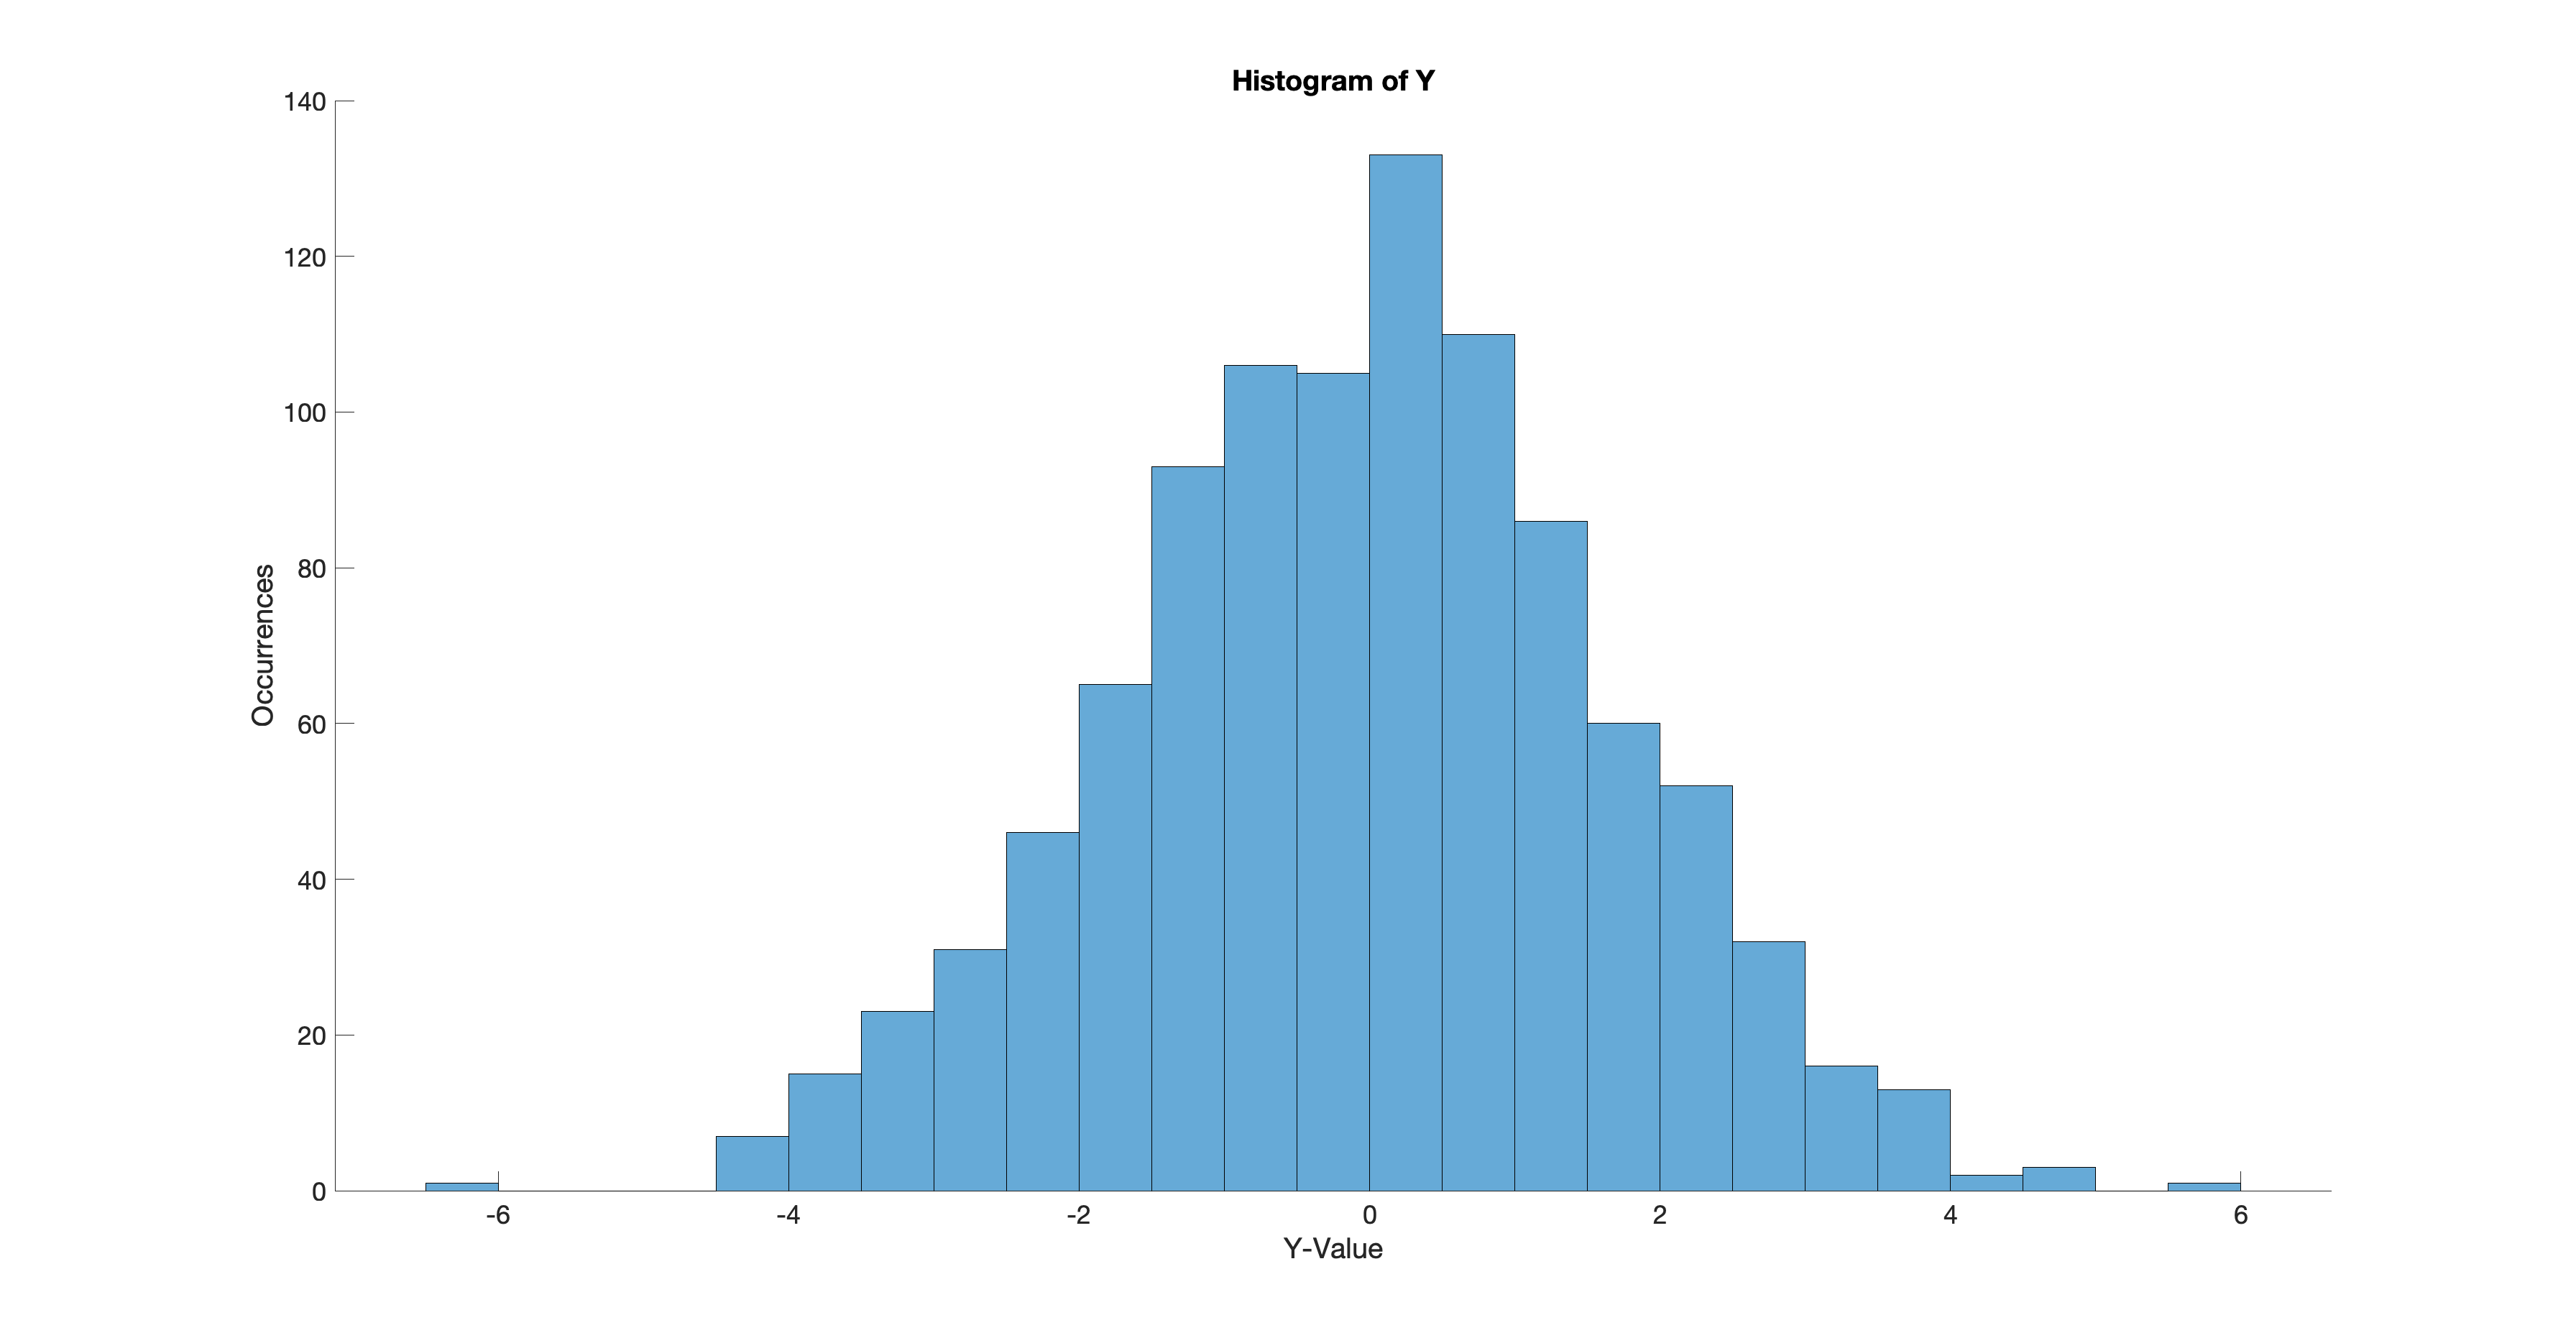
\includegraphics[width=0.75\linewidth]{../figures/p1_histogram.png}\label{fig:p1_hist}
    \caption{Histogram of the Monte Carlo Simulation}
\end{figure}
\section*{Problem II}
Perform a 1000 run Monte-Carlo simulation (of 10 minutes) to look at the error growth of a
random walk (integrated white noise). Use a white noise with 1-sigma value of 0.1 and 0.01
and compare the results. Plot the mean and standard deviation of the Monte-Carlo simulation
along with one run of the simulation (show that the random walk is zero mean with a
standard deviation is $\sigma_{\int w} = \sigma_w \Delta t\sqrt{k} = \sigma_w\sqrt{t \Delta t}$ (where k is the sample number).

\subsection*{Solution}
\begin{figure}[H]
    \centering
    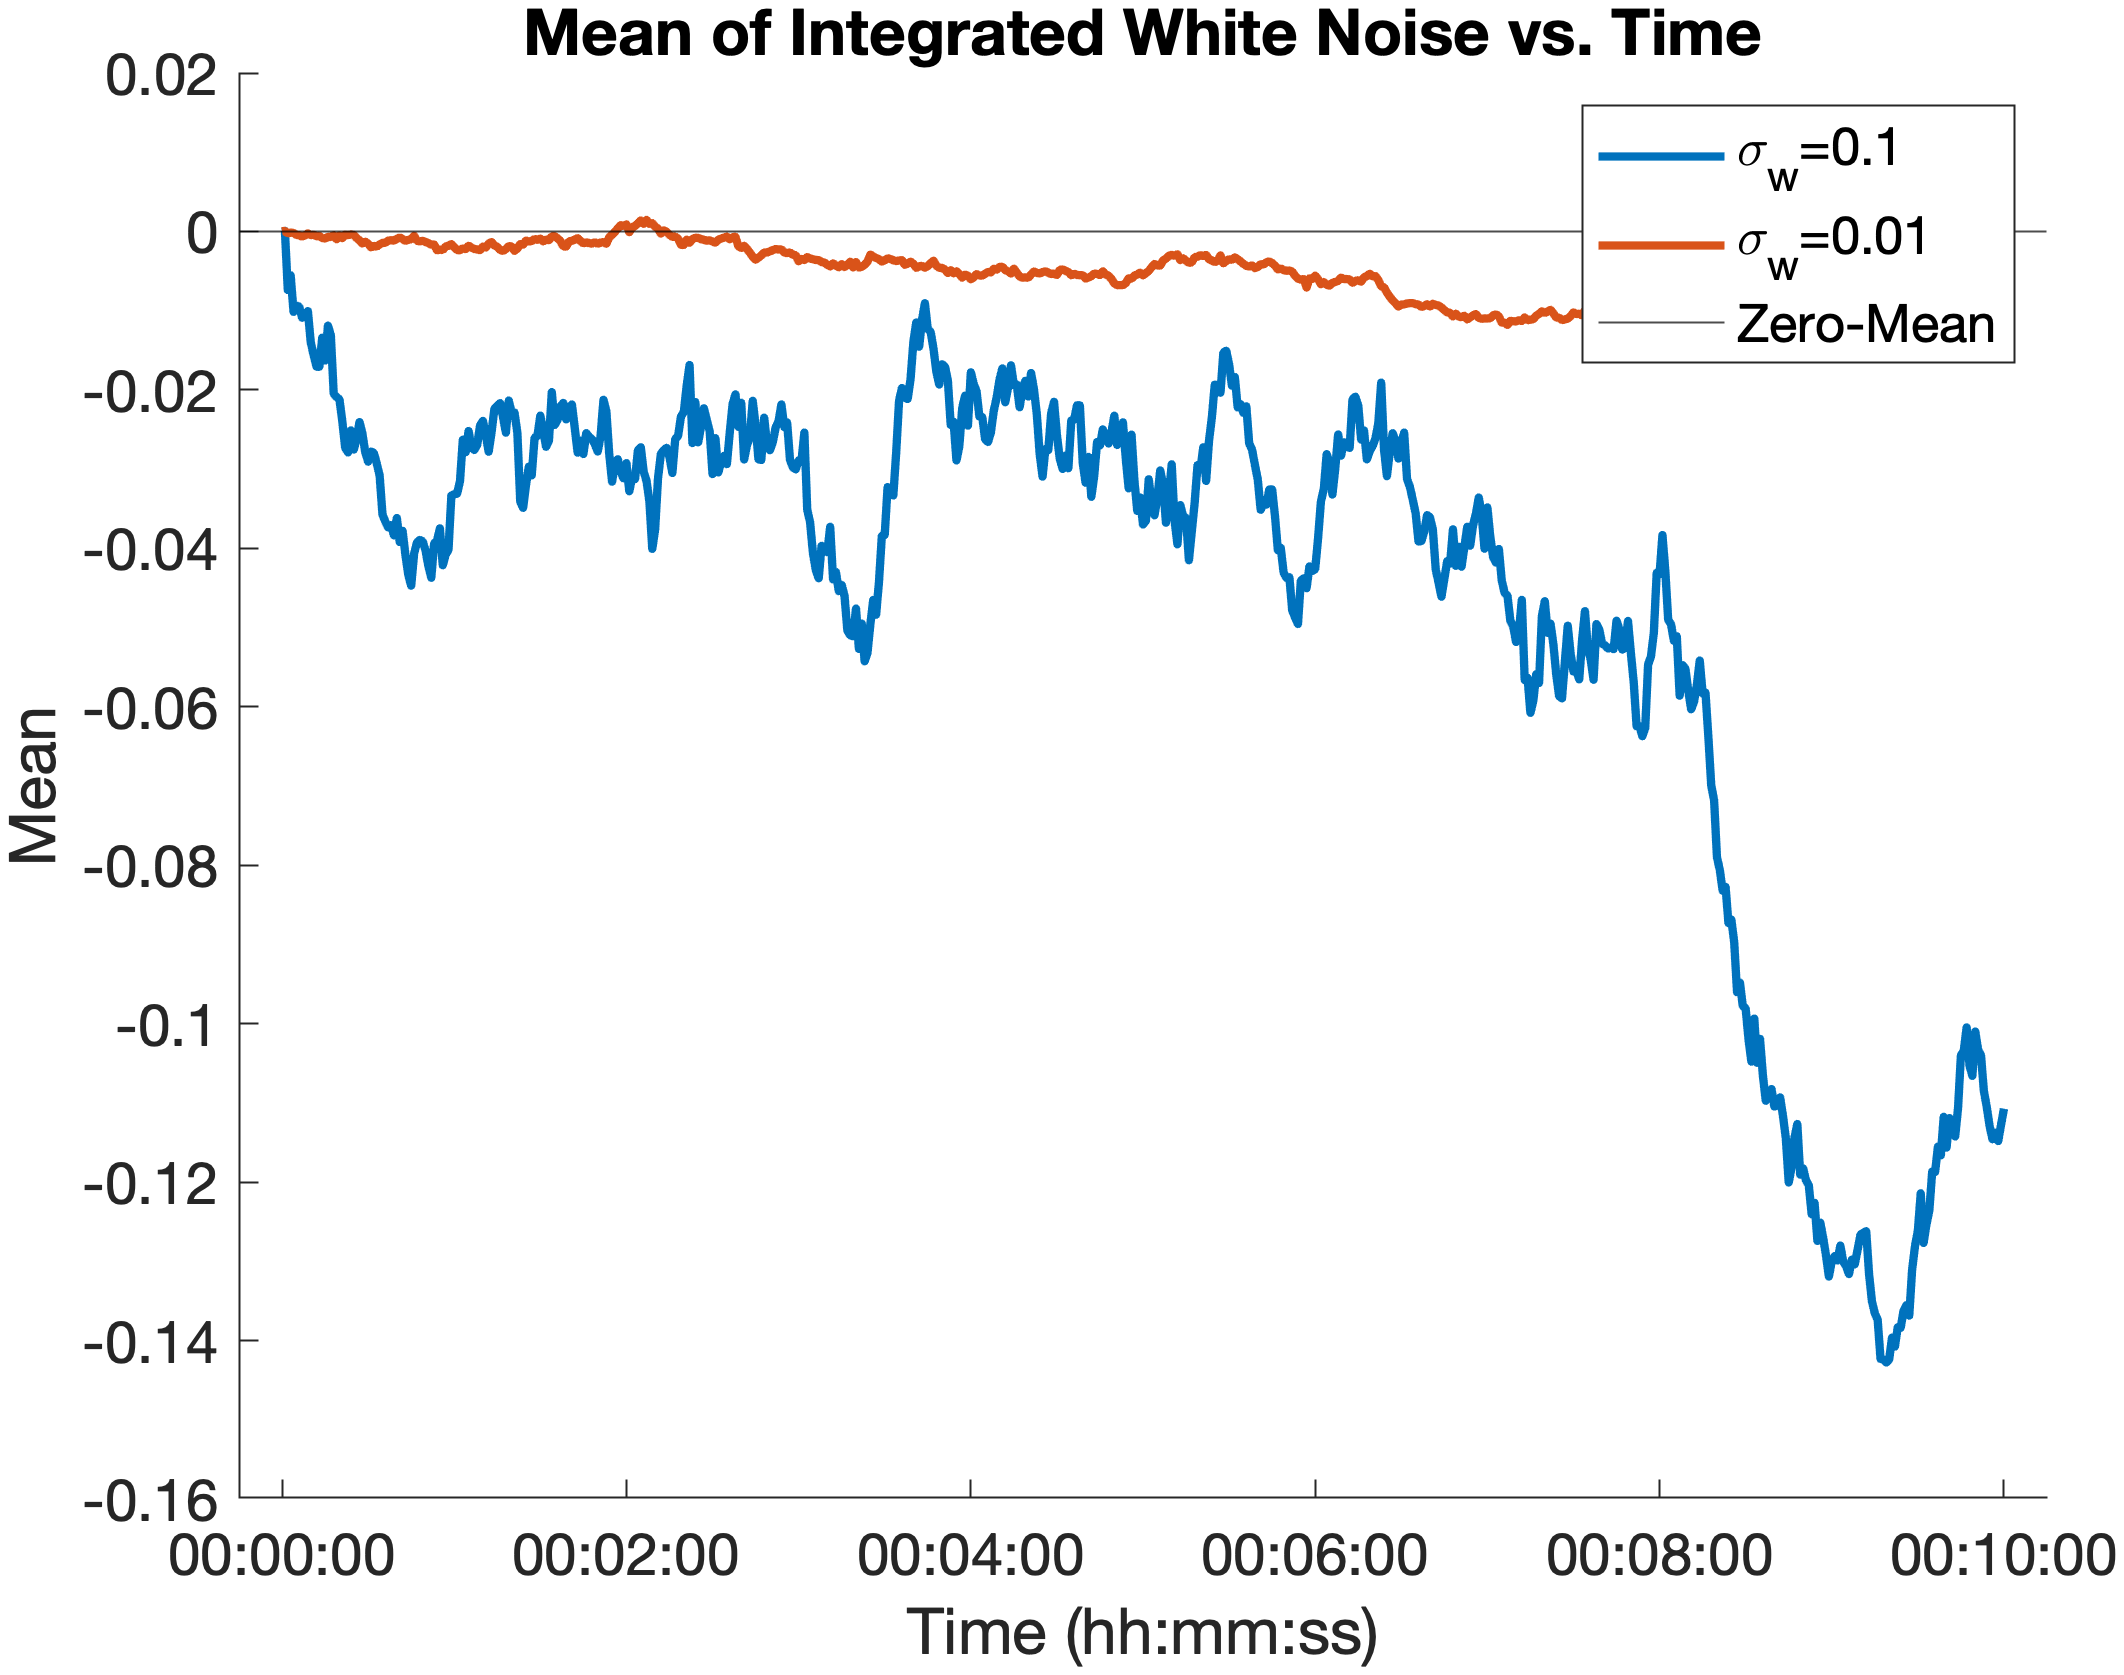
\includegraphics[width=0.75\linewidth]{../figures/p2_rw_mean.png}\label{fig:p2_rw_mean}
    \caption{Mean of the Monte Carlo Simulation of Random Walk}
\end{figure}

\begin{figure}[H]
    \centering
    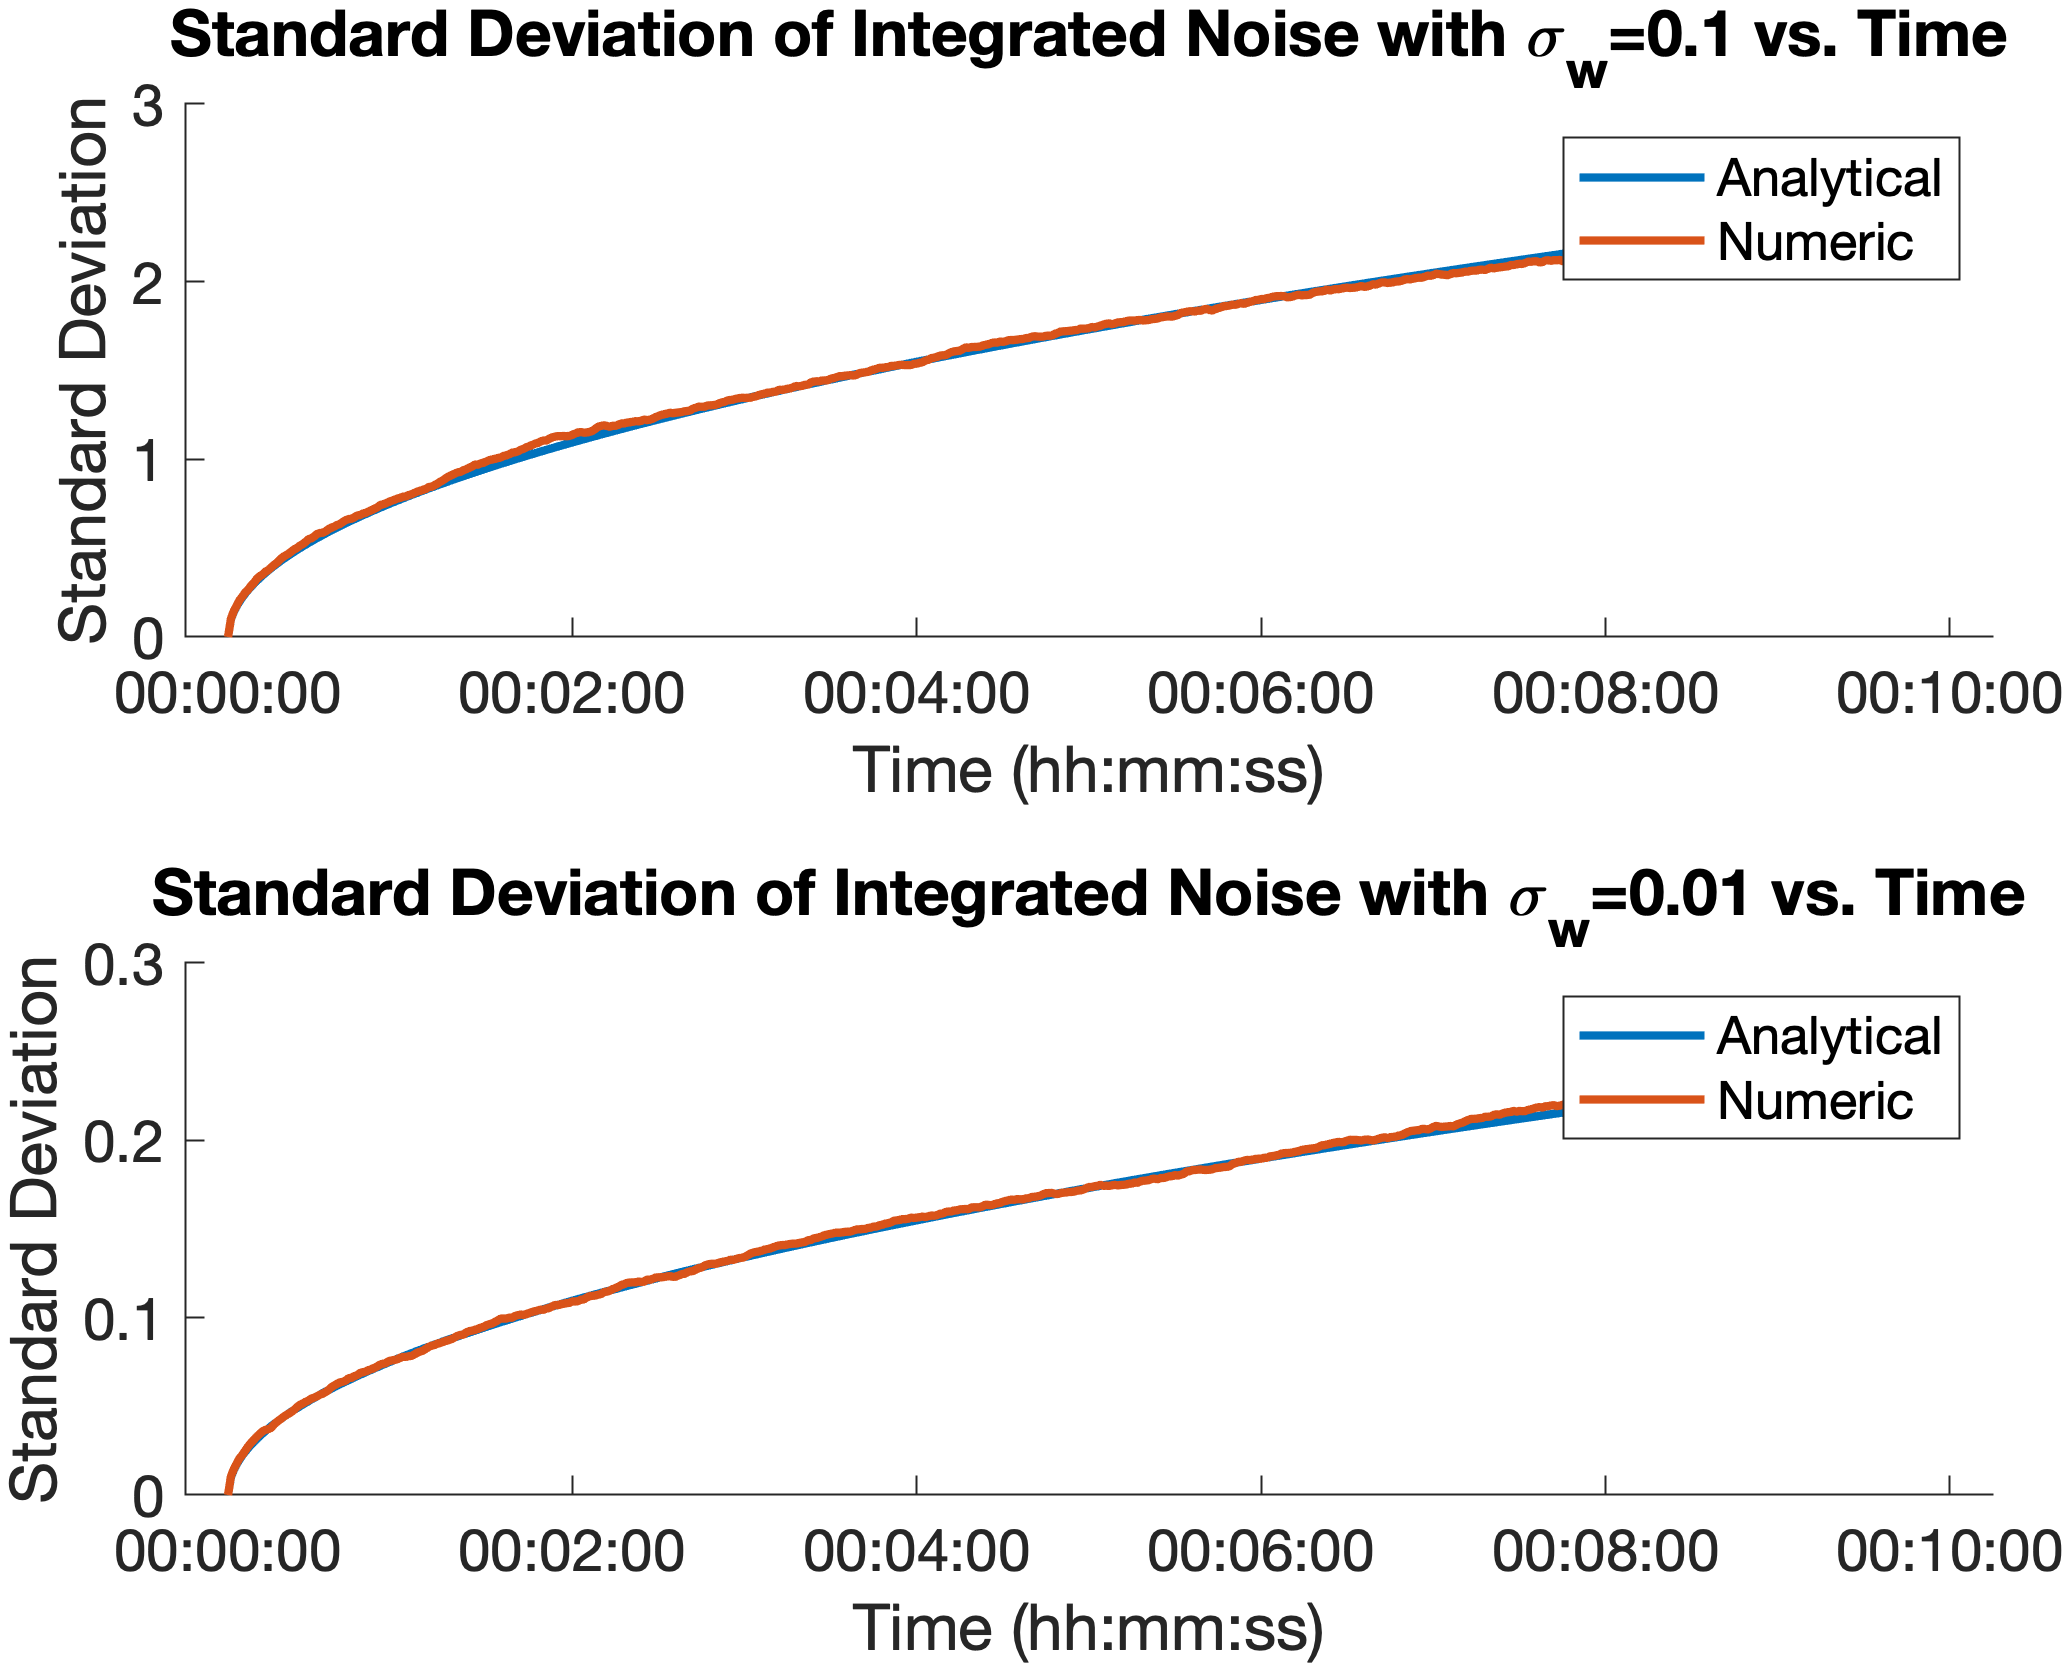
\includegraphics[width=0.75\linewidth]{../figures/p2_rw_sigma.png}\label{fig:p2_rw_sigma}
    \caption{Standard Deviation of the Monte Carlo Simulation of Random Walk}
\end{figure}

\subsection*{Bonus}
Provide a Histogram of the Monte-Carlo simulation at a few select time slots.

\subsection*{Solution}
\begin{figure}[H]
    \centering
    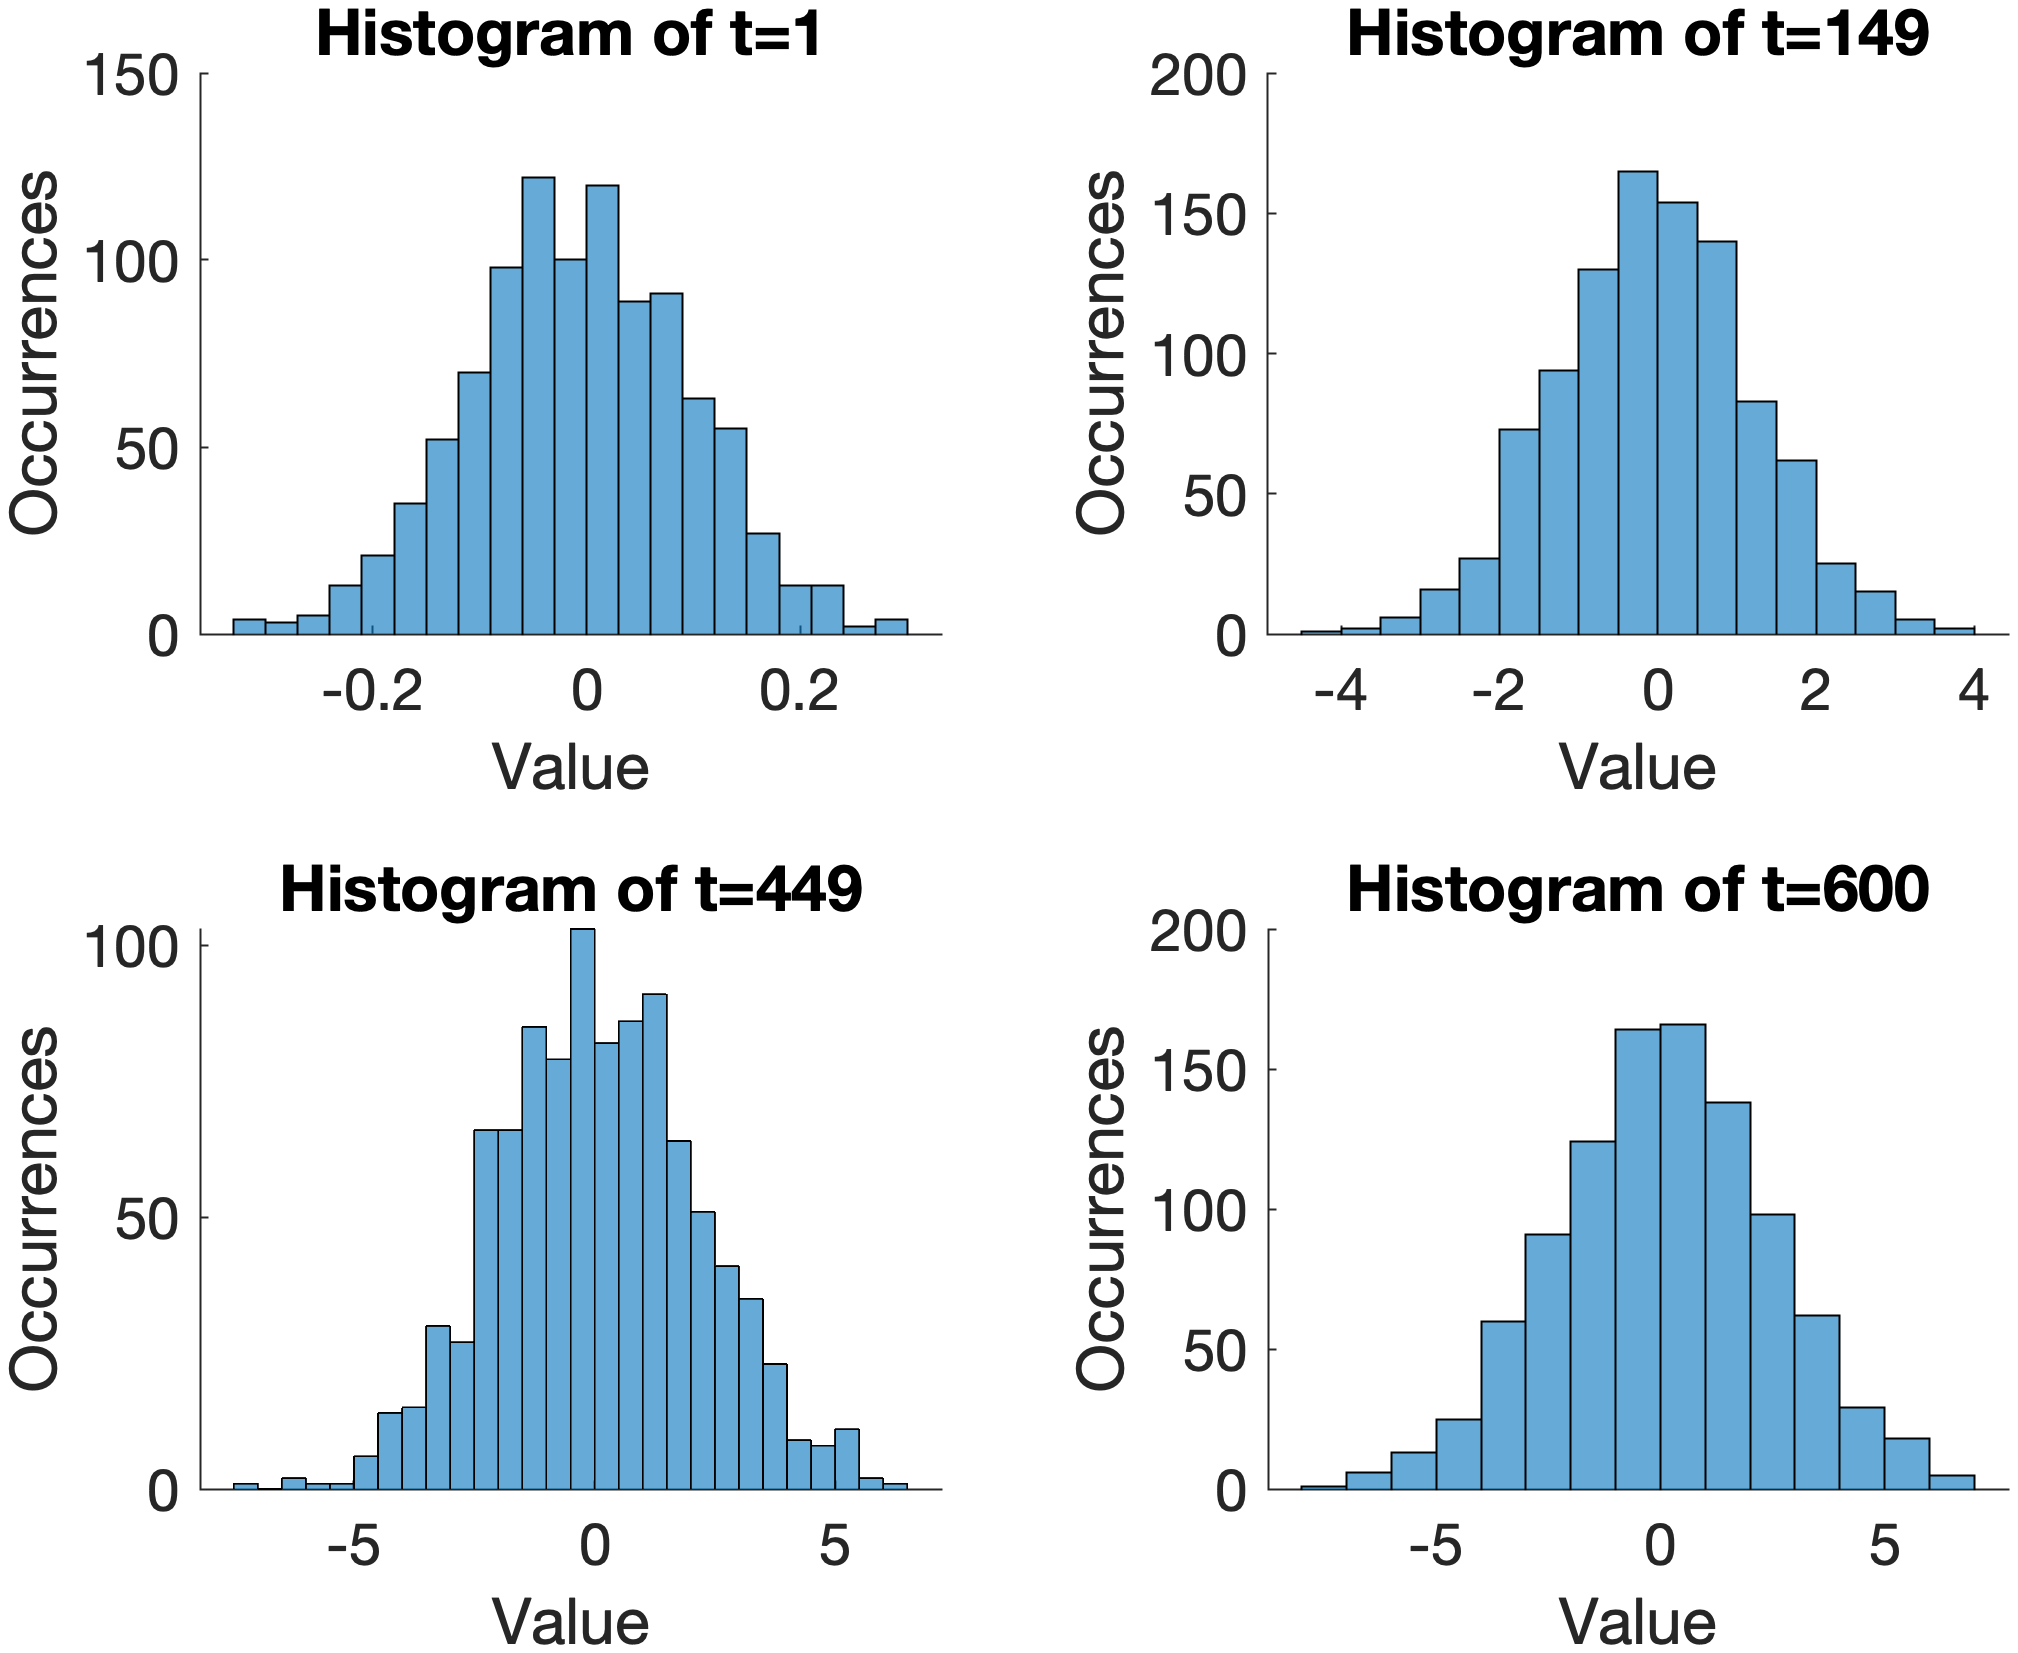
\includegraphics[width=0.75\linewidth]{../figures/p2_bonus.png}\label{fig:p2_bonus}
    \caption{Histograms of Individual Time Points}
\end{figure}

\subsection*{Part B}
Perform a 1000 Monte-Carlo simulation to look at the error growth of a 1st order Markov
process (integrated filtered noise) of the form $\dot{x} = -\frac{1}{\tau}x+w$. Use the same noise characteristics as above and compare the results with a 1 second and 100 second time
constant (this results in 4 combinations). Comment on how changing the time constant
and changing the standard deviation of the noise effects the error. Show that the 1st order
Markov process is zero mean with a standard deviation of is $\sigma_x = \sigma_w\Delta t\sqrt{\frac{A^{2t}-1}{A^2-1}}$ where $A = (1-\frac{\Delta t}{\tau})$. Note that for a positive time constant (i.e. stable system) the standard deviation has a steady-state value.

\subsection*{Solution}
\begin{figure}[H]
    \centering
    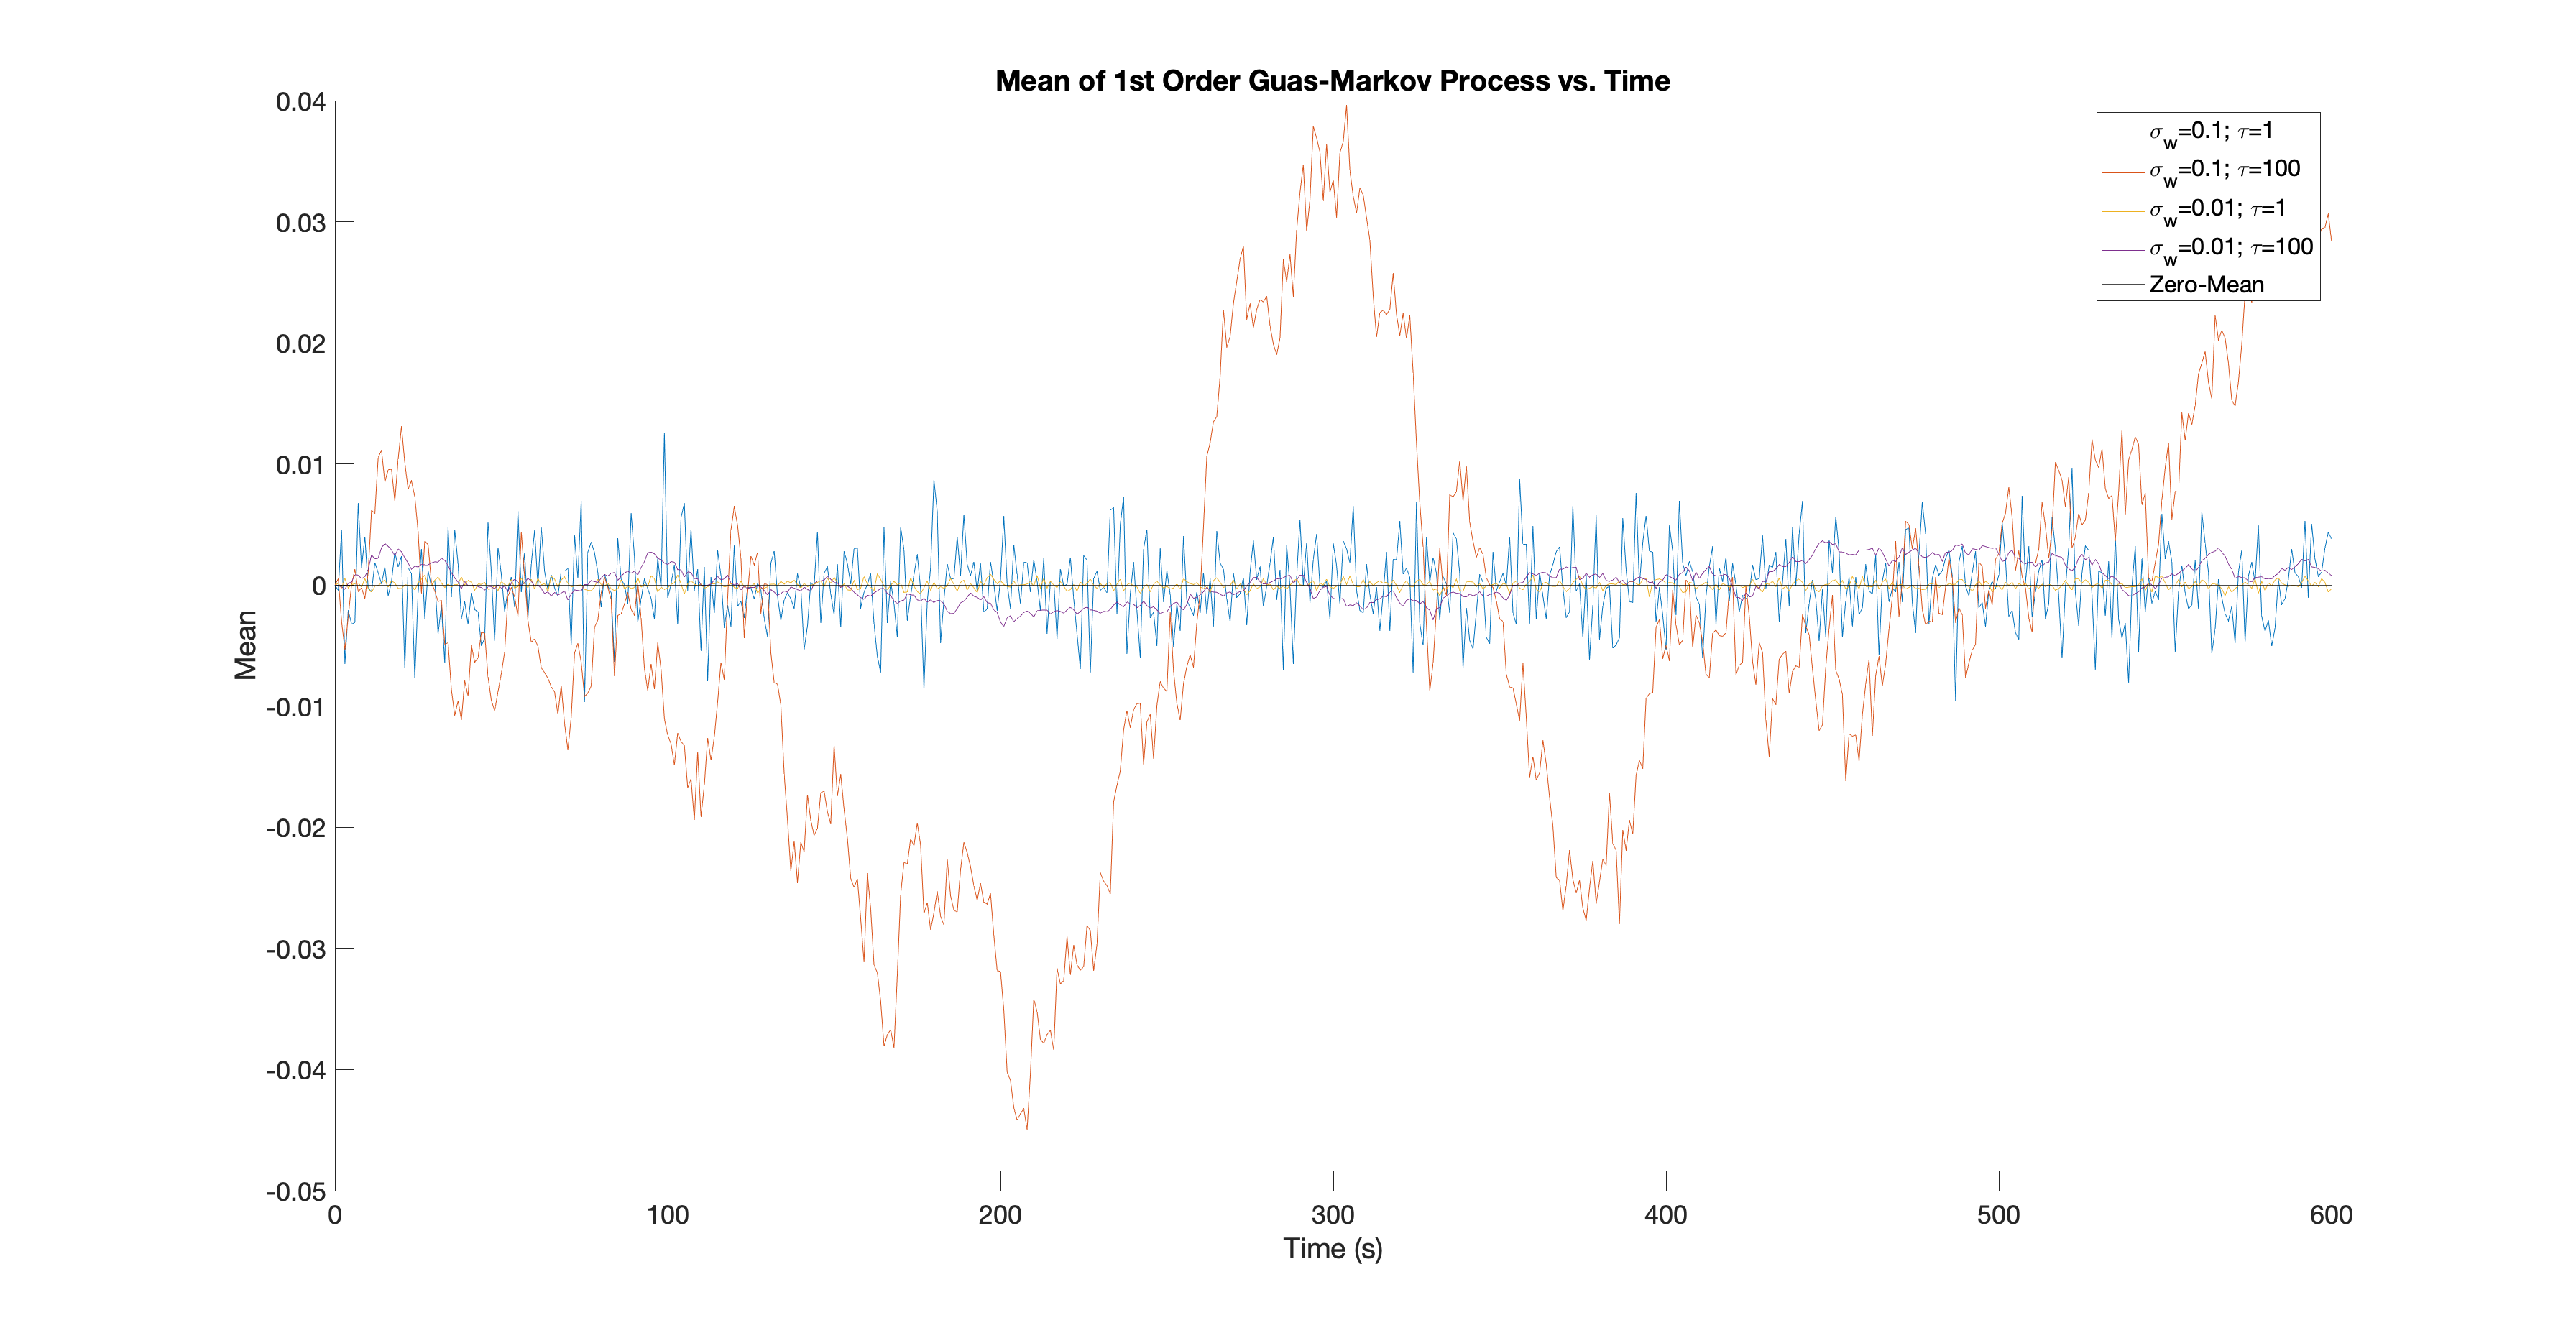
\includegraphics[width=0.75\linewidth]{../figures/p2_gm_mean.png}\label{fig:p2_gm_mean}
    \caption{Mean of the Monte Carlo Simulation of Gauss Markov}
\end{figure}

\begin{figure}[H]
    \centering
    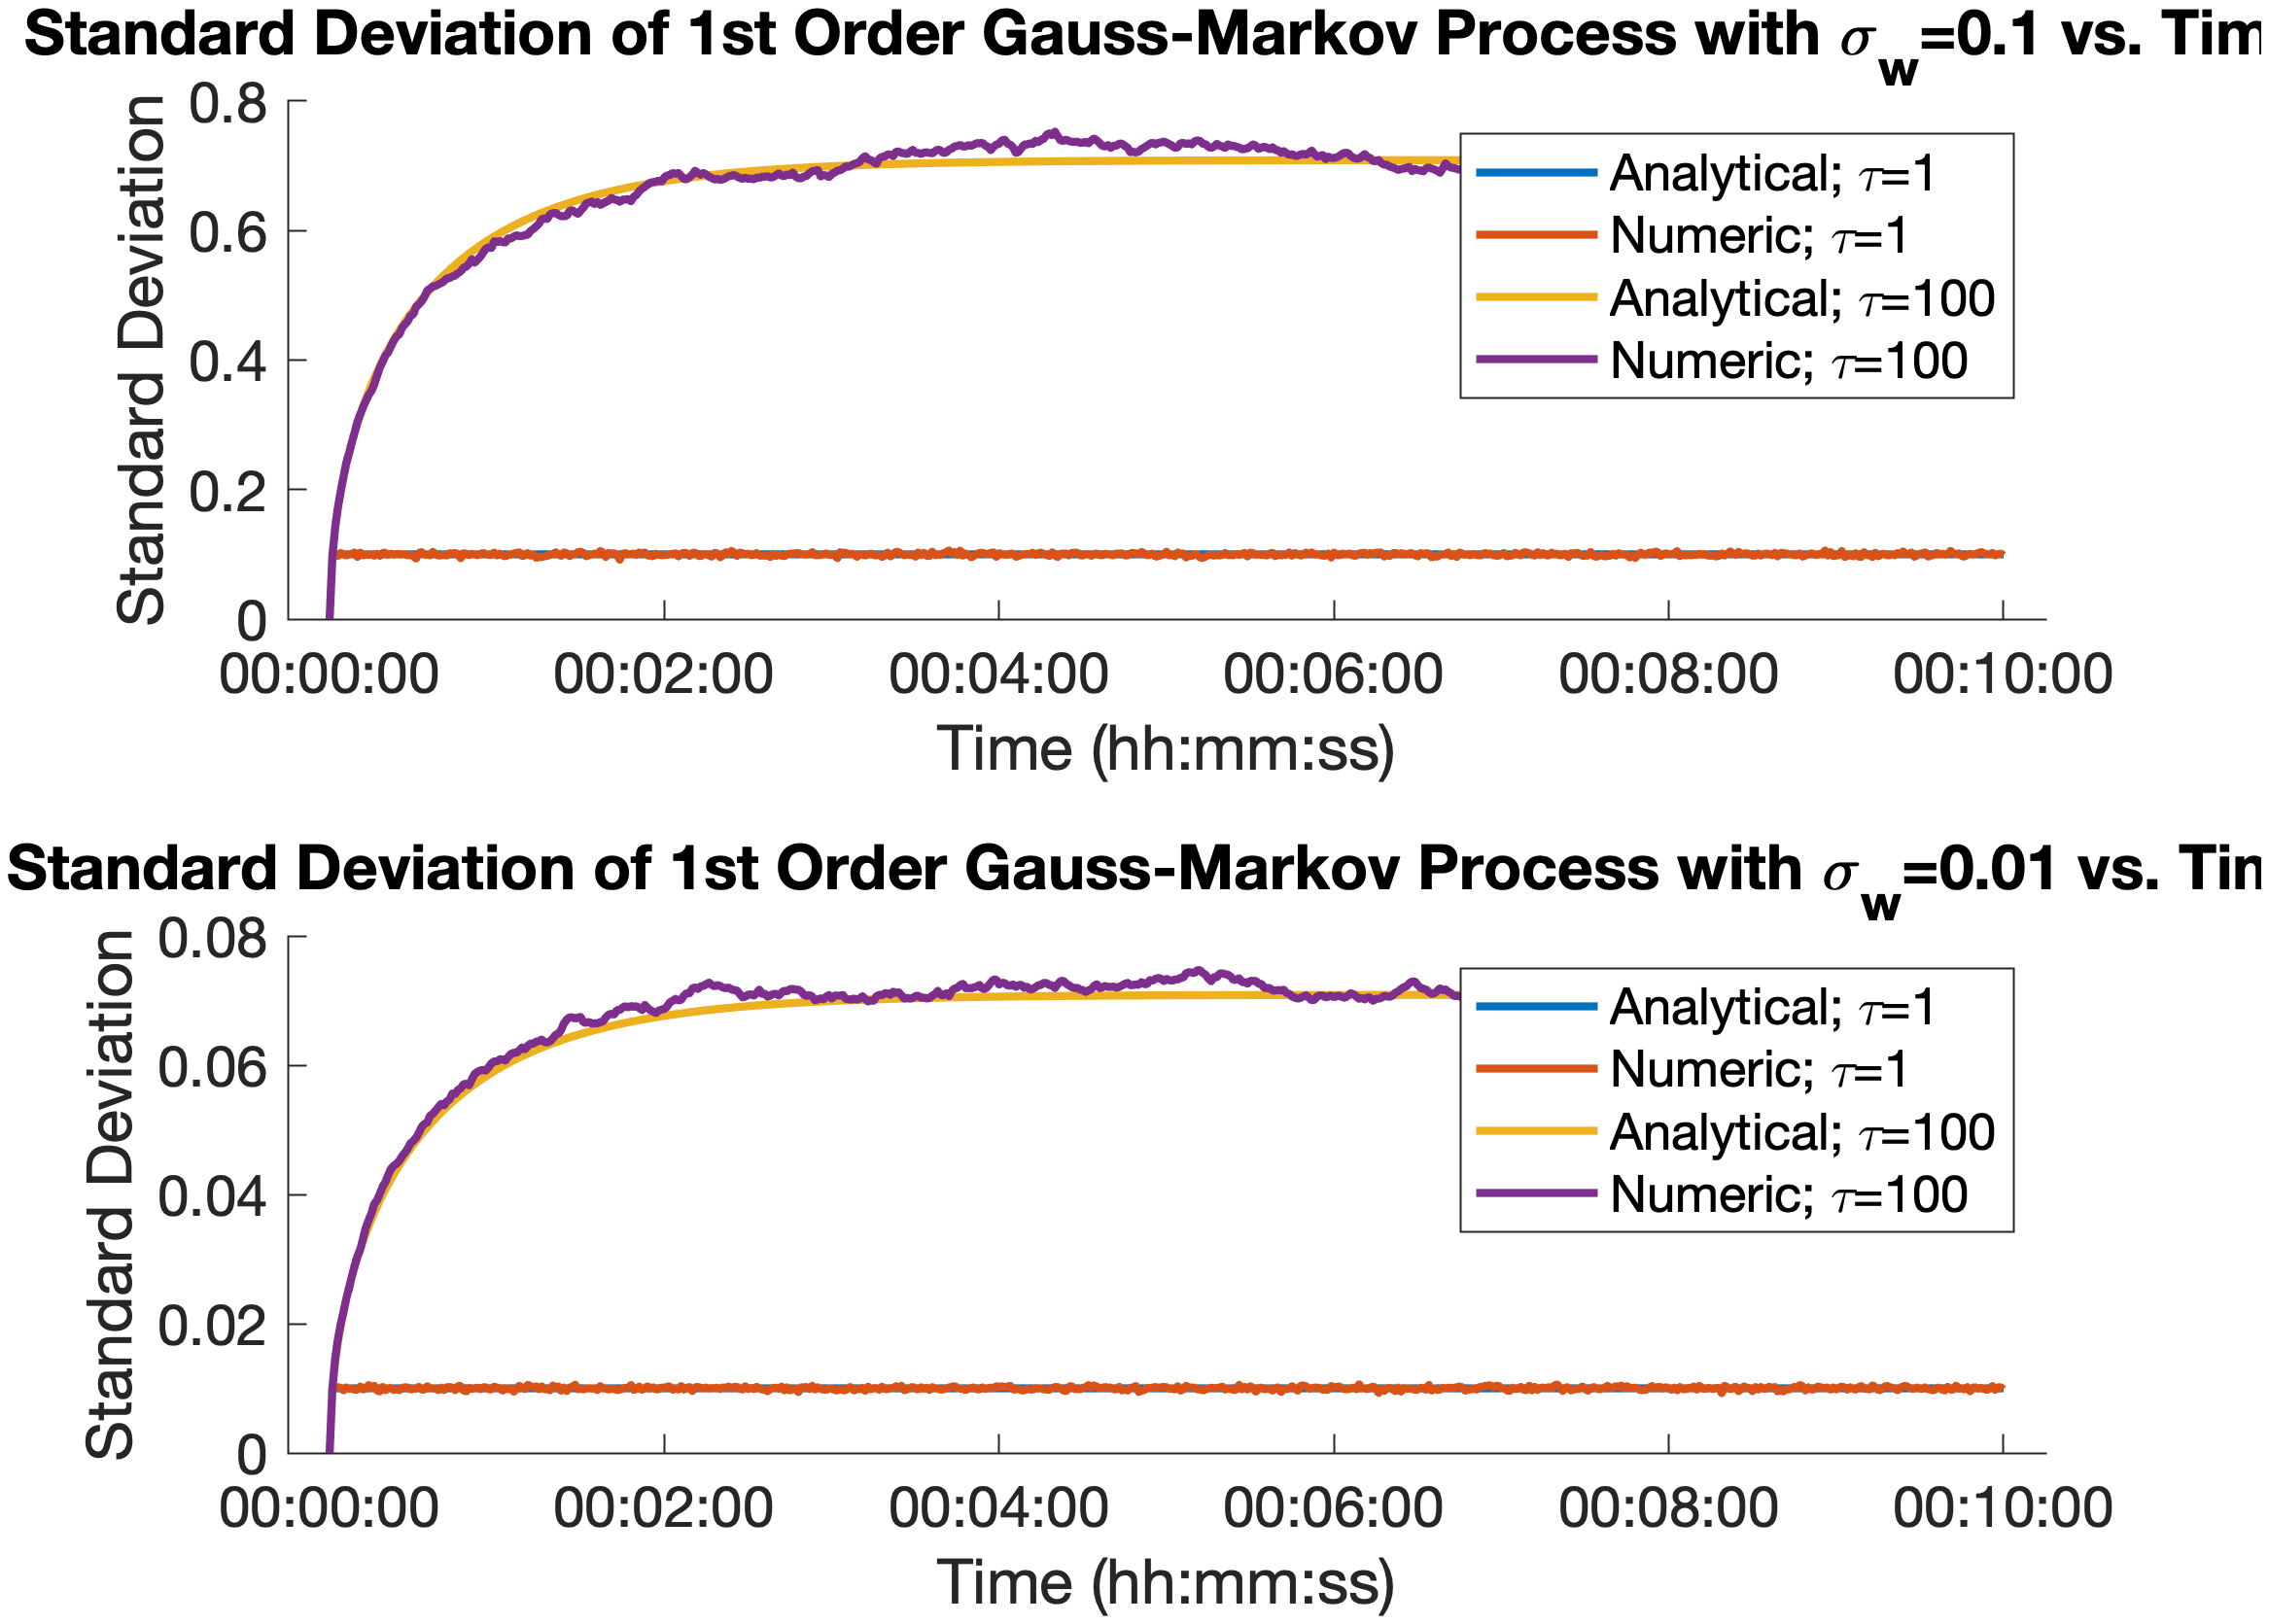
\includegraphics[width=0.75\linewidth]{../figures/p2_gm_sigma.png}\label{fig:p2_gm_sigma}
    \caption{Standard Deviation of the Monte Carlo Simulation of Gauss Markov}
\end{figure}

\section*{Problem III}
Determine the expected uncertainty for an L1-L5 ionosphere free pseudorange measurement
and L2-L5 ionosphere free pseudorange. Assuming all measurements have the same
accuracy (L1, L2, L5) which will provide the best ionosphere estimate?
\subsection*{Solution}
The equation for a pseudorange can be found in \Cref{eq:pseudorange}

\begin{equation}
    \rho = r + c\delta t + I + M + T + \nu_{rcvr}\label{eq:pseudorange}
\end{equation}

The only non-deterministic part of \Cref{eq:pseudorange} is the receiver noise, $\nu_{rcvr}$.  The equation for an L1+L2 Ionospheric-Free pseudorange is shown in \Cref{eq:IF_pseudorange}

\begin{equation}
    \rho_{IF} = \frac{f_{L1}^2}{f_{L1}^2 - f_{L2}^2}\rho_{L1} + \frac{f_{L2}^2}{f_{L1}^2 - f_{L2}^2}\rho_{L2}\label{eq:IF_pseudorange}
\end{equation}

If we subtract off the pseudorange itself, and consider the fact that the receiver noise is the only non-determinant part of the pseudorange equation, we can turn \Cref{eq:IF_pseudorange} into the following:

\begin{equation}
    \delta \rho_{IF} = \frac{f_{L1}^2}{f_{L1}^2 - f_{L2}^2}\nu_{rcvr} + \frac{f_{L2}^2}{f_{L1}^2 - f_{L2}^2}\nu_{rcvr}\label{eq:IF_del_psr}
\end{equation}

The receiver noises are not frequency-dependent, so given the signals are read with the same receiver, the noises would be equal.  Following \Cref{eq:IF_del_psr} through algebraically, the $\sigma$ on $\delta \rho$ is:

\begin{gather*}
    E \left[(\delta\rho_{IF})^2\right] = E \left[(\frac{f_{L1}^2}{f_{L1}^2 - f_{L2}^2}\nu_{rcvr} + \frac{f_{L2}^2}{f_{L1}^2 - f_{L2}^2}\nu_{rcvr})\right]\\
    E \left[(\delta\rho_{IF})^2\right] = \frac{f_{L1}^2}{f_{L1}^2 - f_{L2}^2}E \left[\nu_{rcvr}\right] + \frac{f_{L2}^2}{f_{L1}^2 - f_{L2}^2}E \left[\nu_{rcvr}\right]\\
    \sigma_{\rho_{IF}}^2 =  \frac{f_{L1}^2}{f_{L1}^2 - f_{L2}^2}\sigma_{rcvr}^2 + \frac{f_{L2}^2}{f_{L1}^2 - f_{L2}^2}\sigma_{rcvr}^2\\
    \sigma_{\rho_{IF}}^2 =  \sigma_{rcvr}^2(\frac{f_{L1}^2}{f_{L1}^2 - f_{L2}^2} + \frac{f_{L2}^2}{f_{L1}^2 - f_{L2}^2})\\
    \sigma_{\rho_{IF}} =  \sqrt{\sigma_{rcvr}^2(\frac{f_{L1}^2}{f_{L1}^2 - f_{L2}^2} + \frac{f_{L2}^2}{f_{L1}^2 - f_{L2}^2})}\\
\end{gather*}

Using the above equation for the standard deviation on the Ionospheric-Free pseudorange, an estimate of that value can be calculated for any combination of frequencies, just replacing $f_{L1}$ and $f_{L2}$ with the utilized frequencies.  Doing this shows that L1+L5 is the best combination for obtaining Ionospheric-Free psuedoranges as it produces the smallest standard deviation.

\section*{Problem IV}
Show that the differential GPS problem is linear. In other words derive the following
expression:
    \begin{center}
    $\Delta\rho=\begin{bmatrix}
        uv_x & uv_y & uv_z & 1
        \end{bmatrix}\begin{bmatrix}
        r_x\\r_y\\r_z\\c\delta t_{ab}
        \end{bmatrix}$
    \end{center}
\subsection*{Solution}

To show the problem of differential GPS is linear, it begins with the nonlinear, matrix equation for the user's pseudorange as shown in \Cref{eq:psr_mat}

\begin{equation}
    \rho_u = \begin{bmatrix}
        uv_x & uv_y & uv_z & 1
        \end{bmatrix}\begin{bmatrix}
        \delta x_u\\\delta y_u\\\delta z_u\\c\delta t_u
        \end{bmatrix}\label{eq:psr_mat}
\end{equation}

Taking \Cref{eq:psr_mat} and differencing it with a similar equation for the base station, the following equation comes out:

\begin{equation}
    \Delta\rho = \begin{bmatrix}
        uv_x & uv_y & uv_z & 1
        \end{bmatrix}\begin{bmatrix}
        \delta x_u - \delta x_b\\\delta y_u - \delta y_b\\\delta z_u - \delta z_b\\c\delta t_u - c\delta t_b
        \end{bmatrix}\label{eq:del_psr_mat}
\end{equation}

Given that $\delta x = x - \hat{x}$ and it is assumed that the base and user are close enough that $\hat{x_u}$ and $\hat{x_b}$ are the same, the above equation reduces to:

\begin{center}
$\Delta\rho=\begin{bmatrix}
    uv_x & uv_y & uv_z & 1
    \end{bmatrix}\begin{bmatrix}
    r_x\\r_y\\r_z\\c\delta t_{ab}
    \end{bmatrix}$
\end{center}


\section*{Problem V}
Set up your own 2D planar trilateration problem. Place the SVs at (0,300) (100,400),
(700,400), and (800,300). Generate a range measurement for a base station at (400,0) and a
user at (401,0).

\subsection*{Part A}
Solve for the position of the user using 2 SVs and then 4 SVs assuming no clock
errors. How does the PDOP change for the two cases?

\subsection*{Part B}
Solve for the position of the user assuming you need to solve for the user clock bias.
What is the PDOP with all 4 satellites.

\subsection*{Part C}
Calculate a differential solution between the base and user using a single difference
model and assuming you must solve for a clock bias between the base station and
user. What is the PDOP with all 4 satellites?

\subsection*{Part D}
Calculate a differential solution between the base and user using a double difference
model to remove the clock bias between the base station and user. What is the PDOP
with all 4 satellites?

\subsection*{Part E}
Assuming the range error is zero mean with unit variance, what is the order of
accuracy in the above 4 solution methods?

\subsection*{Solution}
\begin{figure}[H]
    \centering
    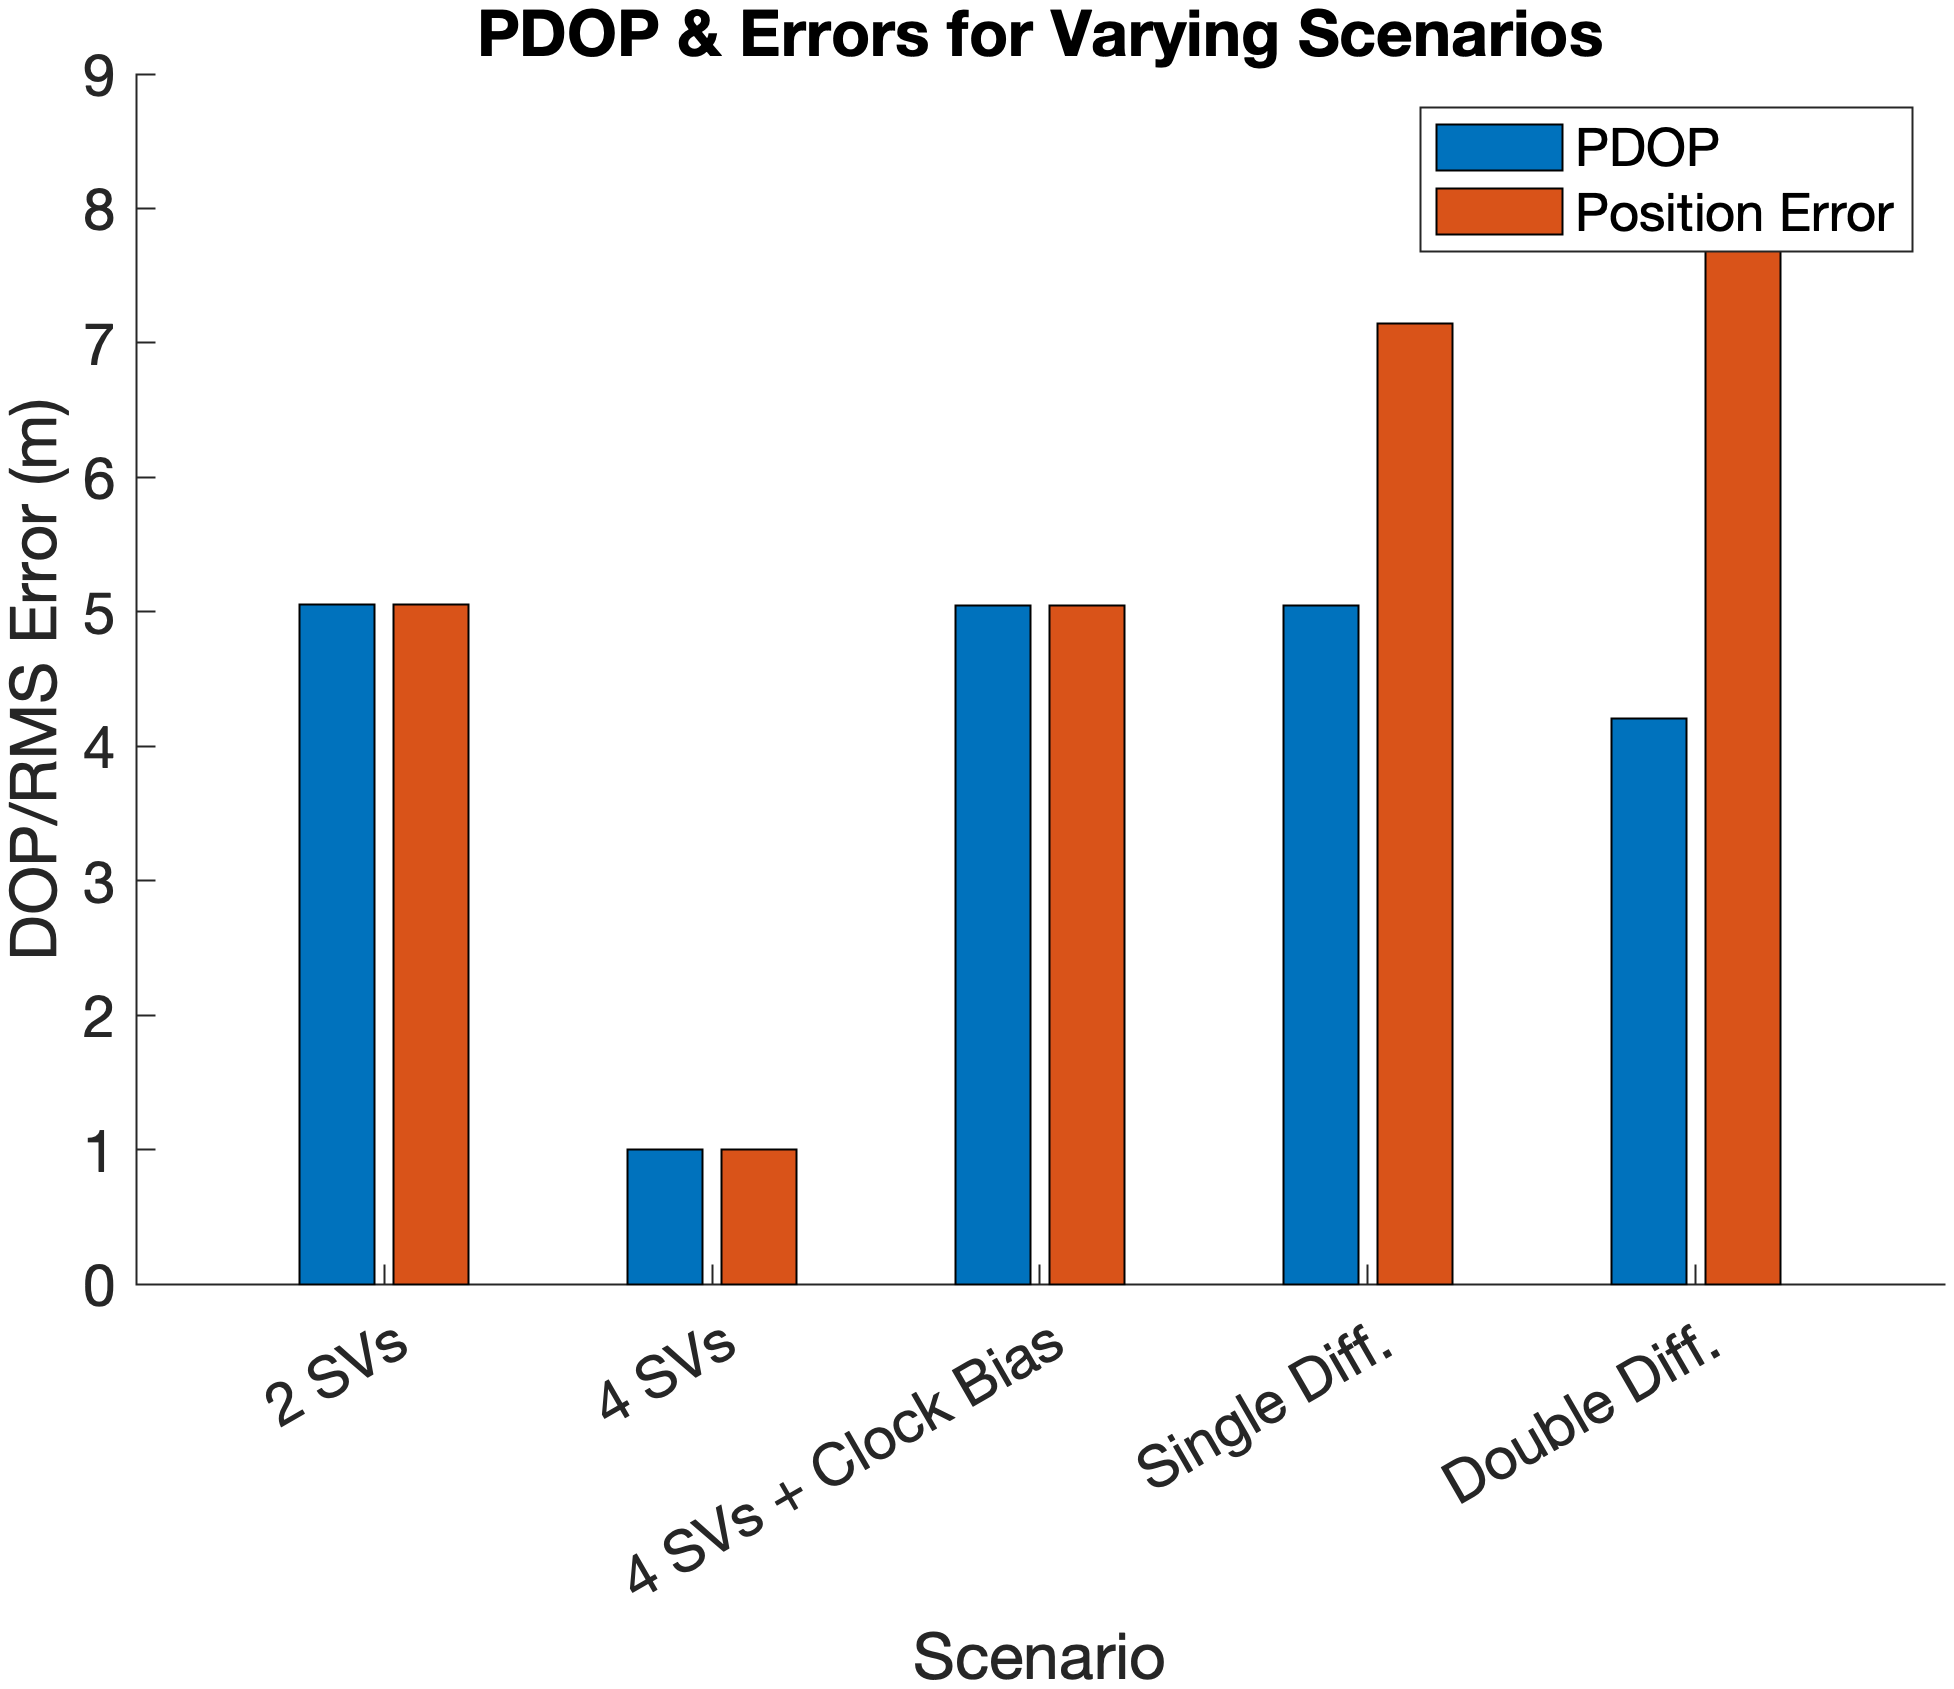
\includegraphics[width=0.75\linewidth]{../figures/p5_pdop.png}\label{fig:p5_pdop}
    \caption{PDOP \& Error for Varying Circumstances}
\end{figure}

\section*{Problem VI}
(Bonus for Undergrads/Required for Grads). Repeat problem \#4 using 4 and 8 SV positions
from Lab \#2 (4,7,8,9,16,21,27,30). Comment on any difference or similarities with the
planar problem in \#3.

\subsection*{Solution}
\begin{figure}[H]
    \centering
    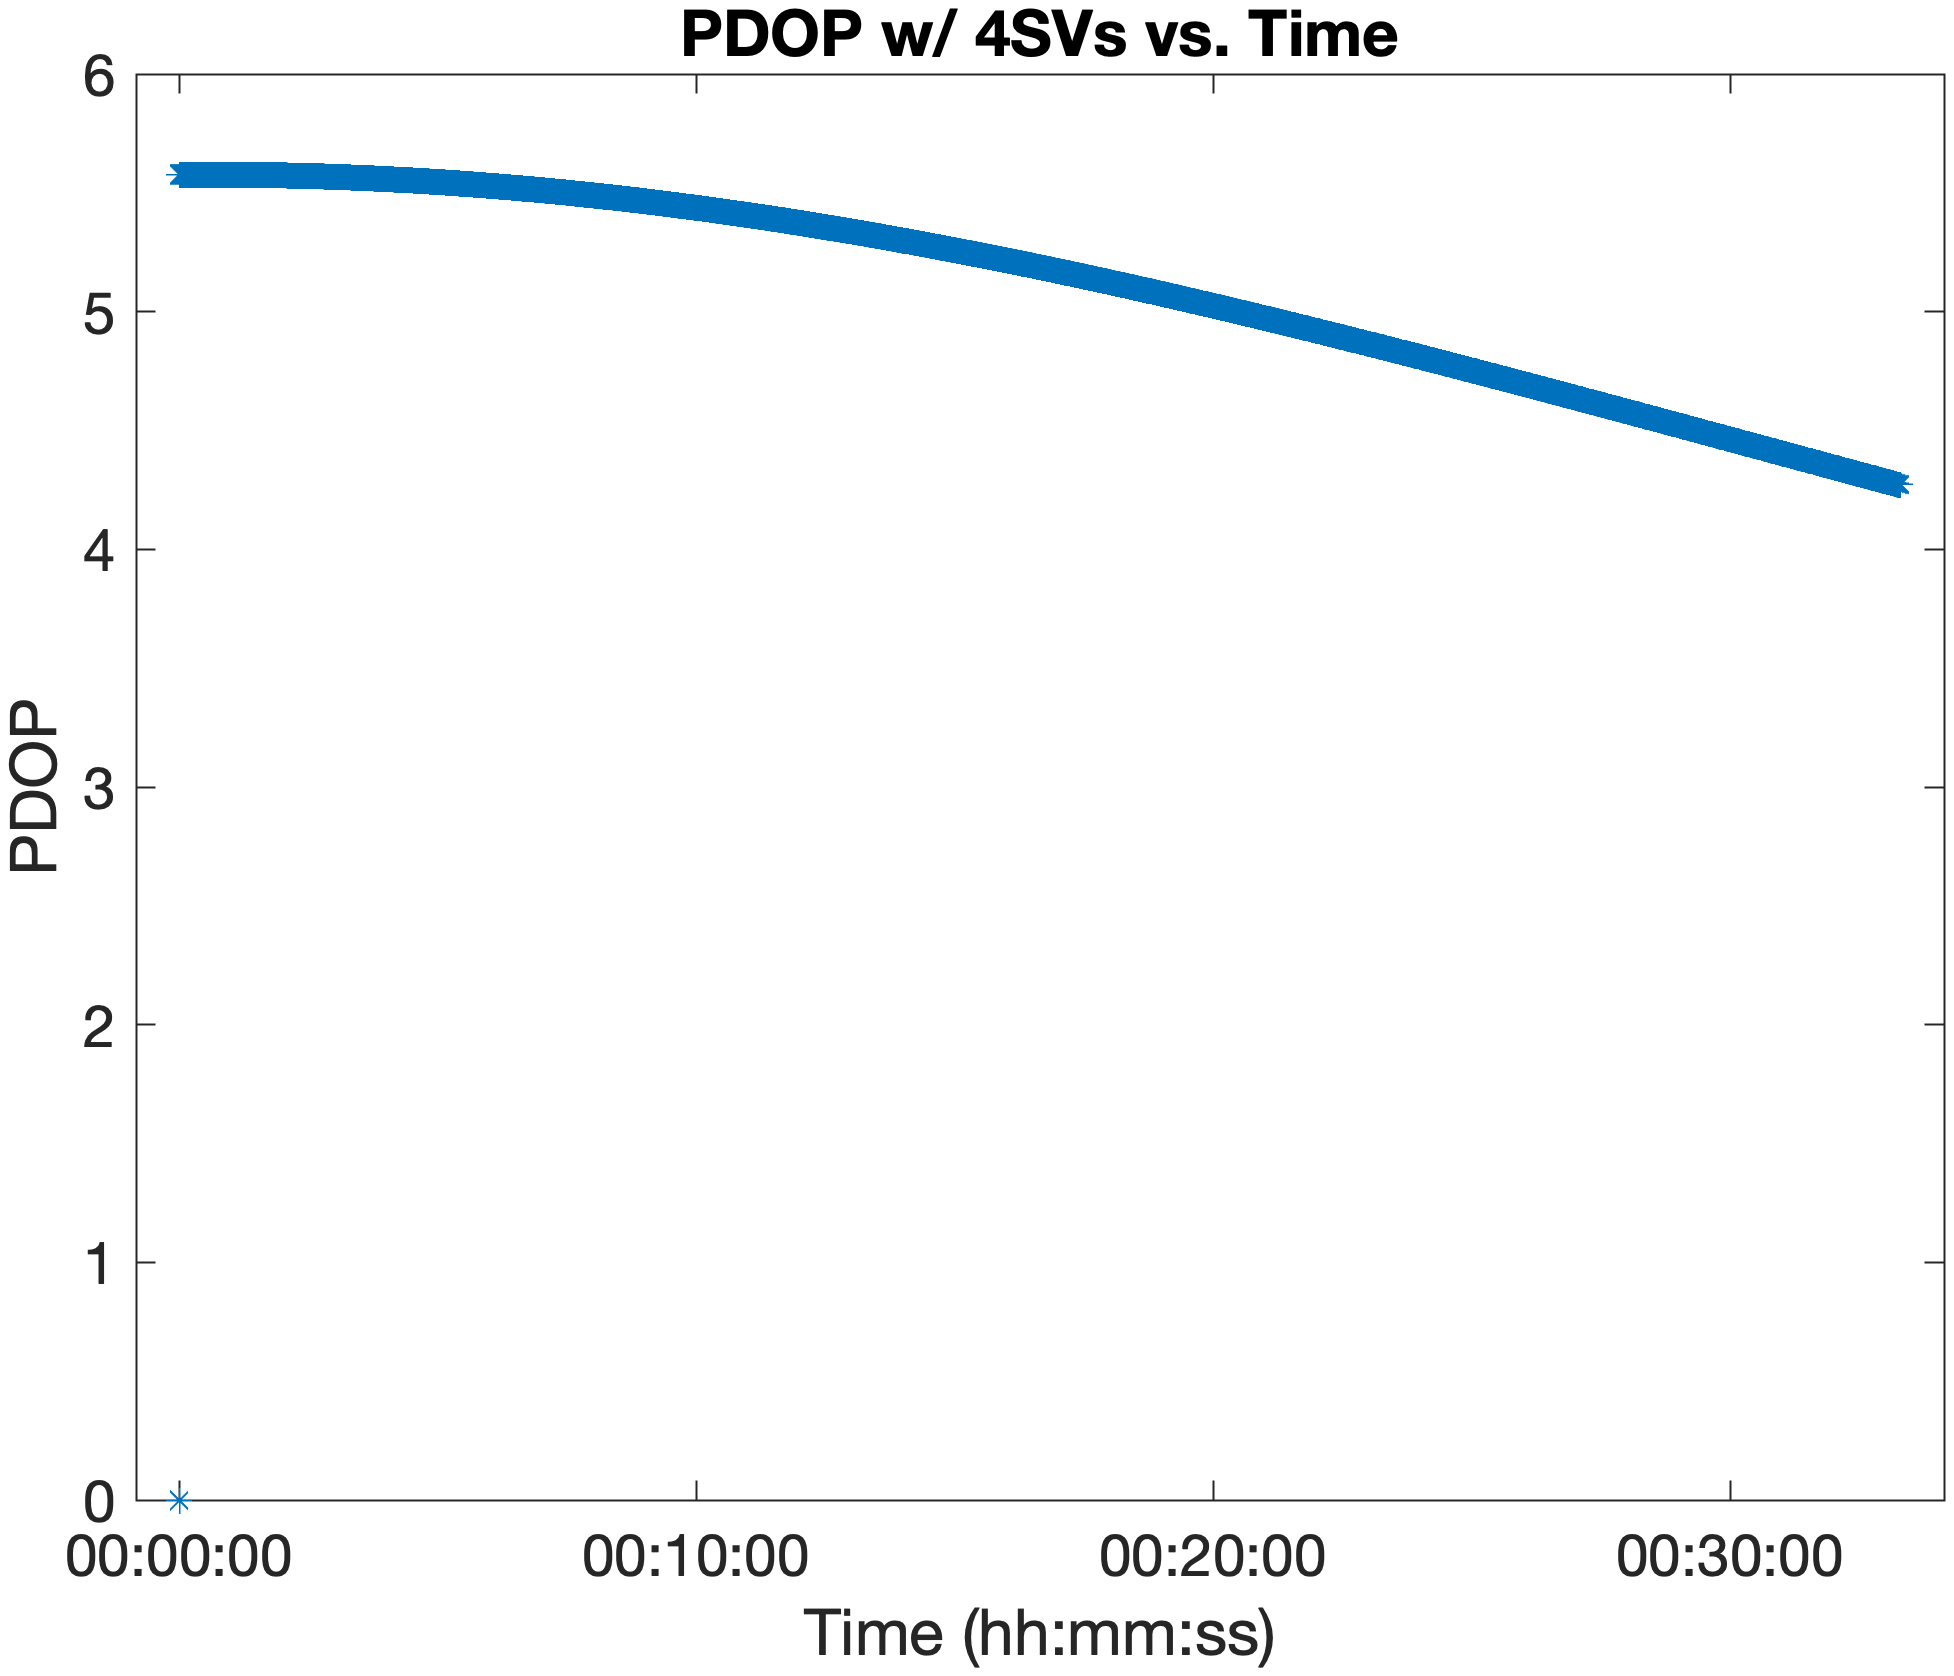
\includegraphics[width=0.75\linewidth]{../figures/p6_4svs_pdop.png}\label{fig:p6_4svs_pdop}
    \caption{PDOP for Real Data w/ 4SVs}
\end{figure}

\begin{figure}[H]
    \centering
    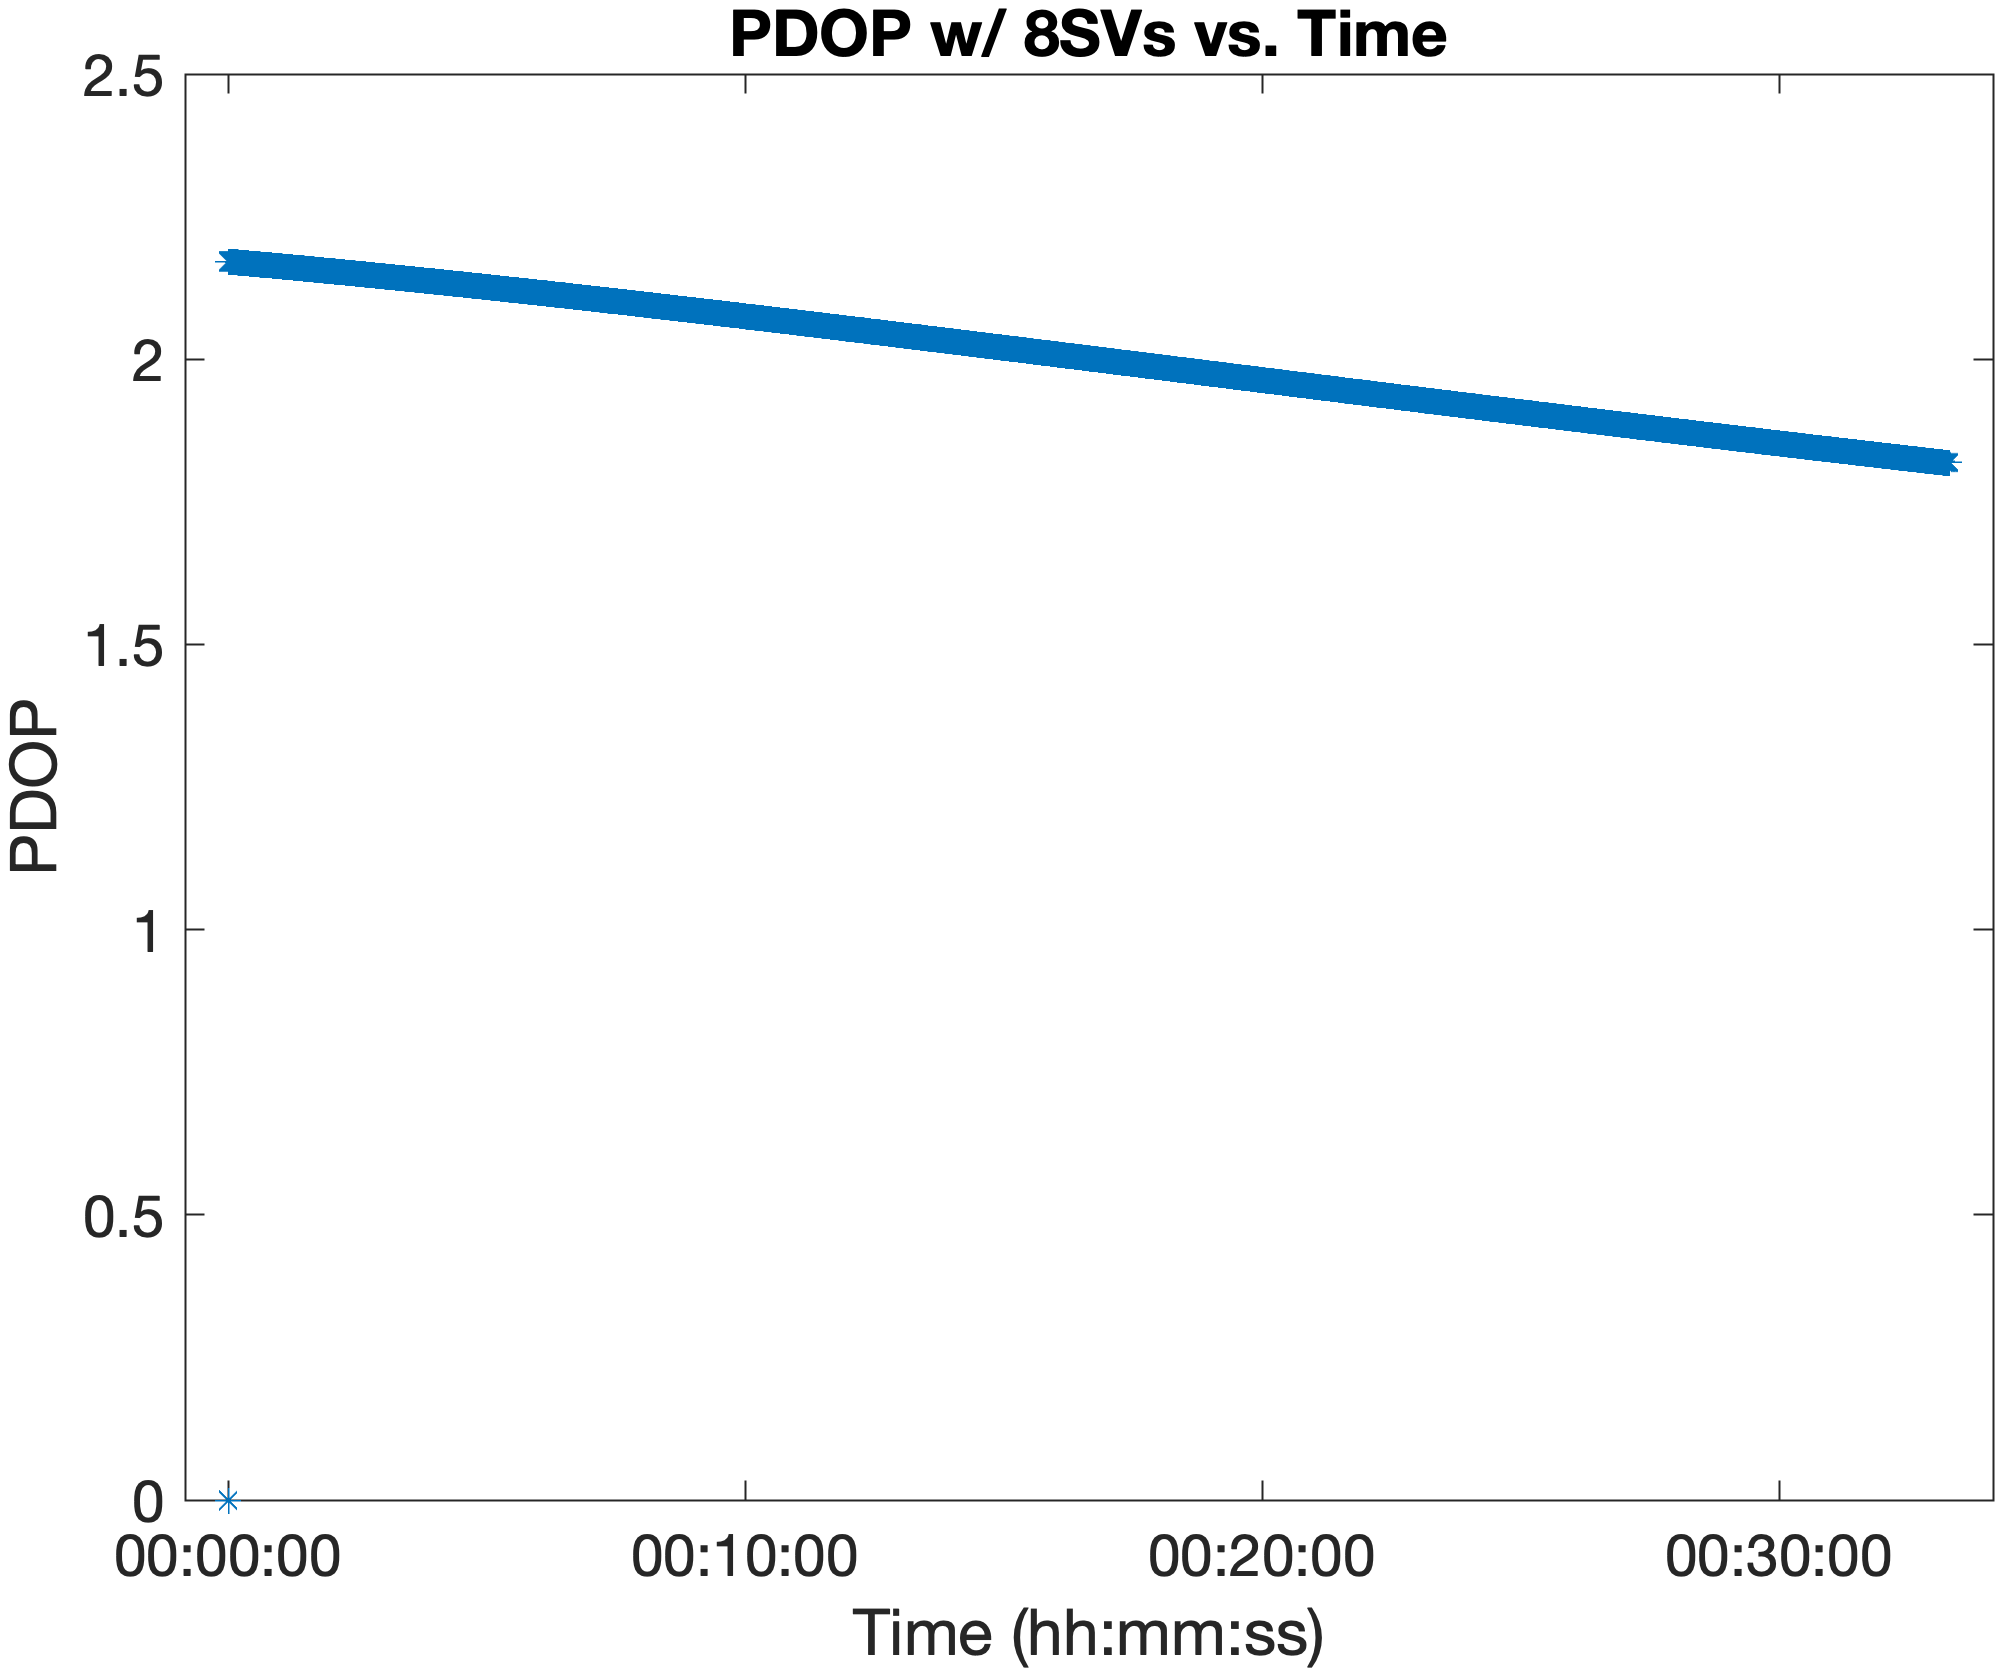
\includegraphics[width=0.75\linewidth]{../figures/p6_8svs_pdop.png}\label{fig:p6_8svs_pdop}
    \caption{PDOP for Real Data w/ 8SVs}
\end{figure}

Though not exact, the 4SV scenario with the real satellite data has a PDOP ~3x larger than the 8SV scenario.  This is around the same difference between the 4SV and 2SV scenarios in Part V.

\section*{Problem VII}
Chapter 2, Problem 1a and 1b for PRN \#4. Repeat 1a for PRN \#7

\subsection*{Solution}
\begin{figure}[H]
    \centering
    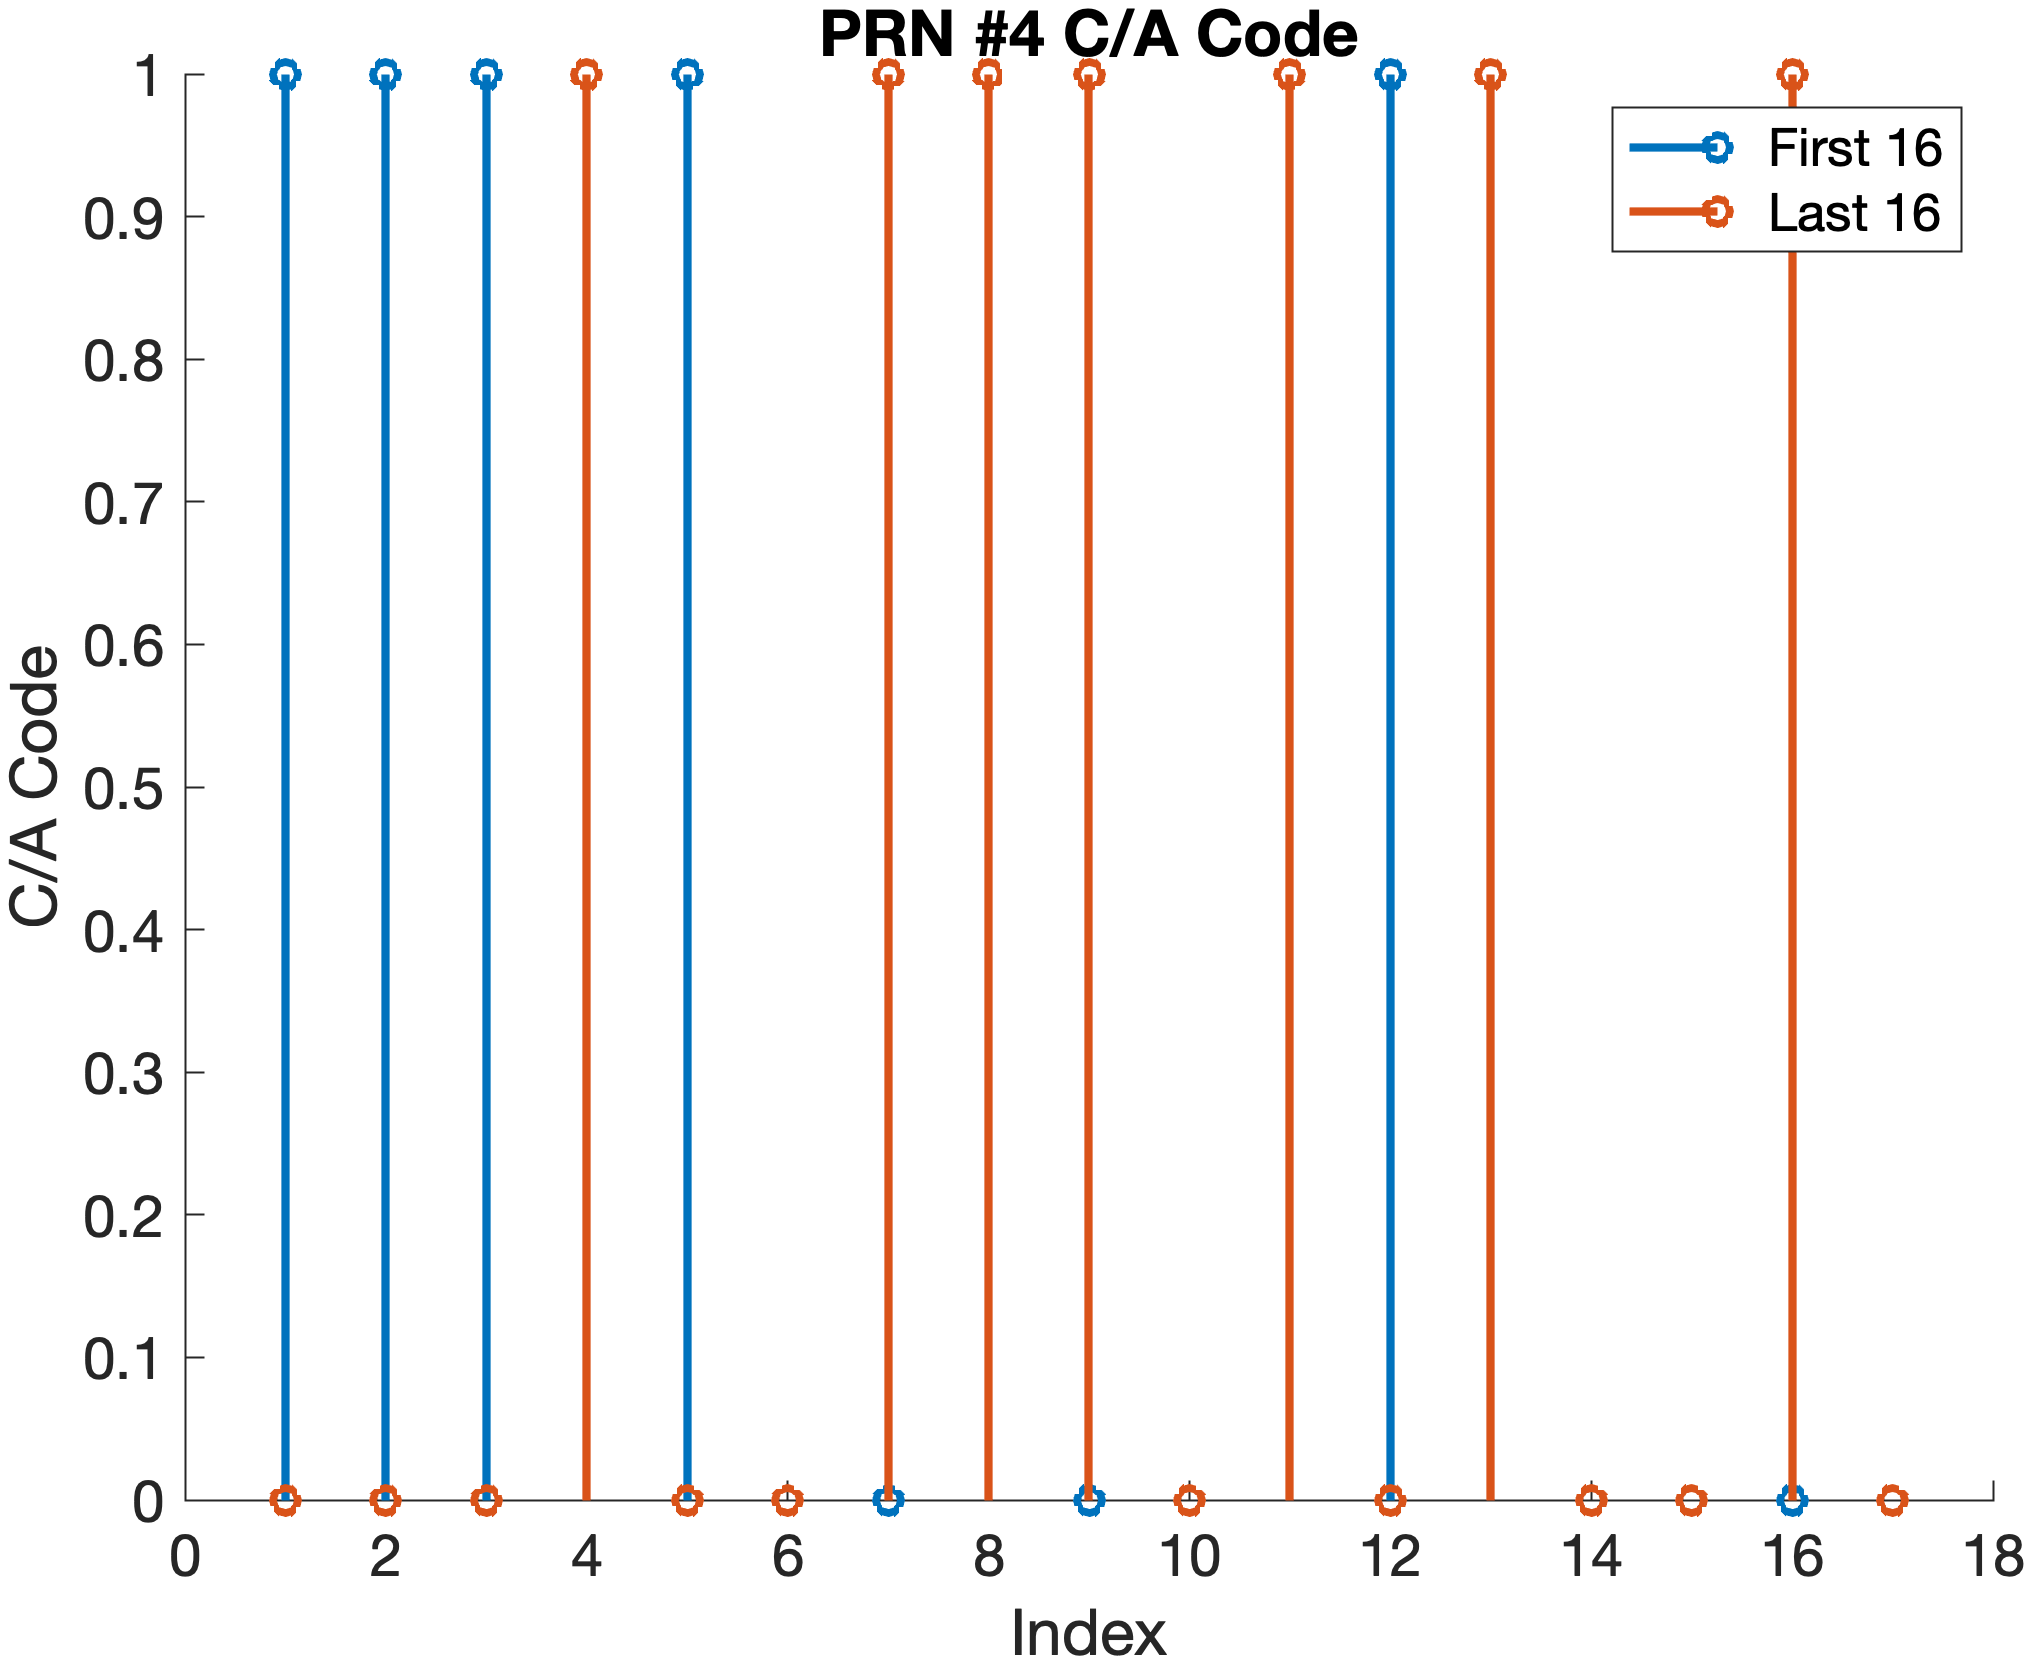
\includegraphics[width=0.75\linewidth]{../figures/p7_prn4_16.png}\label{fig:p7_prn4_16}
    \caption{First 16 bits of C/A Code for PRN 4}
\end{figure}
\begin{figure}[H]
    \centering
    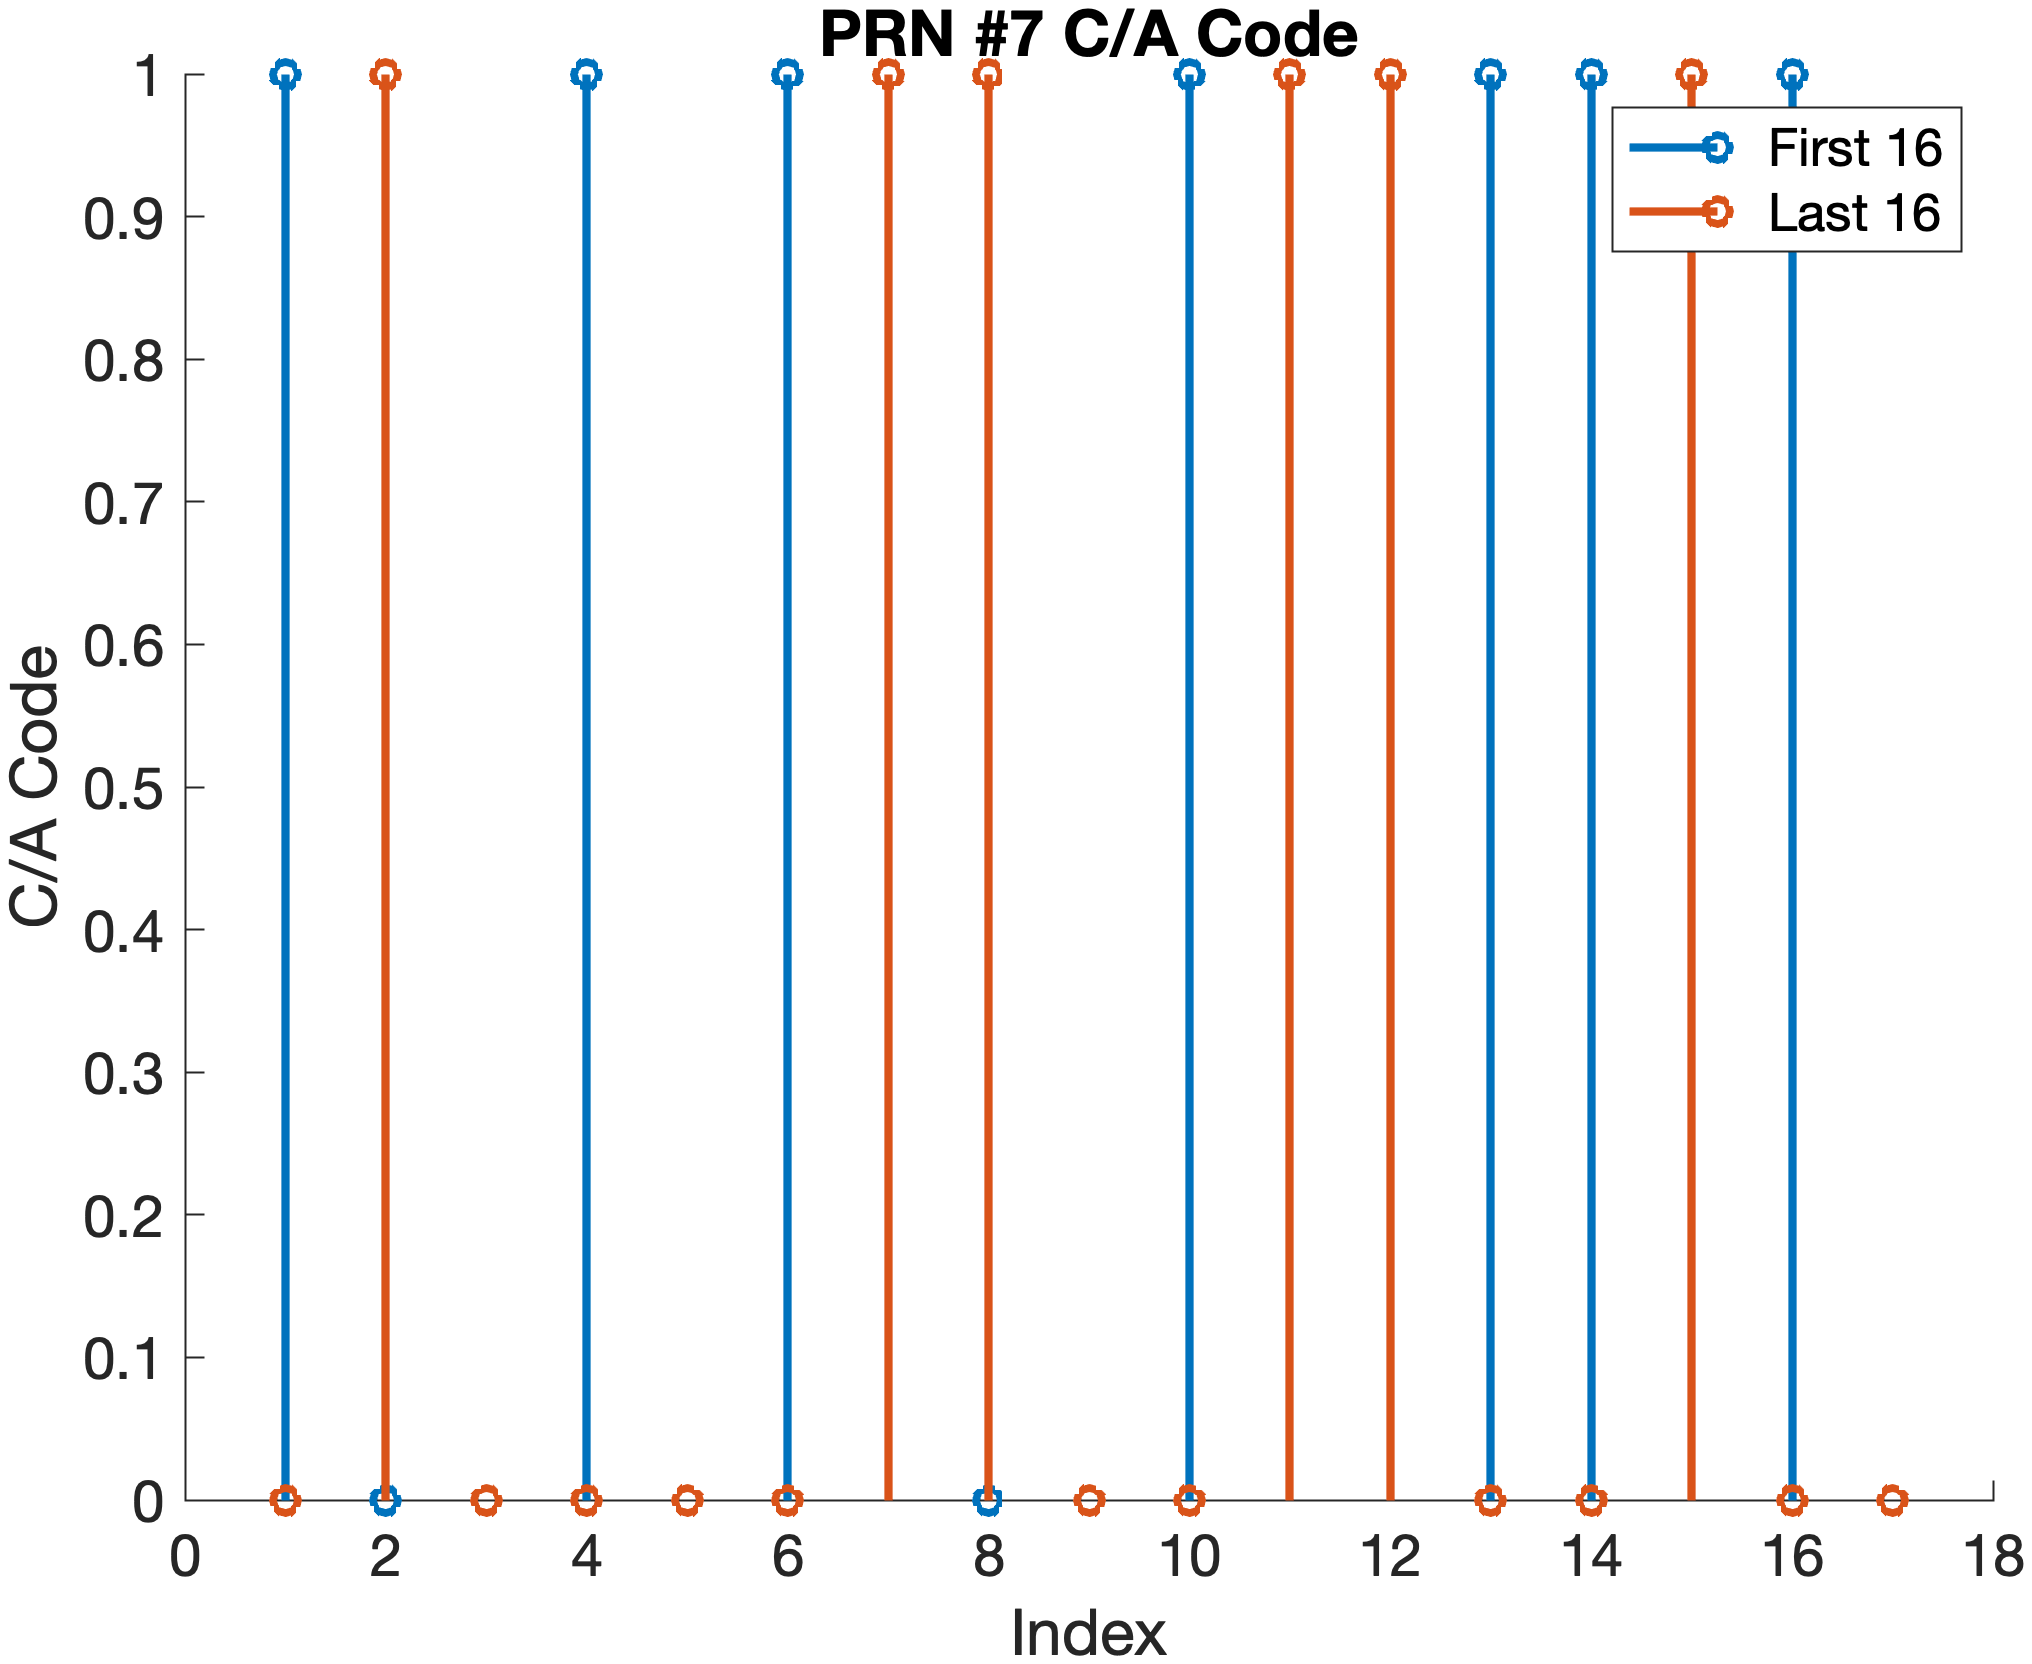
\includegraphics[width=0.75\linewidth]{../figures/p7_prn7_16.png}\label{fig:p7_prn7_16}
    \caption{First 16 bits of C/A Code for PRN 7}
\end{figure}

\section*{Problem VIII}
Using your PRN sequence for PRN 4 and 7, repeat problem \#2 from HW\#1. Compare the
results to the results for your made up sequence.

\subsection*{Solution}
PUT STUFF HERE

\subsection*{Part A}
Plot the histogram on each sequence

\subsection*{Solution}
\begin{figure}[H]
    \centering
    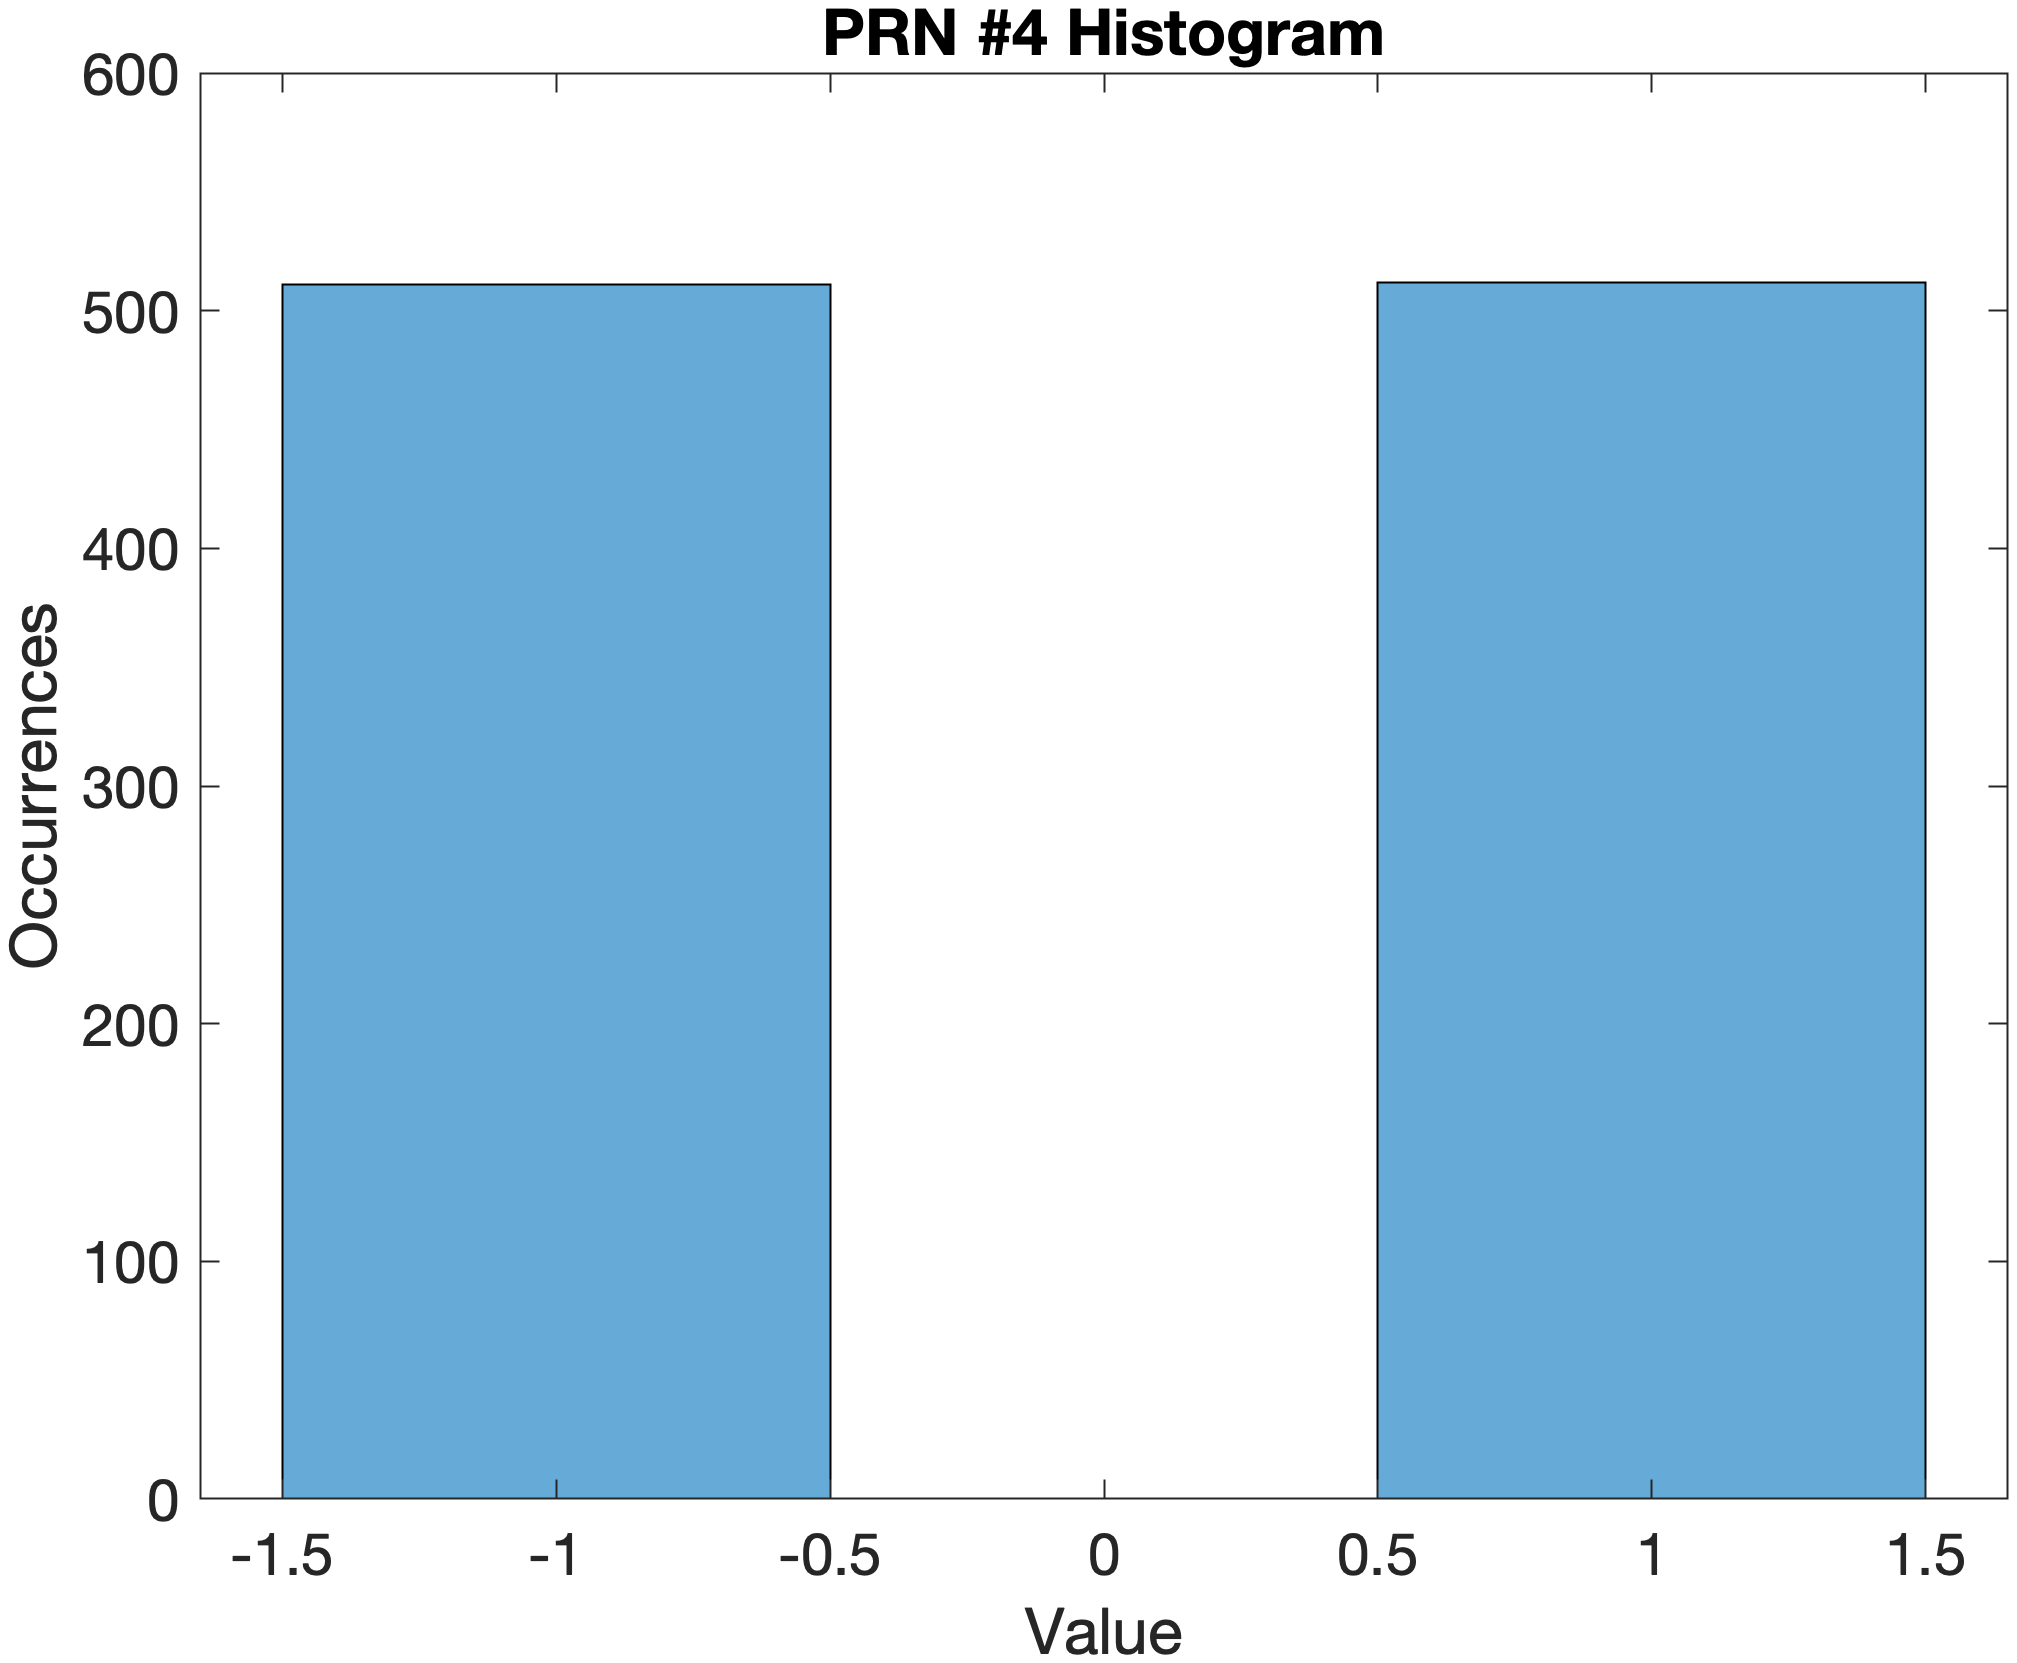
\includegraphics[width=0.75\linewidth]{../figures/p8_prn4_hist.png}\label{fig:p8_prn4_hist}
    \caption{PRN 4 Histogram }
\end{figure}

\begin{figure}[H]
    \centering
    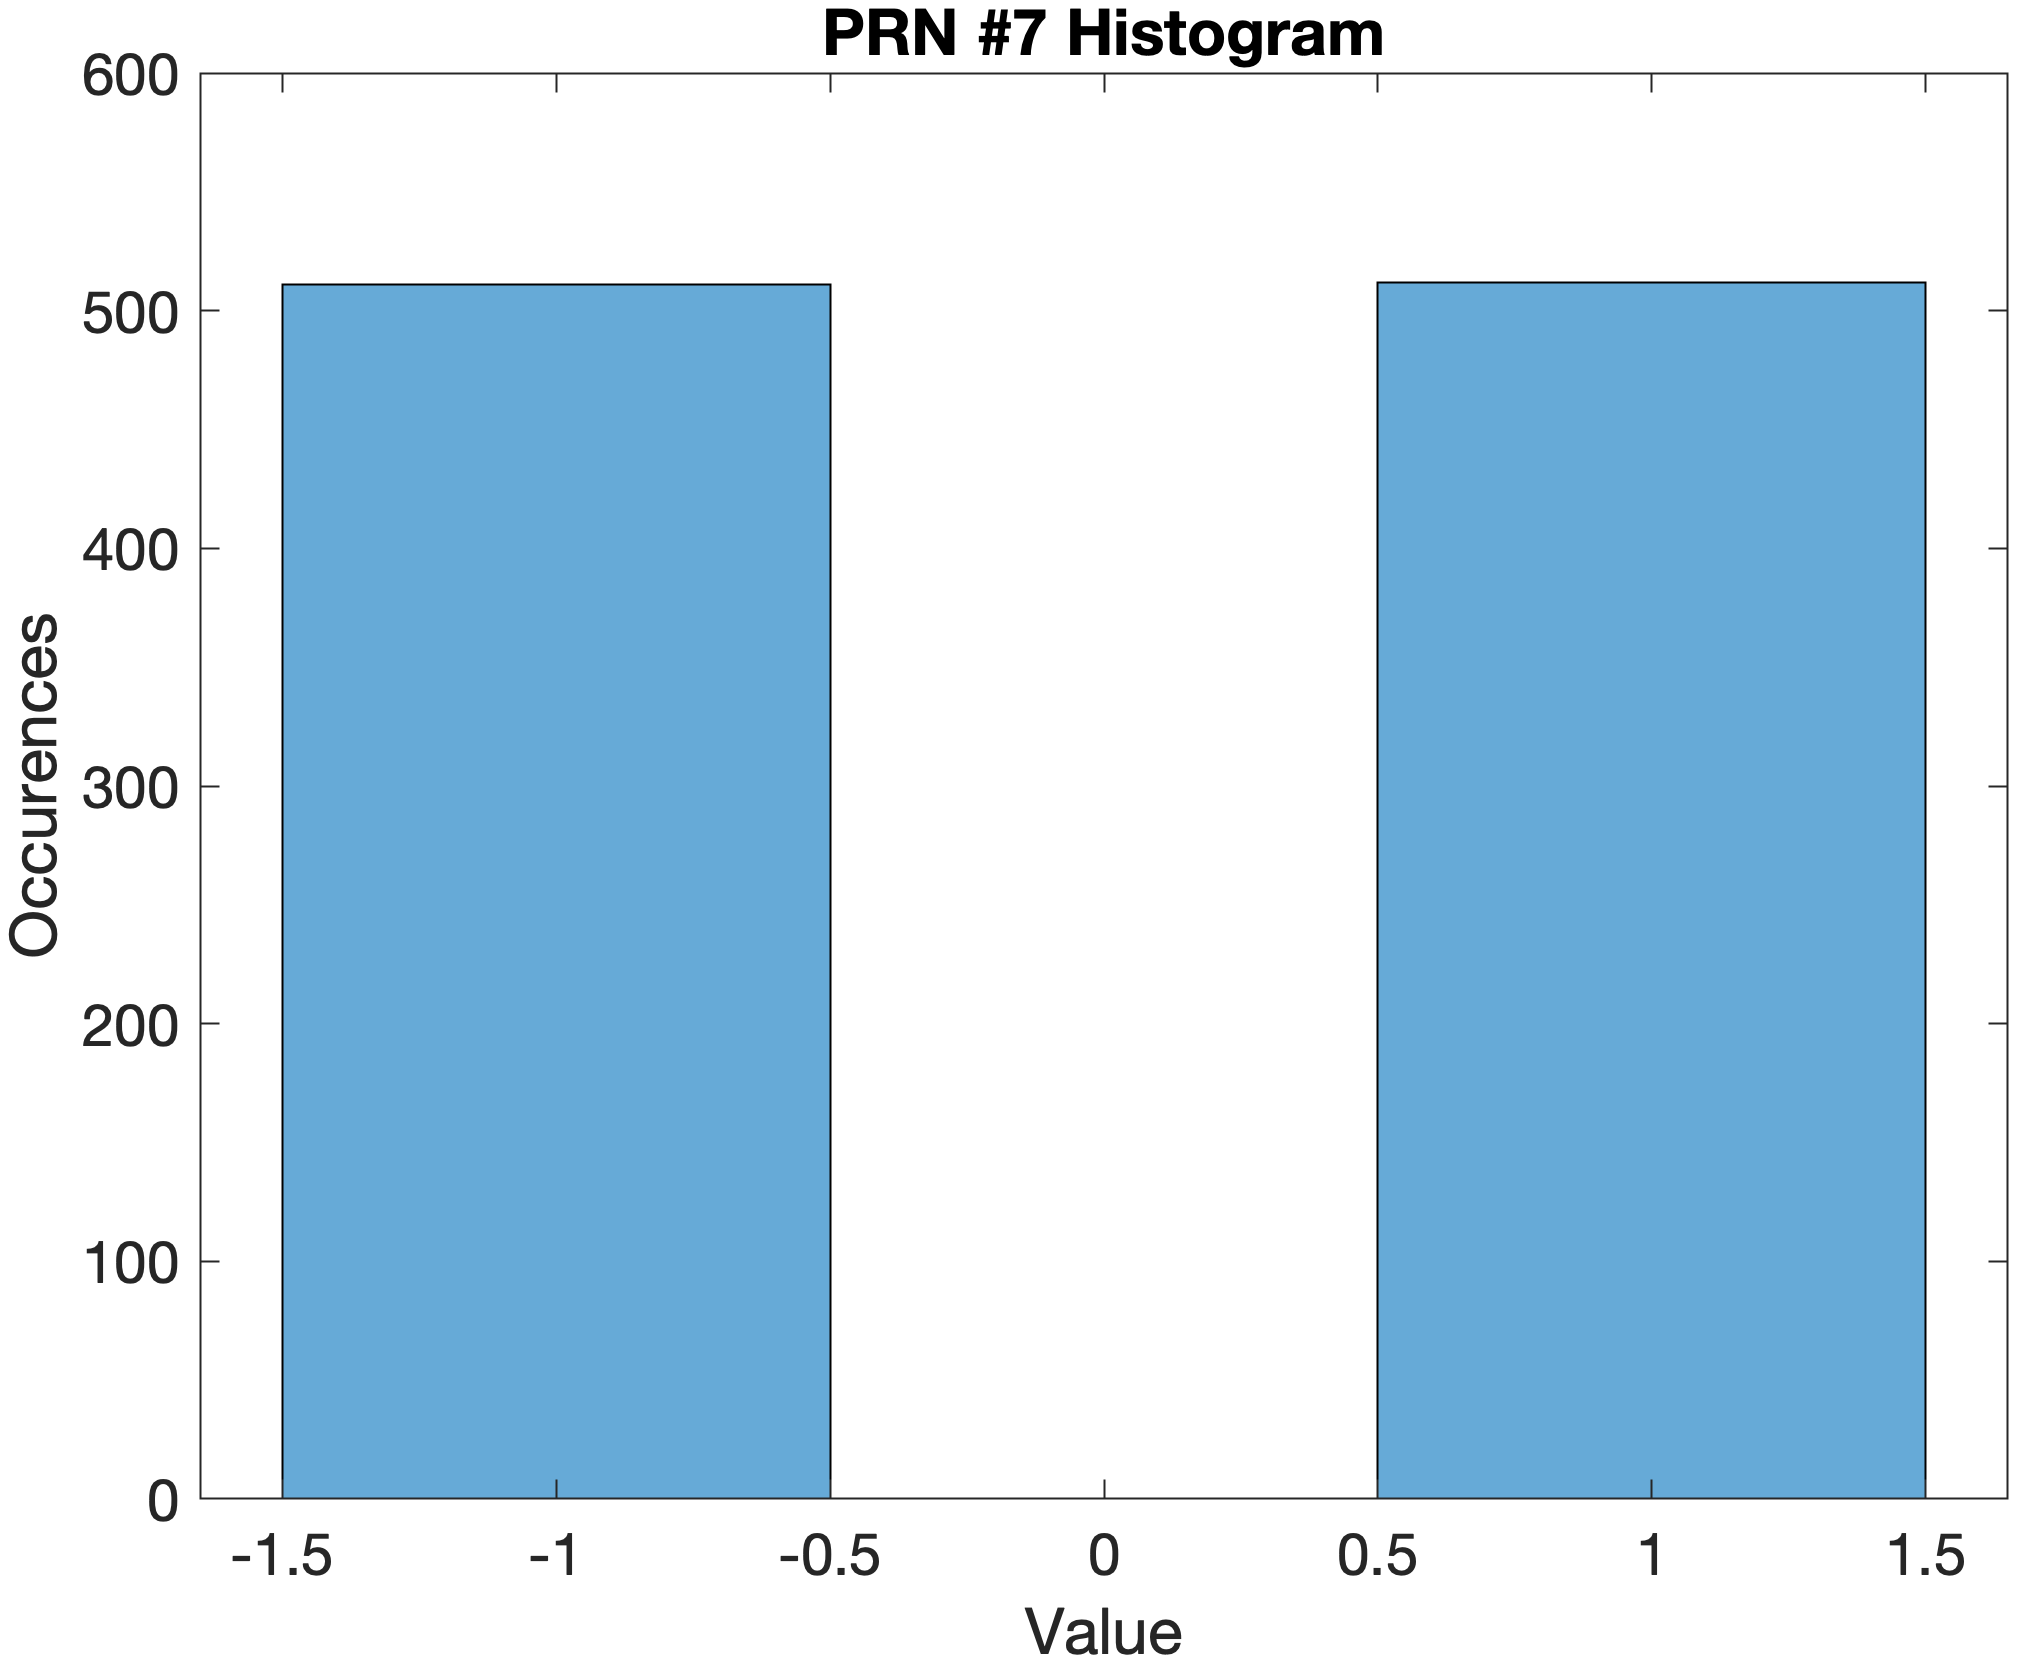
\includegraphics[width=0.75\linewidth]{../figures/p8_prn7_hist.png}\label{fig:p8_prn7_hist}
    \caption{PRN 7 Histogram }
\end{figure}

\subsection*{Part B}
Plot the spectral analysis on each sequence

\subsection*{Solution}
\begin{figure}[H]
    \centering
    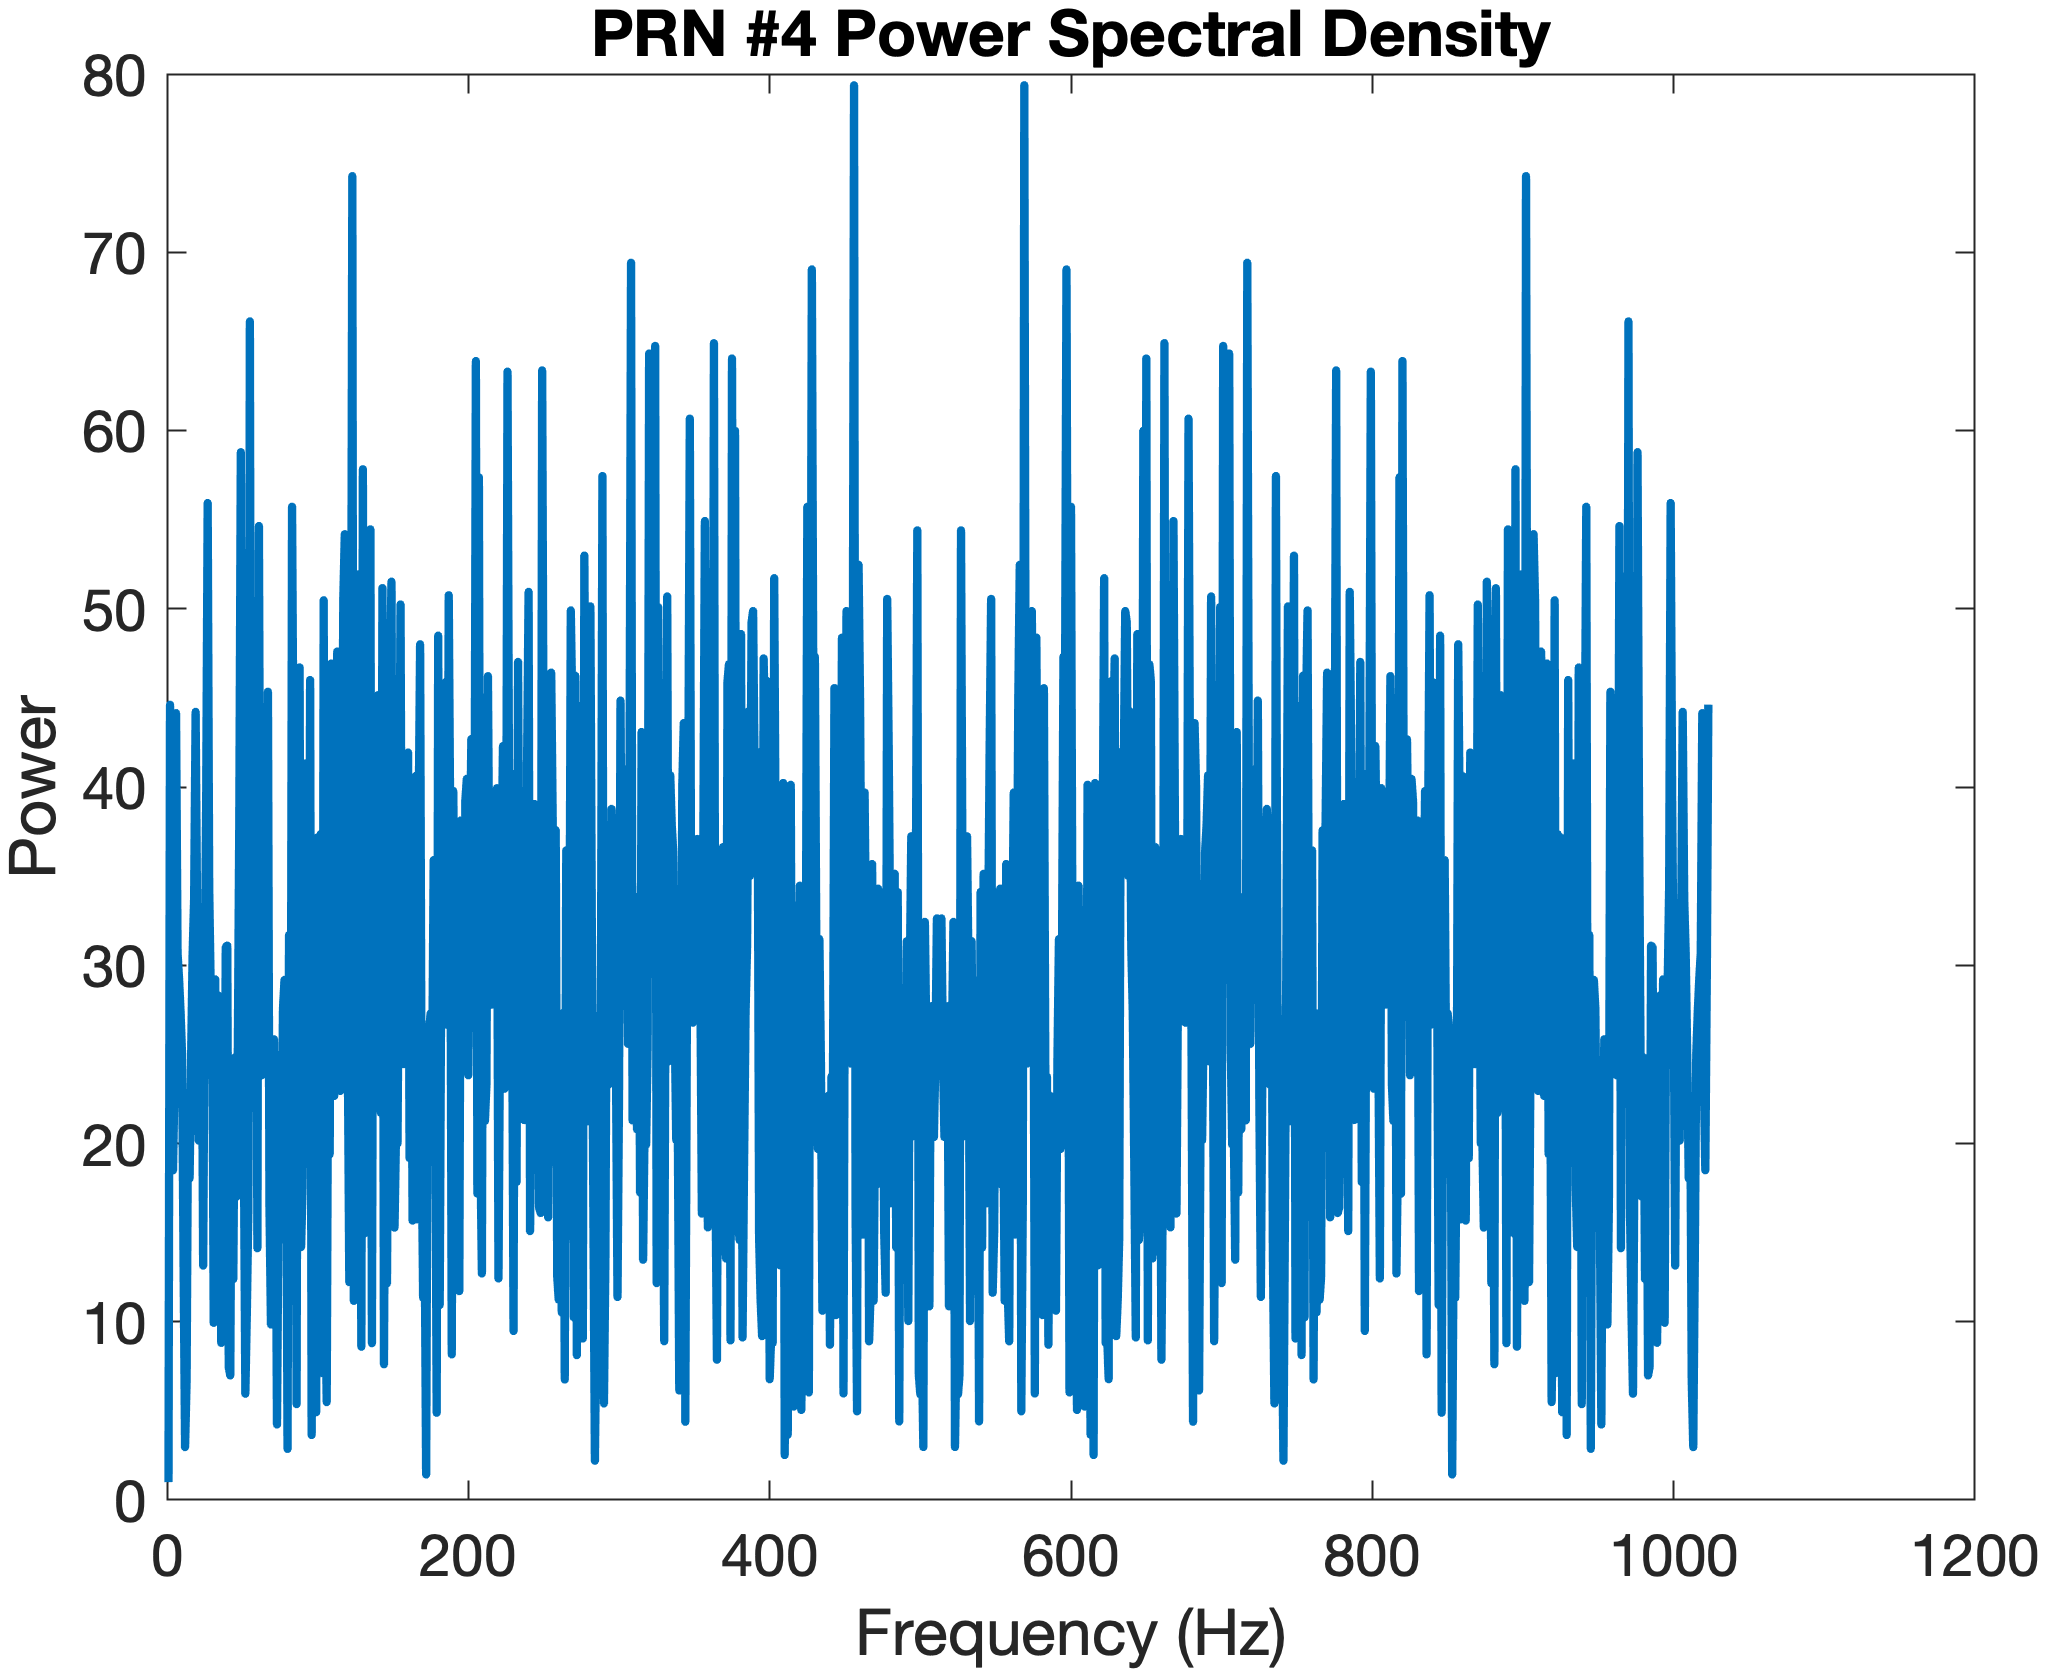
\includegraphics[width=0.75\linewidth]{../figures/p8_prn4_psd.png}\label{p8_prn4_psd}
    \caption{PRN 4 Power Spectral Density}
\end{figure}
\begin{figure}[H]
    \centering
    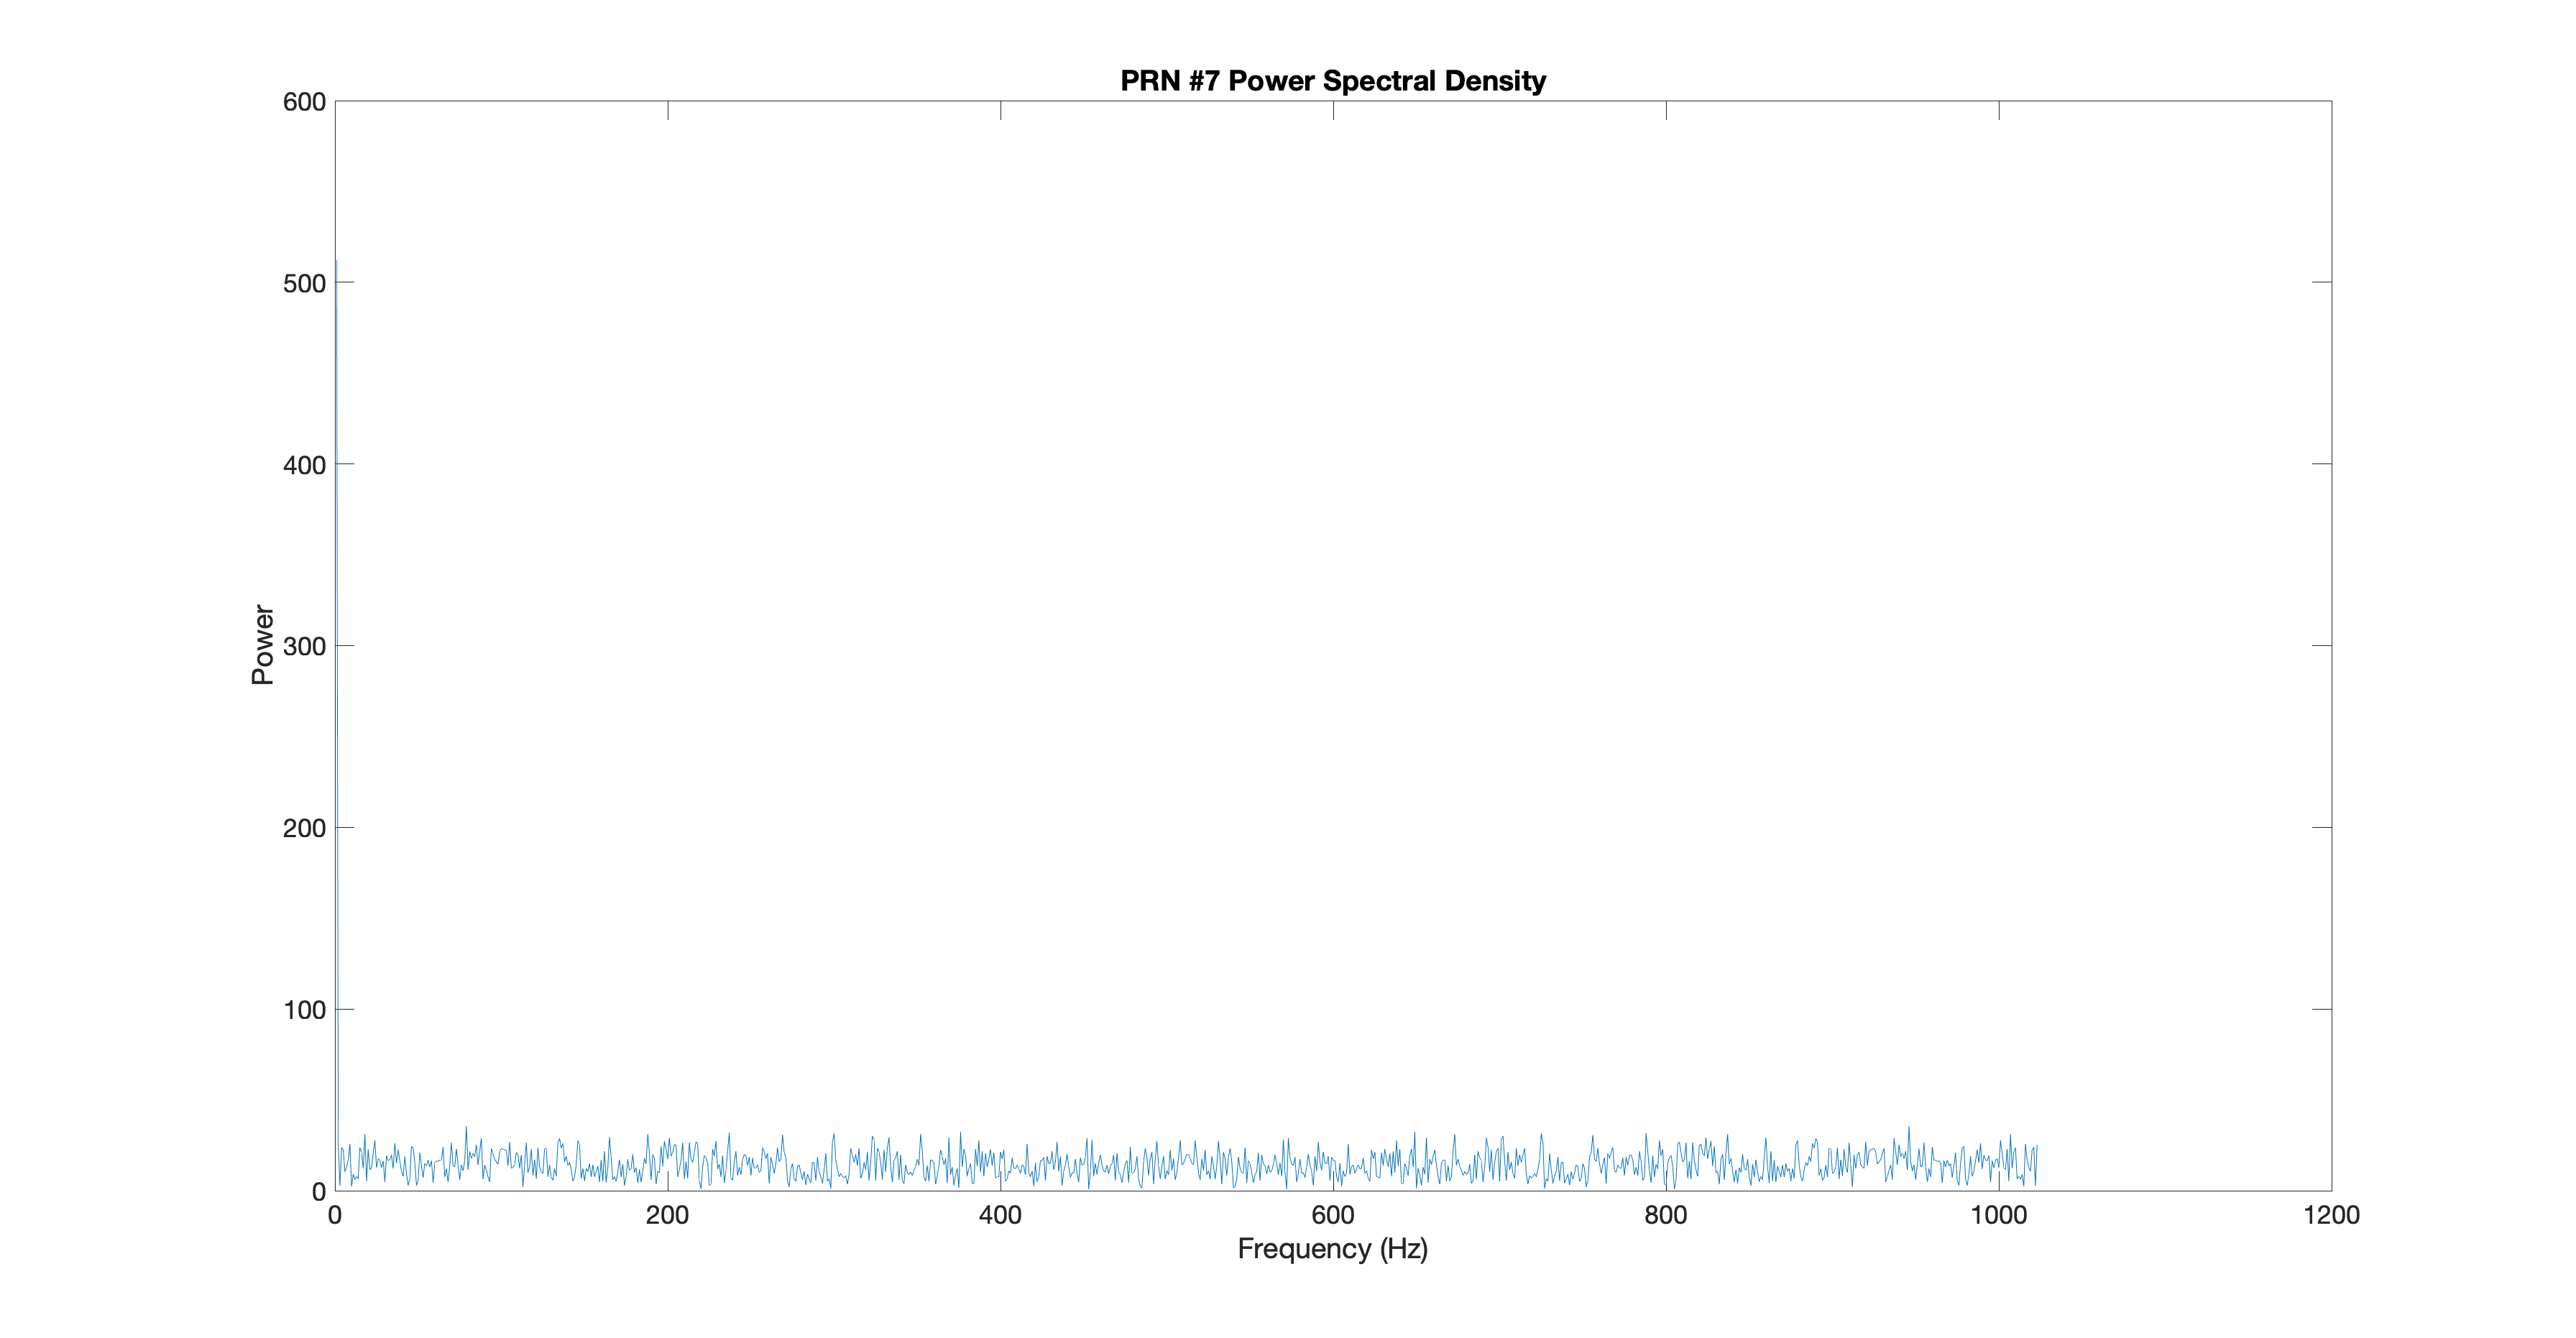
\includegraphics[width=0.75\linewidth]{../figures/p8_prn7_psd.png}\label{p8_prn7_psd}
    \caption{PRN 7 Power Spectral Density}
\end{figure}

\subsection*{Part C}
Plot the auto correlation each sequence with itself (i.e. a sequence delay cross
correlation)

\subsection*{Solution}
\begin{figure}[H]
    \centering
    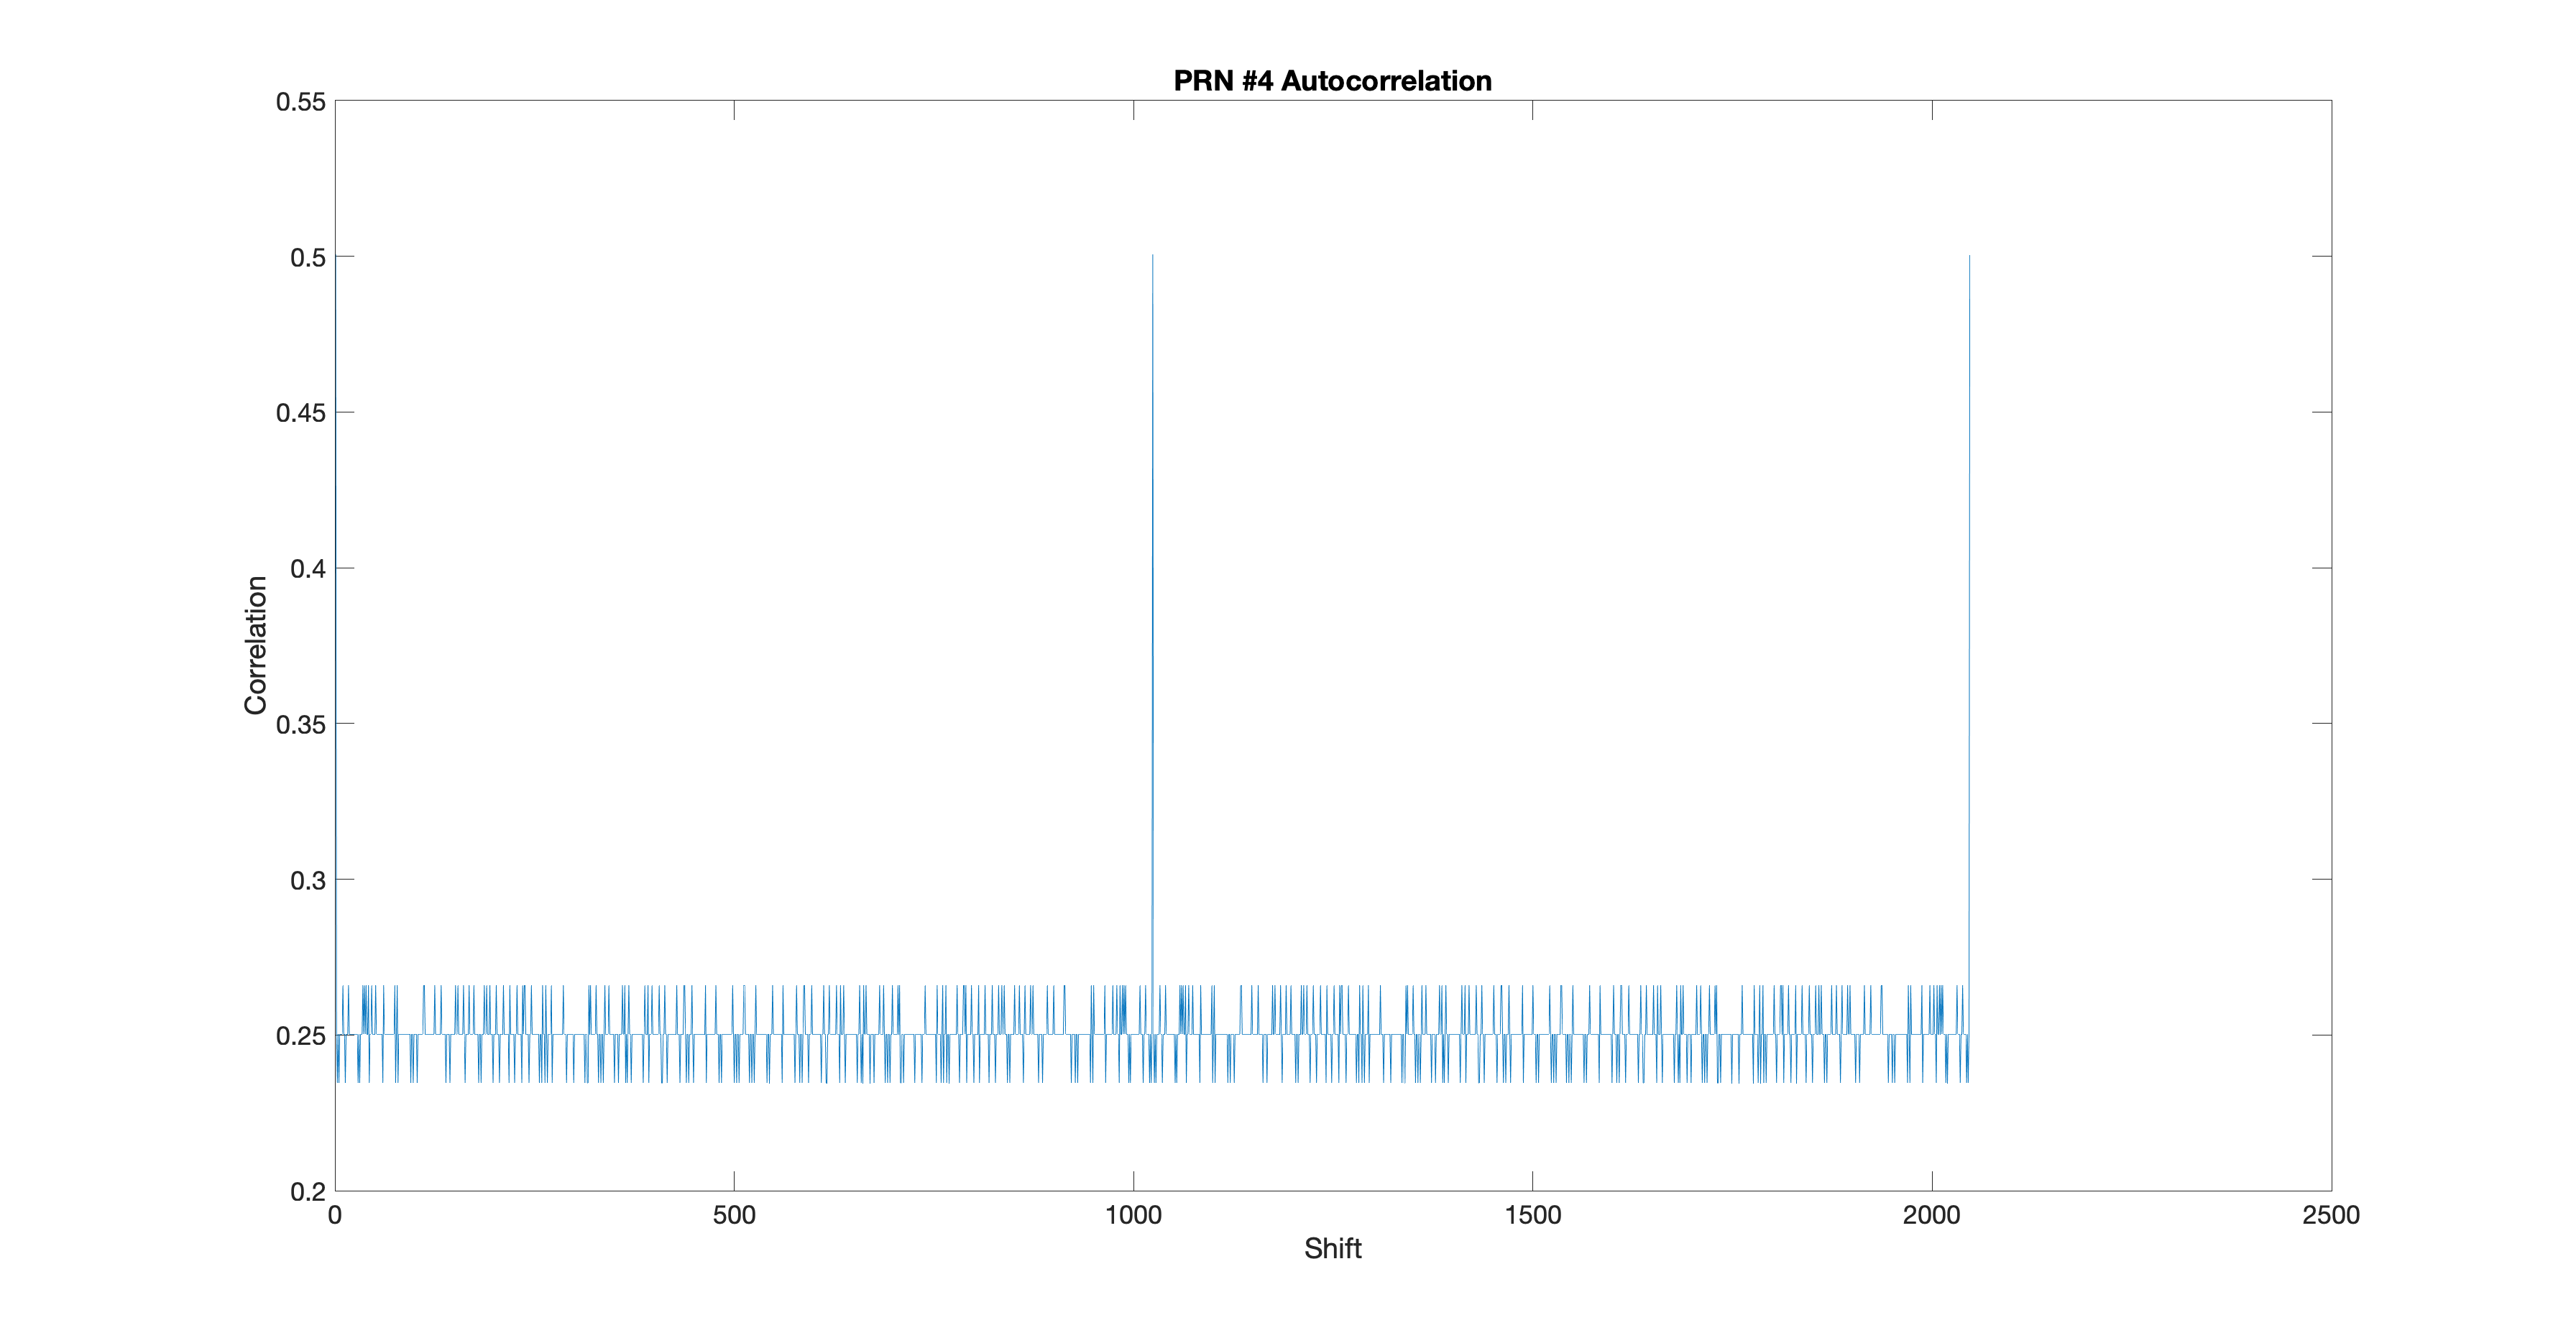
\includegraphics[width=0.75\linewidth]{../figures/p8_prn4_acorr.png}\label{p8_prn4_acorr}
    \caption{PRN 4 Autocorrelation}
\end{figure}
\begin{figure}[H]
    \centering
    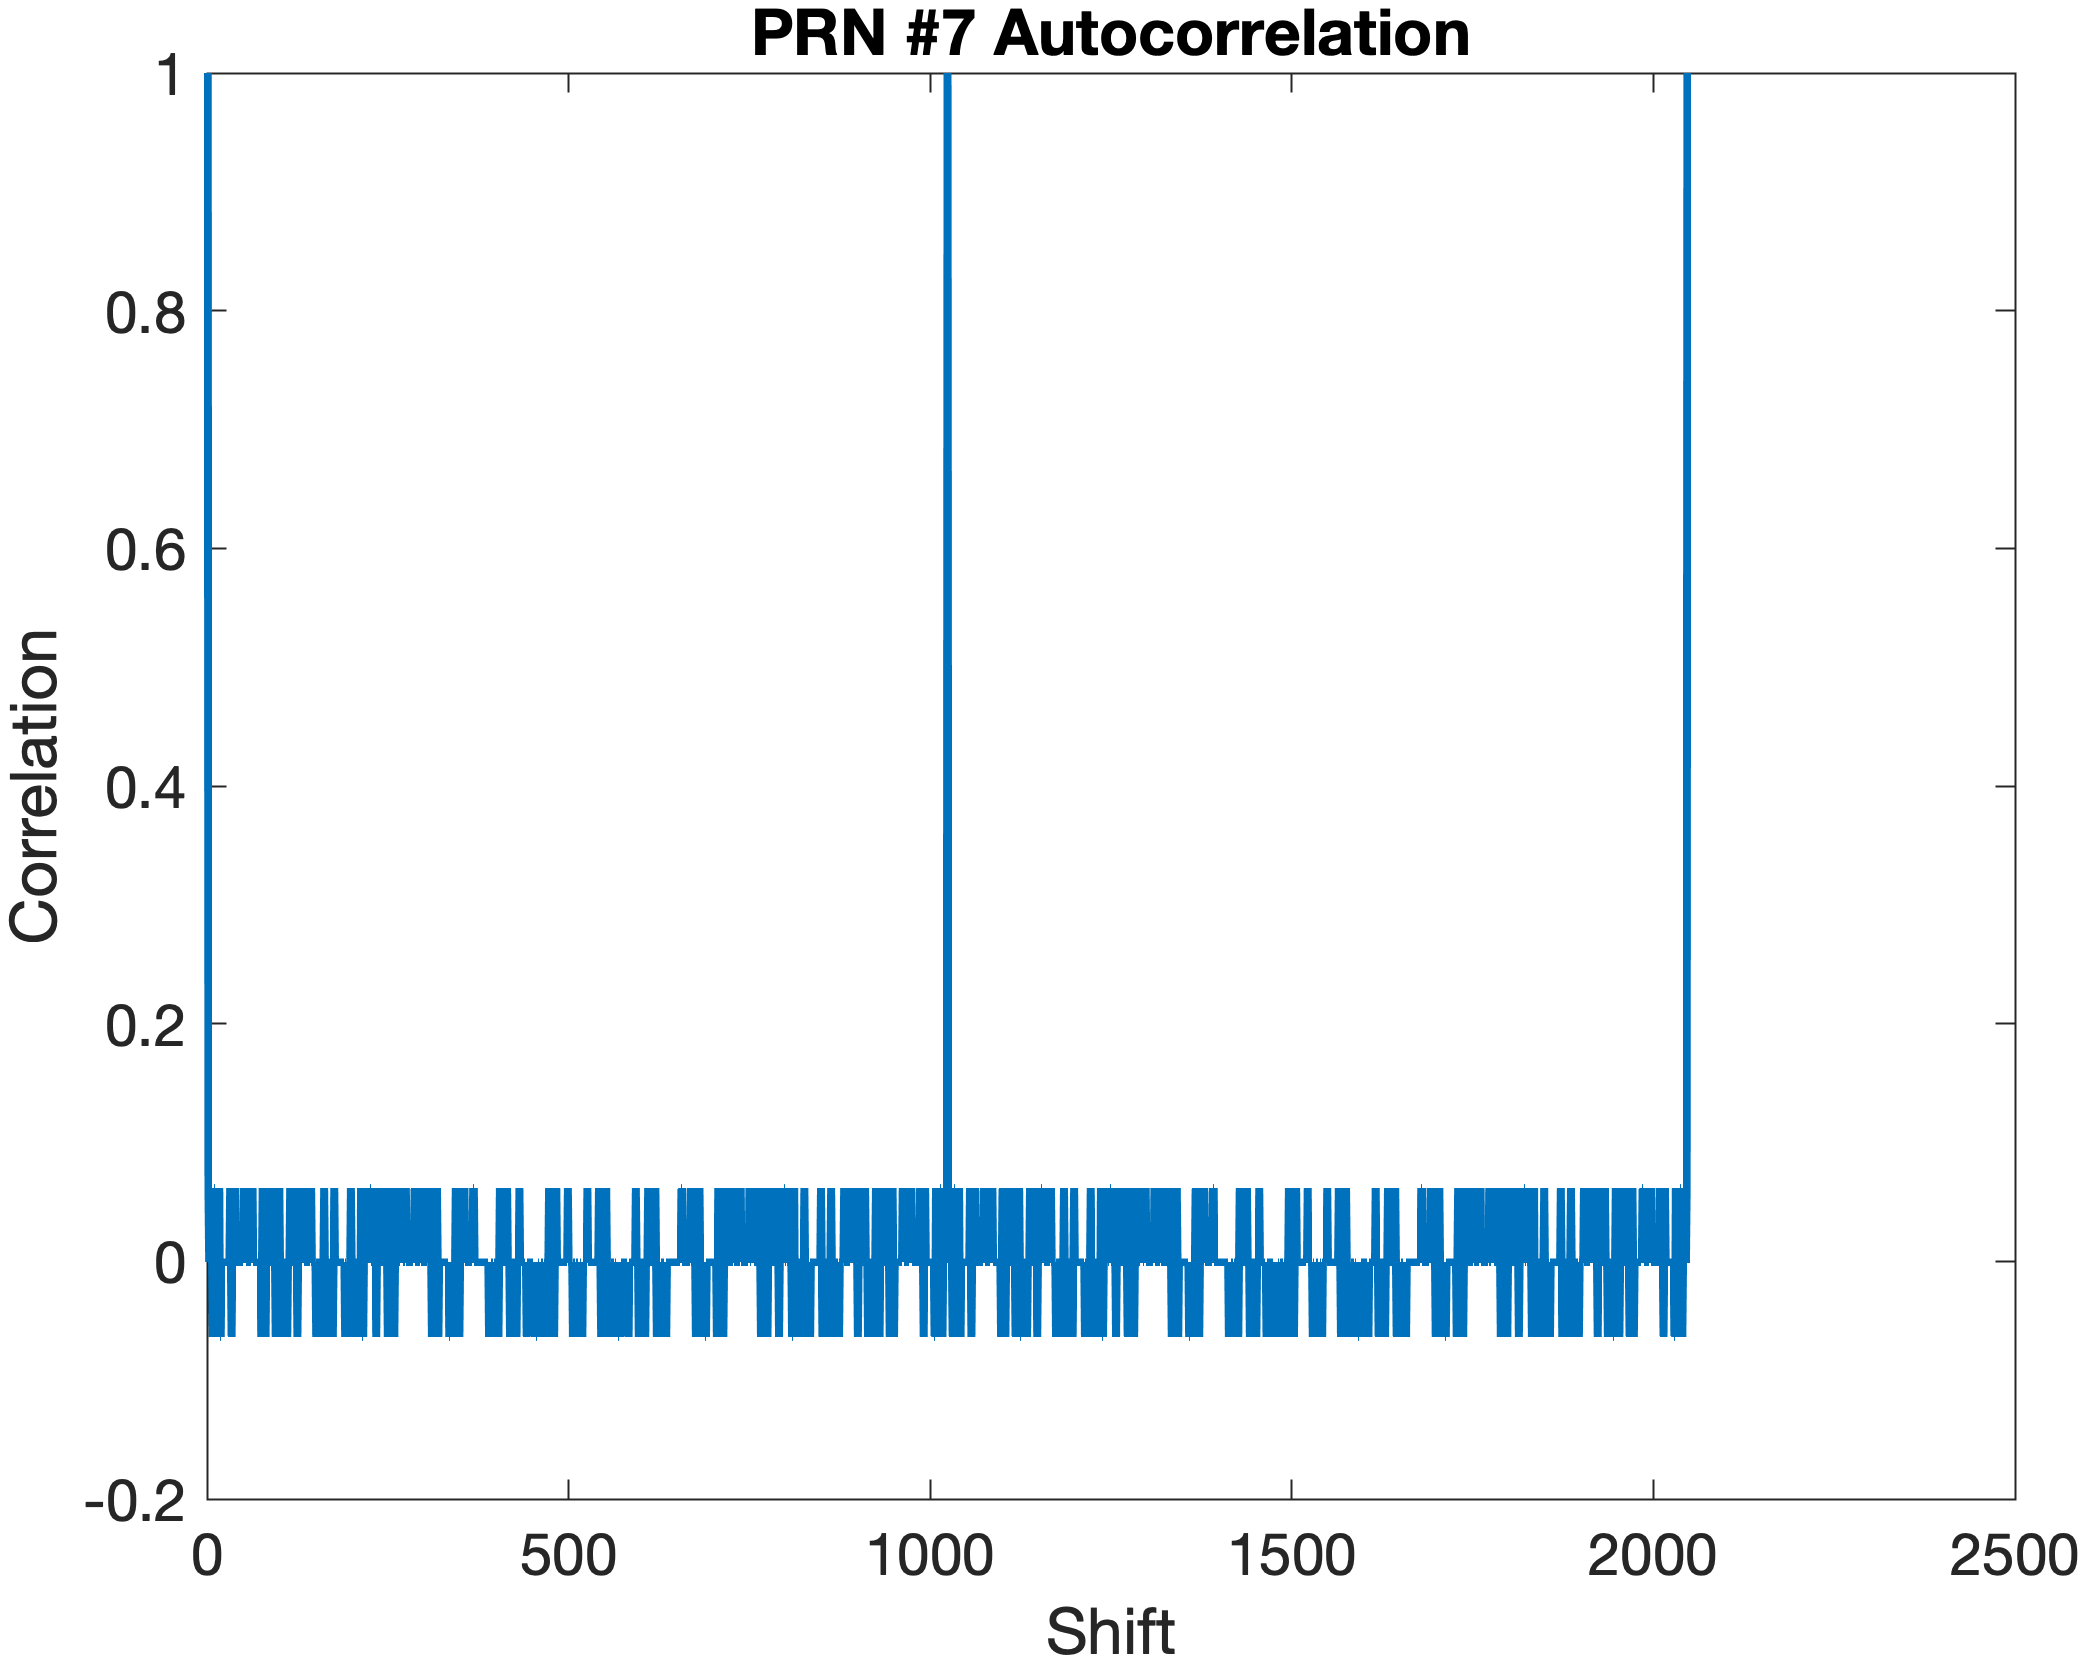
\includegraphics[width=0.75\linewidth]{../figures/p8_prn7_acorr.png}\label{p8_prn7_acorr}
    \caption{PRN 7 Autocorrelation}
\end{figure}

\subsection*{Part D}
Plot the cross auto correlation between the two sequences

\subsection*{Solution}
\begin{figure}[H]
    \centering
    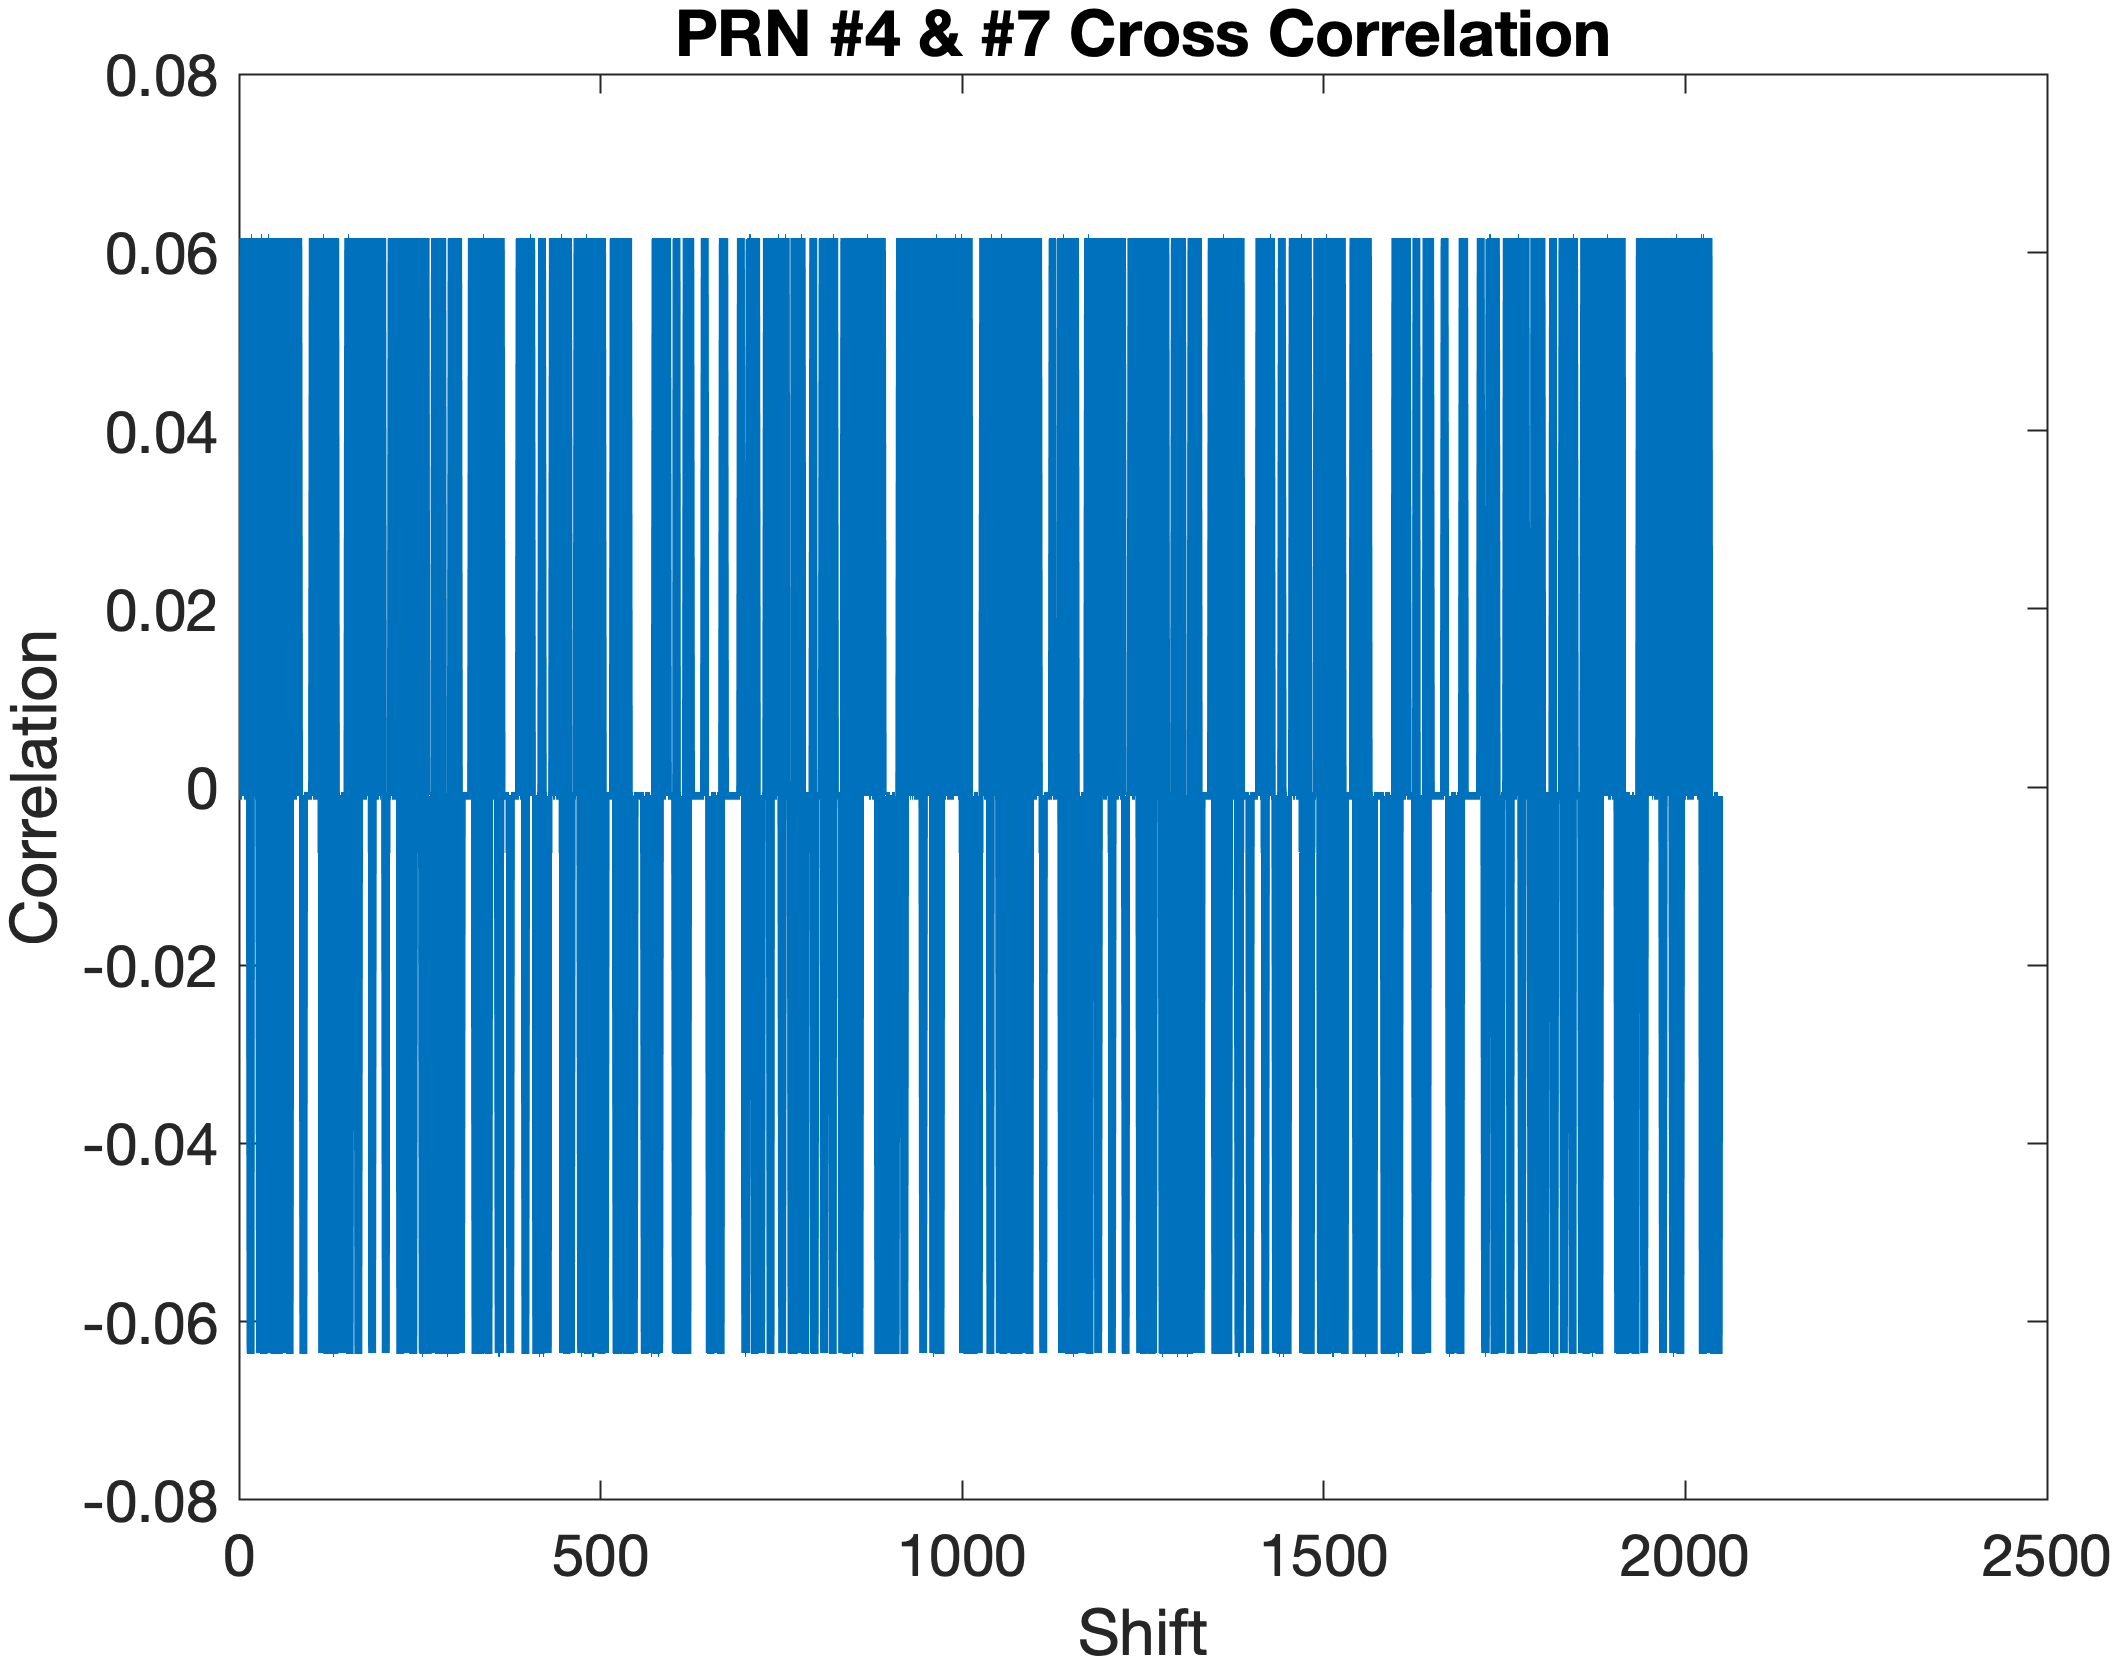
\includegraphics[width=0.75\linewidth]{../figures/p8_prn47_xcorr.png}\label{p8_prn47_xcorr}
    \caption{PRN 4 \& 7 Cross Correlation}
\end{figure}

\section*{Problem IX}
Take your C/A code from problem above (i.e. PRN \#4 and \#7) and multiply it times the L1
Carrier (your C/A code must be in the form -1 and +1). Perform a spectral analysis
(magnitude) on the resultant signal. You will need to make sure to “hold” your C/A code bits
for the correct length of time (I suggest using a sample rate 10x the L1 carrier frequency –
meaning each chip of the C/A code will be used for 10 samples of the sine wave).

\subsection*{Solution}
\begin{figure}[H]
    \centering
    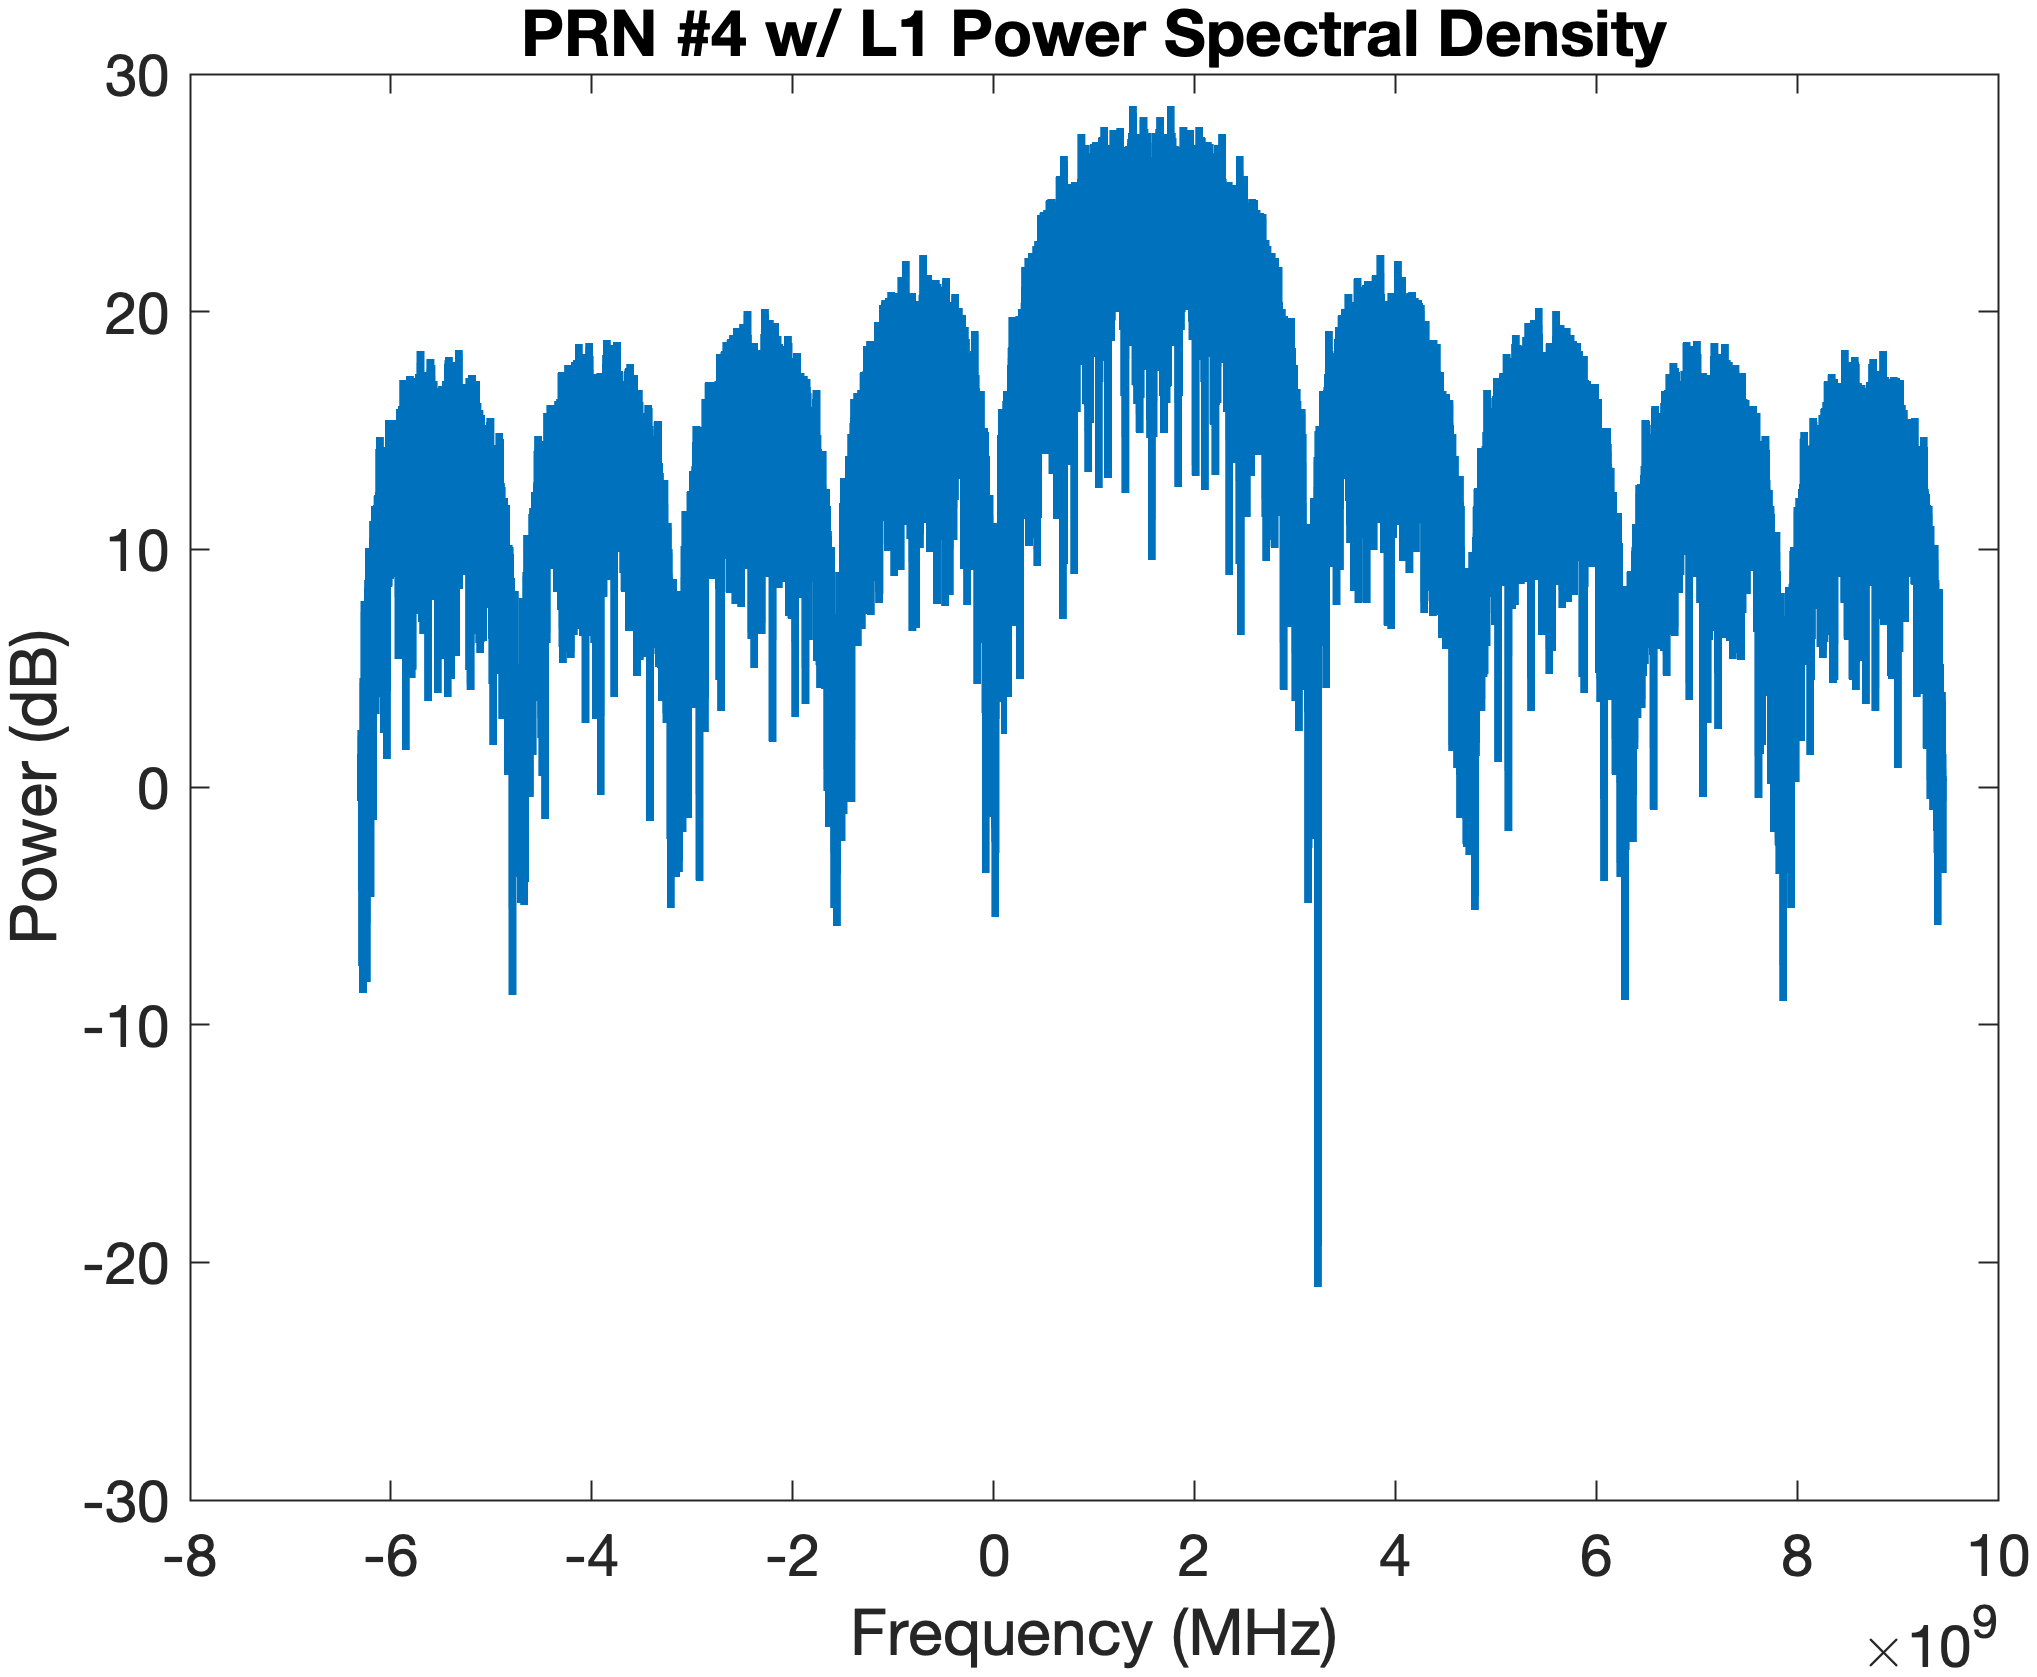
\includegraphics[width=0.75\linewidth]{../figures/p9_prn4_psd.png}\label{p9_prn4_psd}
    \caption{C/A Code for PRN 4 + L1 Carrier PSD}
\end{figure}

\begin{figure}[H]
    \centering
    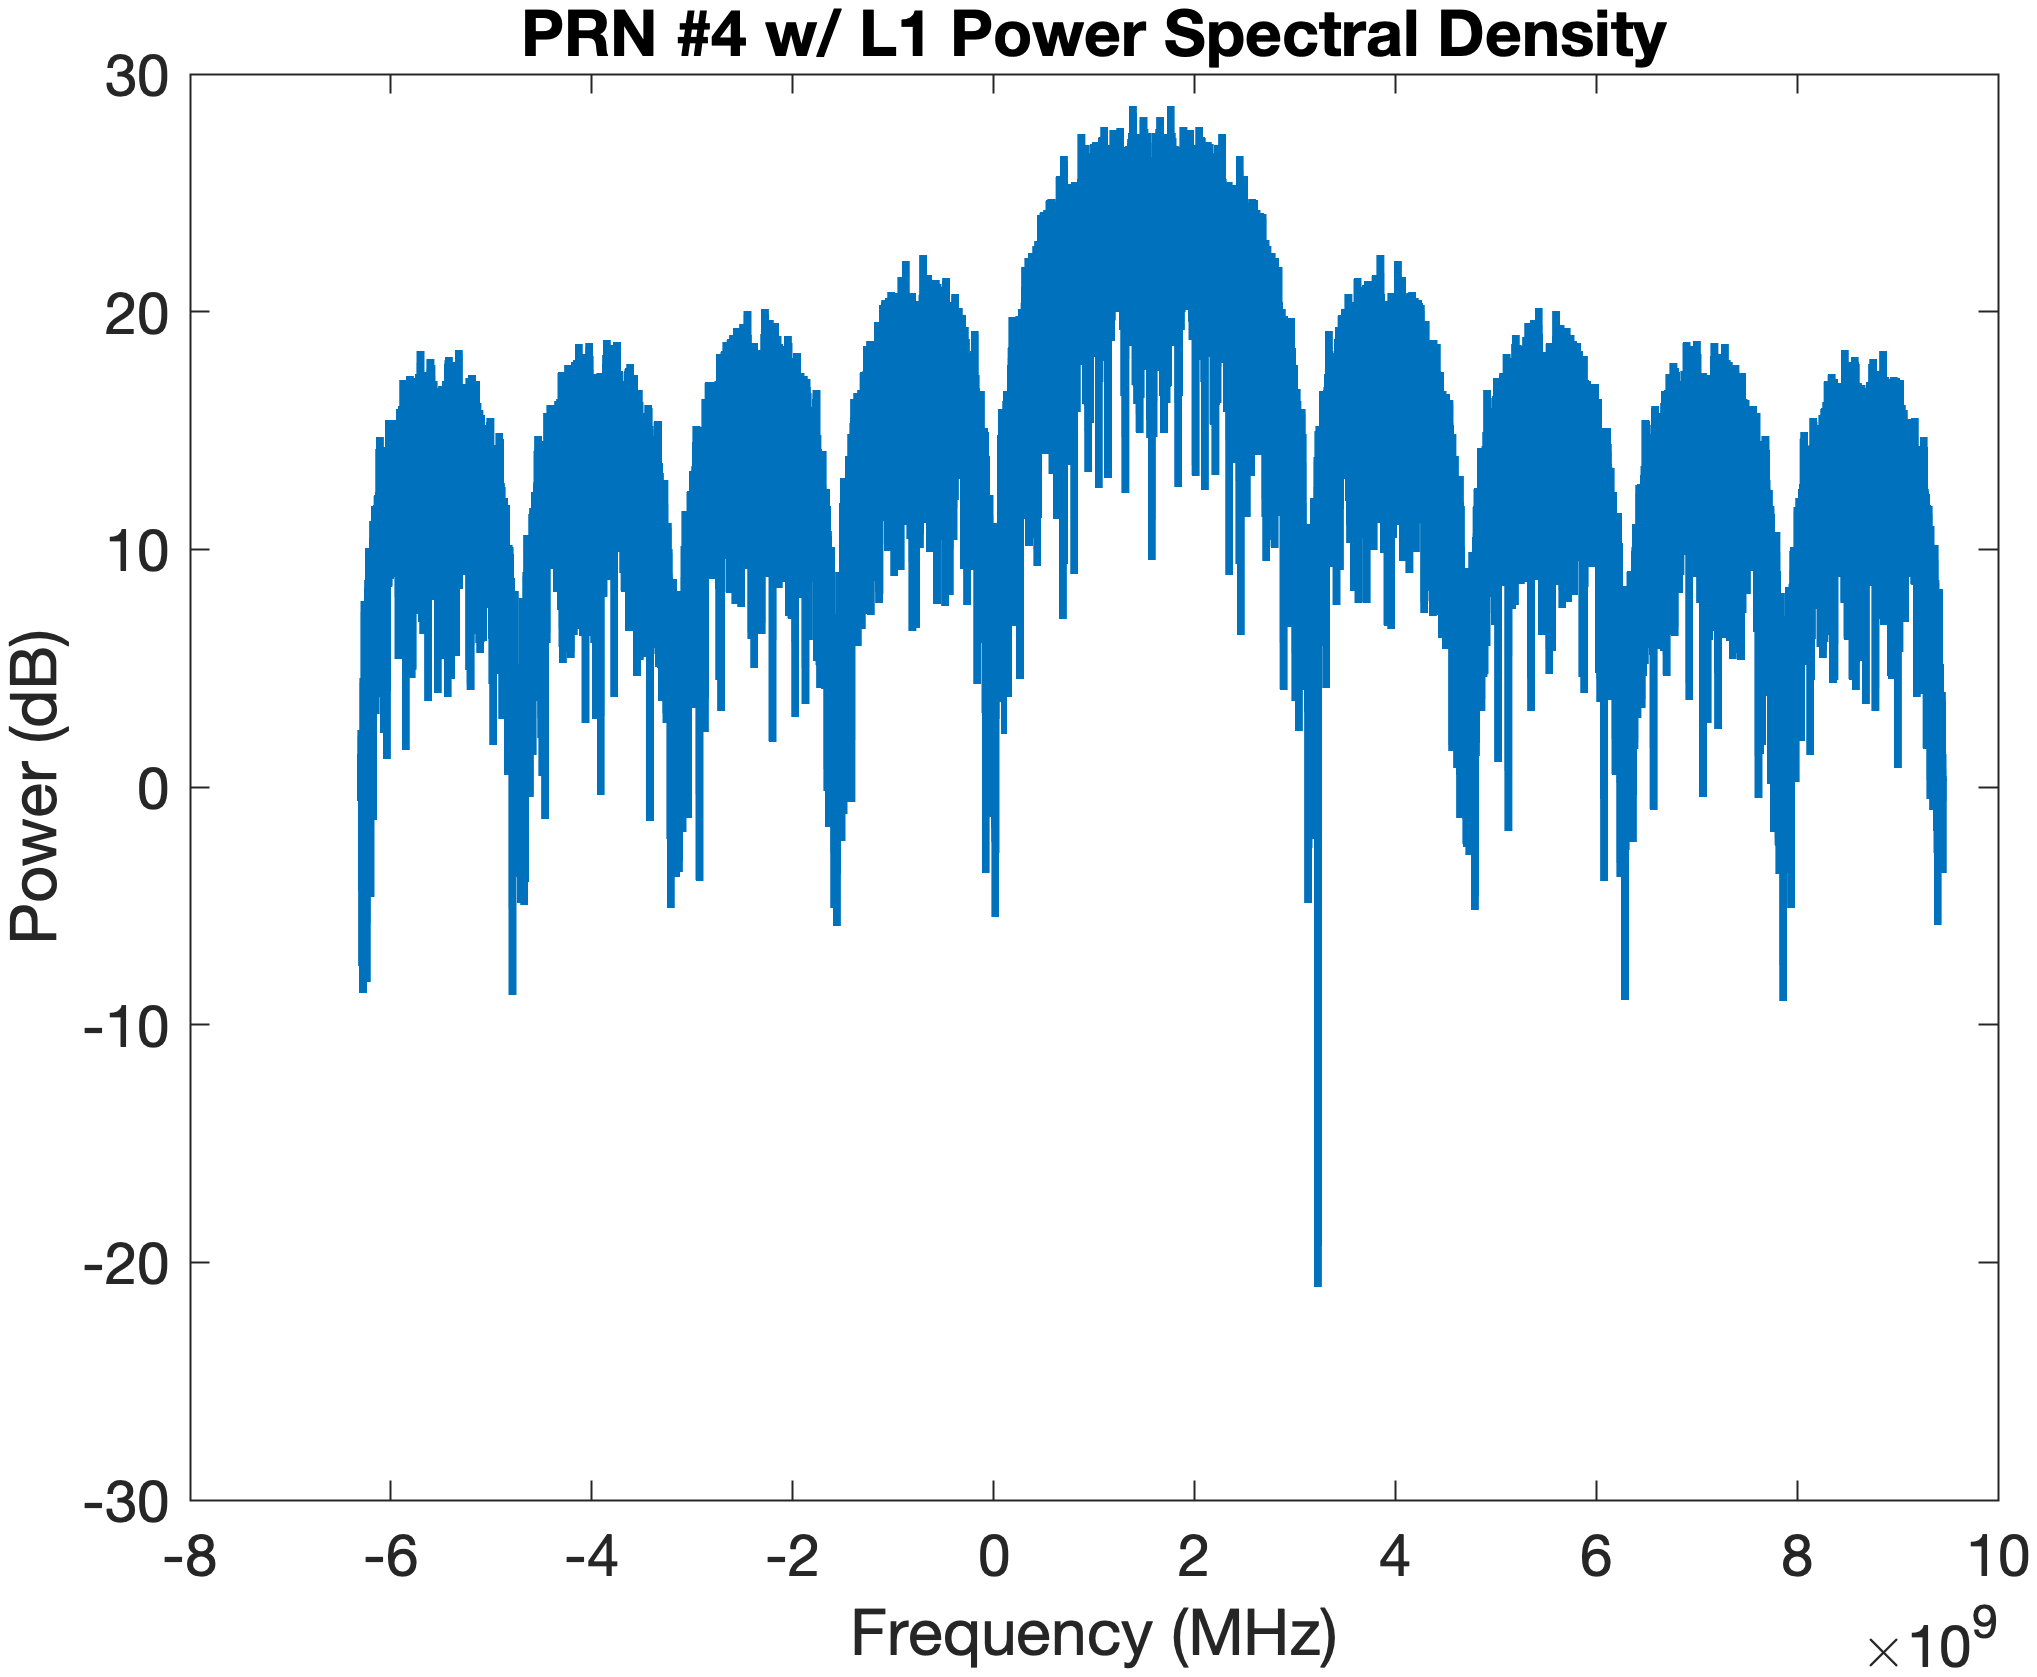
\includegraphics[width=0.75\linewidth]{../figures/p9_prn4_psd.png}\label{p9_prn4_psd}
    \caption{C/A Code for PRN 4 + L1 Carrier PSD}
\end{figure}

\end{document}
